% Template for a Computer Science Tripos Part II project dissertation
\documentclass[12pt,a4paper,twoside,openright]{report}
\usepackage[pdfborder={0 0 0}]{hyperref}    % turns references into hyperlinks
\usepackage[margin=25mm]{geometry}  % adjusts page layout
% allows inclusion of PDF, PNG and JPG images
\usepackage{graphicx}
\graphicspath{ {figs/}}

% For plots
\newlength\figureheight
\newlength\figurewidth
\usepackage{pgfplots}

\usepackage{amsmath}
\usepackage{amssymb}
\usepackage{bbm} %Used for the indicator function
\newcommand{\argmax}[1]{\underset{#1}{\operatorname{arg}\,\operatorname{max}}\;} %specifies the argmax command

\usepackage{algorithm}
\usepackage{algpseudocode}

\usepackage{siunitx} %For better alignement of numbers in tables. 

\usepackage{verbatim}
\usepackage{docmute}   % only needed to allow inclusion of proposal.tex

\usepackage{multirow}
\usepackage{hhline} % Draw partial double lines in tables

\usepackage{listings} % Package to display code and customize highlighting
\usepackage{color}
 
\definecolor{codegreen}{rgb}{0,0.6,0}
\definecolor{codegray}{rgb}{0.5,0.5,0.5}
\definecolor{codepurple}{rgb}{0.58,0,0.82}
\definecolor{backcolour}{rgb}{0.95,0.95,0.92}
 
\lstdefinestyle{mystyle}{
    backgroundcolor=\color{backcolour},   
    commentstyle=\color{codegreen},
    keywordstyle=\color{magenta},
    numberstyle=\tiny\color{codegray},
    stringstyle=\color{codepurple},
    basicstyle=\footnotesize,
    breakatwhitespace=false,         
    breaklines=true,                 
    captionpos=b,                    
    keepspaces=true,                 
    numbers=left,                    
    numbersep=5pt,                  
    showspaces=false,                
    showstringspaces=false,
    showtabs=false,                  
    tabsize=2
}
\lstset{style=mystyle} % Set code listings style

\raggedbottom                           % try to avoid widows and orphans
\sloppy
\clubpenalty1000%
\widowpenalty1000%

\renewcommand{\baselinestretch}{1.1}    % adjust line spacing to make
                                        % more readable

\begin{document}

\bibliographystyle{plain}


%%%%%%%%%%%%%%%%%%%%%%%%%%%%%%%%%%%%%%%%%%%%%%%%%%%%%%%%%%%%%%%%%%%%%%%%
% Title


\pagestyle{empty}

\rightline{\LARGE \textbf{Sebastian Borgeaud dit Avocat}}

\vspace*{60mm}
\begin{center}
\Huge
\textbf{Brain tumour segmentation using Convolutional Neural Networks} \\[5mm]
Computer Science Tripos -- Part II \\[5mm]
Fitzwilliam College \\[5mm]
\today  % today's date
\end{center}

%%%%%%%%%%%%%%%%%%%%%%%%%%%%%%%%%%%%%%%%%%%%%%%%%%%%%%%%%%%%%%%%%%%%%%%%%%%%%%
% Proforma, table of contents and list of figures

\pagestyle{plain}

\chapter*{Proforma}

{\large
\begin{tabular}{lp{12cm}}
Name:               & \bf Sebastian Borgeaud dit Avocat                       \\
College:            & \bf Fitzwilliam College                     \\
Project Title:      & \bf Brain tumour segmentation using Convolutional Neural Networks\\
Examination:        & \bf Computer Science Tripos -- Part II, June 2017  \\
Word Count:         & \bf INSERT  \\
Project Originator: & Duo Wang                    \\
Supervisor:         & Dr. Mateja Jamnik \& Duo Wang                    \\ 
\end{tabular}
}
\footnotetext[1]{This word count was computed
by \texttt{detex diss.tex | tr -cd '0-9A-Za-z $\tt\backslash$n' | wc -w}
}
\stepcounter{footnote}
\section*{Original aims of the project}
The main success criteria for this project was to implement an algorithm based on a convolutional neural network that performs brain tumour segmentation. The second aim was to achieve similar results to those obtained by Pereira et al.\ \cite{pereira}, achieving 90\% of the accuracies obtained in the paper, the current state-of-the-art. This means achieving the Dice scores (0.79, 0.73, 0.67) for the regions `complete' (including classes 2–-4), ‘core’ (classes 3–-4) and ‘enhancing’ (class 4) in the BraTS2013 challenge \cite{brats-proceedings}.

\section*{Completed work}
The first goal has been achieved, replicating the proposed method to obtain a model that learns how to perform brain tumour segmentation. The dice scores obtained are (0.8149, 0.6704, 0.5921), performing better in the first region than the proposed model but not achieving the 90\% threshold for the two other regions. Then, a second model was designed using more recent techniques, achieving a extension goal.

\section*{Special difficulties}
The main variant of the proposed model used a semi-automatic normalisation which requires the input of an expert. Therefore, a fully-automatic variant, also proposed by Pereira et al.\ \cite{pereira} in the same paper, was implemented.
\newpage
\section*{Declaration}

I, Sebastian Borgeaud dit Avocat of Fitzwilliam College, being a candidate for Part II of the Computer Science Tripos, hereby declare
that this dissertation and the work described in it are my own work,
unaided except as may be specified below, and that the dissertation
does not contain material that has already been used to any substantial
extent for a comparable purpose.

\bigskip
\leftline{Signed [signature]}

\medskip
\leftline{Date [date]}

\tableofcontents

\listoffigures

\newpage

\setlength{\parskip}{1em} %Add vertical space between paragraphs.

\section*{Acknowledgements}


%%%%%%%%%%%%%%%%%%%%%%%%%%%%%%%%%%%%%%%%%%%%%%%%%%%%%%%%%%%%%%%%%%%%%%%
% now for the chapters

\pagestyle{headings}

\chapter{Introduction}
\section{Motivation}
In recent years, convolutional neural networks have been shown to significantly outperform other methods in many areas of Computer Science such as Computer Vision (FaceNet\cite{face_net}), image classification (AlexNet \cite{alex_net}), Natural language processing \cite{nlp_deep_learning} and several others. The field of bioinformatics and medical imaging is no exception to this, in particular convolutional neural networks have been shown to perform as well as pervious state-of-the-art methods and even to outperform them on the problem of brain tumour segmentation \cite{pereira} \cite{brats_cnn_with_crf}.

Brain tumours may be primary or secondary. Primary brain tumours start in the brain while secondary (or metastatic) tumours spread to the brain from a different part of the body. Primary brain tumours are further divided into different types, of which the glioma is the most frequently occurring in adults. The  glioma arises from glial cells and infiltrates the surrounding tissue. Goodenberger and Jenkins \cite{gliomas_research} reported that gliomas make up to 30\% of all brain and central nervous system tumours and 80\% of all malignant brain tumours. These gliomas are further classified into low-grade and high-grade, depending on their pace of growth. While the low-grade gliomas come with a life expectancy of several years, the clinical population with the more aggressive form of the disease -- the high-grade glioma -- have a median survival rate of two years or less \cite{gliomas_life}. For both groups, intensive neuroimaging protocols are used both before and after the treatment to evaluate the progression of the disease and the success of the treatment. Image processing algorithms that can automatically analyse tumour scans would therefore be of great value for improved diagnosis, treatment planning and evaluation of the tumour progression. However, developing these automated brain tumour segmentation algorithms is technically challenging as lesion areas are only defined by changes in intensity relative to the surrounding normal tissue. Tumour size, extension and localisation also vary across patients, making it hard to incorporate and encode strong priors on shape and location which are often used in segmentations of anatomical structures \cite{brats-proceedings}. The problem of automatic brain tumour segmentation is therefore still an active research area. 

The first aim of my project is to understand and to replicate one of the more recent techniques using convolutional neural networks applied to the problem of brain tumour segmentation. I chose to replicate a method proposed by Pereira et al.\cite{pereira} in 2016 which is based on two-dimensional convolutional neural networks. 

In the second phase of my project, I propose a novel network architecture that is able to perform the segmentation as well as my implementation of the replicated model. My model uses a larger receptive field but is still able to segment scans much faster.

\section{Related Work}
Brain tumour segmentation algorithms can be divided into generative and discriminative models.

Generative methods rely on domain-specific prior knowledge, and combine that knowledge with the appearance of a new scan to detect anomalies. They therefore often generalise well to previously unseen images. However, encoding such prior knowledge is very difficult. For example, Prastawa et al.\ \cite{prastawa} used a brain atlas to detect abnormal regions. A post-processing step is then applied to ensure that these tumour regions have good spatial regularity.

On the other hand, discriminative methods use very little prior knowledge on the brain's anatomy. After the extraction of low level image features using manually annotated images, discriminative models learn directly how to model the relationship between these features and the label of a given voxel. The features used vary across methods: Hamamci et al.\ \cite{hamamci} used raw input pixel, for example, and Kleesiek et al.\ \cite{kleesiek} used local histograms. The methods usually train a classifier that relies on these hand-designed features. These features are assumed to have a sufficiently high discriminative power so that the classifier can learn to separate the tissue into the appropriate classes. The problem with these hand-designed features is that by their nature they are generic, with no specific adaptation to the domain of brain tumours. Ideally, these low-level features should be composed into higher-level and more task-specific features. Convolutional neural networks do to some extend this; starting from the raw data input they extract increasingly more complex features using the features computed by the previous layer in the network.

Zikic et al.\ \cite{zikic} first proposed a convolutional neural network with two convolutional layers followed by a fully-connected layer. The inputs to the network were patches of size $19 \times 19$ taken from slices of the scans. Thus, only a two-dimensional convolutional neural network is required which is much more efficient than a three-dimensional one and is less prone to overfitting. Building on this approach, Havaei et al.\ \cite{havaei} used a novel double-pathway architecture and a cascade of two networks to rank 2\textsuperscript{nd} on the BraTS2015 challenge. Novel in their approach was also the training of the network in two phases, first sampling patches from an equiprobable distribution before training only the fully-connected layers on data sampled using proportions near the originals. Pereira et al.\ \cite{pereira} proposed a deeper two-dimensional convolutional neural network of 11 layers, that ranked 1\textsuperscript{st} in the BraTS2013 and BraTS2015 challenges. As the aim of my project is to replicate this method, the details are explained in the Preparation and Implementation chapters. Finally, it is worth noting that some of the more recent approaches have successfully overcome the difficulties involved in training three-dimensional neural networks. In particular the model proposed by Kamnitsasa et al.\ \cite{kamnitsas} used a three-dimensional convolutional neural network with residual connections \cite{resnet} to take the first place in the BraTS2015 challenge.

\section{Supervised learning and classification}
Machine learning tasks can be divided into supervised and unsupervised learning.
\begin{itemize}
	\item In unsupervised learning, the task is to learn a function to describe some hidden structure from unlabelled data. 
	\item In supervised learning, the task is to learn a relationship between datapoints by learning from labelled data. More formally, the aim is to infer a function $f: A \to B$ from a set of $n$ labelled data points $\mathbb{X} = \{(x^{(1)}, y^{(1)}), ..., (x^{(n)}, y^{(n)})\}$, with $\mathbb{X} \subseteq A \times B$. Typically, if $A \subset \mathbb{R}^d$ and $b_i \in \mathbb{R}$ then the task is also called \textbf{regression}. If $B = \{b_1, ..., b_k\}$ is discrete, the task is called \textbf{classification}. 
\end{itemize} 
In either case, one approach to solve the task is by defining an appropriate loss function $\mathcal{L}: B \times B \to \mathbb{R}$. The loss function is then minimised over some test dataset $\sum_{i=1}^n \mathcal{L}(f(\textbf{a}_i), b_i)$ in the hope that the learned function $f$ will be able to generalise well on unseen data.

The brain tumour segmentation is an instance of a supervised classification problem. The training data set $\mathbb{X}$ consists of MRI scans where each voxel is segmented into one of five classes:
\begin{enumerate}
	\item Non-tumour, which includes areas outside the brain and normal tissue inside the brain
	\item Surrounding edema, which is swelling caused by excess fluid trapped in the brain's tissue
	\item Necrotic tissue, which consists of dead cells
	\item Non-enhancing tumour
	\item Enhancing tumour
\end{enumerate} 
We can therefore reformulate the segmentation problem as the problem of learning a function $f$ that can map each pixel in the input scan to one of the 5 classes. If we then map this function $f$ to every voxel in an image, we have effectively created a segmentation.

\section{Dissertation outline}
The rest of the dissertation is structured as follows: in the Preparation chapter I will explain how convolutional neural networks can be used to solve the supervised learning task. I will also give more details on how the data is structured and where it comes from. Then, in the Implementation chapter, I will go over how I transform the data into a format that can be used to train a convolutional neural network and how I implemented the convolutional neural network proposed by Pereira et al.\ \cite{pereira}. I will also present the architecture of my model. Then, I will explain in more detail how the model is used to segment a scan efficiently. Finally, I will detail how I implement the post-processing step based on connected components. In the evaluation chapter, I will go over how segmentations can evaluate quantitatively and will evaluate both models.

\chapter{Preparation}

\section{Starting point}
\subsection{Theory}
The starting point for this project was the part IB course `Artificial Intelligence I'. In particular, neural networks, backpropagation and stochastic gradient descent were introduced, concepts also used in convolutional neural networks. Secondly, the course also introduced the general concept of Machine Learning and formalised the task of supervised learning.

Second, I was able to use some of the material taught by the part II course `Machine Learning and Bayesian Inference', especially those parts on the evaluation of classifiers and on general techniques for machine learning.

The remaining theory was learned through self study at the start of the project, using as main resource the Stanford course `CS231n Convolutional Neural Networks for Visual Recognition'\footnote{\url{http://cs231n.github.io/}}.
\subsection{Programming languages \& libraries}
The project was almost entirely written in Python, except the computing jobs for the Cambridge High Performance Cluster, which are bash scripts. I had only used Python before for very small, single file projects and had to learn how Object Oriented Programming is handled in Python and some of the more advanced features. I also heavily used the Numpy\footnote{\url{http://www.numpy.org/}} library, which I had not used before.

To load in the scans, which are in MetaImage medical format (`.mha') I used the SimpleITK\footnote{\url{https://itk.org/Wiki/SimpleITK}} library for python.

Finally, I used the Keras\footnote{\url{https://keras.io/}} library, which makes it easy to create and train convolutional neural networks while leaving all important design and architectural decisions to the user. This was extremely helpful, as this project wouldn't have been possible (at least to such an extend) without it. Furthermore, as Keras is becoming the standard open-source library in deep learning research and applications, many online resources were available when needed.

\subsection{Graphical Processing Unit (GPU)}
To train the convolutional neural network in a reasonable amount of time, I need a computer with an external GPU. Initially, I used the Wilkes Cluster\footnote{\url{https://www.hpc.cam.ac.uk/services/wilkes}} from the Cambridge University High Performance Computing services, which is equipped with NVIDIA K20 GPUs. From February 23\textsuperscript{rd} 2017, I was able to use the TITAN X GPUs from the Computational Biologoly group in the Computer Lab. This reduced the training time for the model proposed by Pereira et al.\ from about 12 hours to 2--3 hours.

\section{Software engineering}
Training a model and using that model to segment new scans can conceptually be divided into different stages. These processes can therefore be modelled as two data pipelines, one for the training and one for the segmentation, where each stage takes as an input the output of the previous stage. The pipeline for training the model and the pipeline for segmenting an MRI scan are shown respectively in Figures \ref{fig:training_implementation_pipeline} and \ref{fig:segmentation_implementation_pipeline}.

\begin{figure}
	\centering
	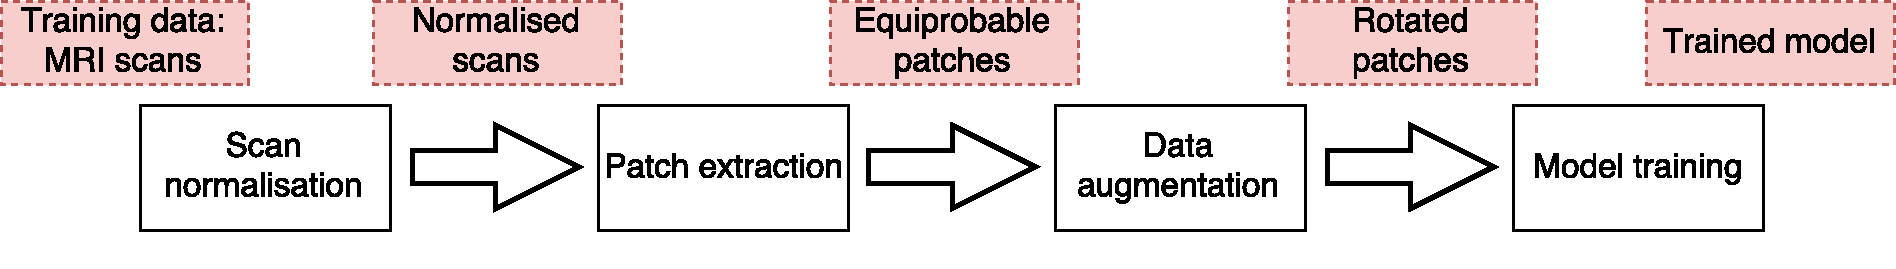
\includegraphics[width=\textwidth]{training_implementation_pipeline}
	\caption[The process of training the convolutional neural network as a pipeline]{The process of training the convolutional neural network as a pipeline. The boxes in red describe the input and outputs for each stage.}
	\label{fig:training_implementation_pipeline}
\end{figure}

\begin{figure}
	\centering
	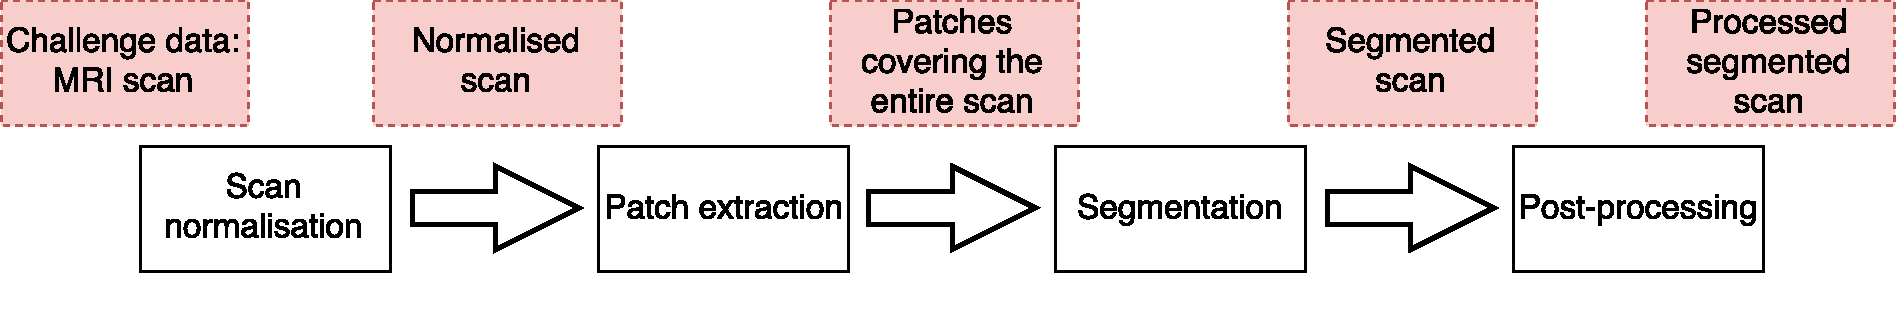
\includegraphics[width=\textwidth]{segmentation_implementation_pipeline}
	\caption[The process of segmenting an MRI scan as a pipeline]{The process of segmenting an MRI scan as a pipeline. The boxes in red describe the input and outputs for each stage.}
	\label{fig:segmentation_implementation_pipeline}
\end{figure}

I used a waterfall like approach for the implementation, building and testing the different stages independently. All stages except the scan normalisation and the post-processing are model dependent. Instead of reimplementing each stage twice, once for the model proposed by Pereira et al. and once for the model I propose, I implement each stage only once in such a way that the model-dependent aspects can be specified by parameters. This flexibility is especially important as it made it easy to experiment many different models architectures.

It is important to note that division into sequential stages provides a nice way of modularising the code base, but it is mainly conceptual. In practice, the data cannot flow in this manner because of the large amount of it. For example, in the patch extraction phase for the segmentation, it would not be possible to load all patches in memory at once. Therefore the patches are extracted and segmented slice-by-slice. The implementation of these stages is described in the next chapter.

I used git as a version control system as I was already familiar with it. The repository is stored locally and in a private GitHub repository in the cloud. I pushed the contents of the local repository to GitHub after most commits, at least once a day on which I worked on the code base. Futhermore, as an additional backup strategy I regularly back up the local repository to my external hard disk.

\section{Theoretical background}
\subsection{Artificial neural networks}
To understand how convolutional neural networks work, we first need to be familiar with ordinary neural networks. These consist of a sequence of layers of neurons, in which each neuron has a set of trainable weights that can be adjusted to change the overall function computed by the neural network. An example of the structure of such a neural network can be found in figure \ref{fig:nn_layout}. Each neuron in layer $n+1$ is connected to every neuron in layer $n$ and computes as an output
\[y = f_{act}((\sum_{i=1}^{n} y_i w_i) + b)\]
where $f_{act}$ is a non-linear, differentiable activation function and $y_i$ is the output of neuron $i$ in the previous layer. A neuron is connected to every neuron in the previous layer, which is why this layer is also called a fully-connected layer.

\begin{figure}
	\centering
	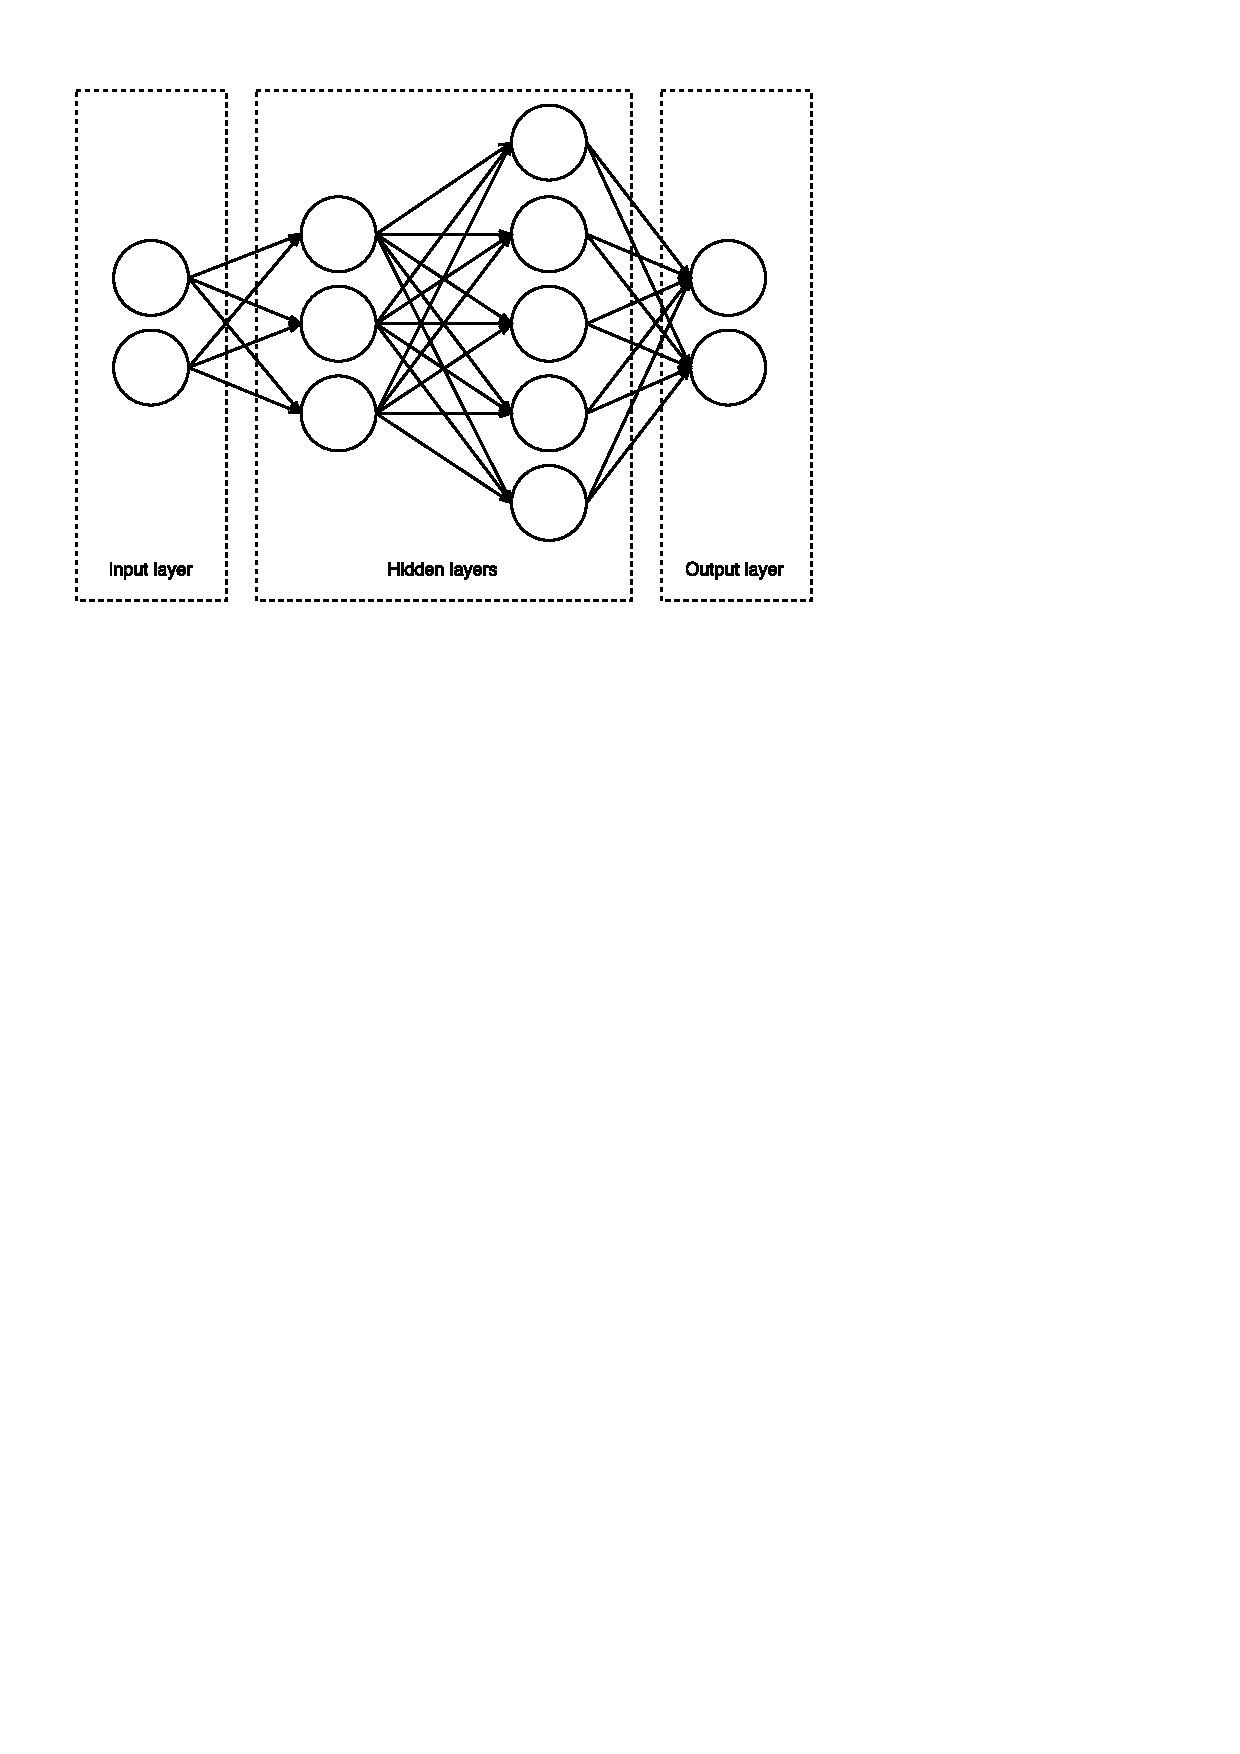
\includegraphics[scale=0.6]{nn_layout}
	\caption{Structure of a simple neural network with two hidden layers.}
	\label{fig:nn_layout}
\end{figure}

\subsubsection{Activation functions}
The most common activation functions are the Sigmoid function:
\begin{equation}
S(x) = \frac{1}{1 + e^x}
\end{equation}
the hyperbolic tangent:
\begin{equation}
	\textrm{tanh}(x)=\frac{e^x - e^{-x}}{e^x + e^{-x}}
\end{equation}
the rectifier:
\begin{equation}
\label{eq:linear_rectifier}
	f(x) = 
\begin{cases}
	0 & \text{if } x < 0\\
	x & \text{otherwise}
\end{cases}
\end{equation}
and the leaky rectifier, for $0 < \alpha < 1$:
\begin{equation}
f(x) = 
\begin{cases}
	\alpha x & \text{if } x < 0\\
	x & \text{otherwise}
\end{cases}
\end{equation}
These functions are plotted in figure \ref{fig:activation_functions}. 
\begin{figure}
	\centering 
	\setlength\figureheight{10cm}
	\setlength\figurewidth{0.8\textwidth}
	% This file was created by matplotlib2tikz v0.6.6.
\begin{tikzpicture}

\definecolor{color0}{rgb}{0,0.75,0.75}

\begin{axis}[
xmin=-2, xmax=2,
ymin=-1, ymax=2.5,
axis on top,
width=\figurewidth,
height=\figureheight,
tick pos=both,
legend entries={{sigmoid},{hyperbolic tangent},{rectifier},{leaky rectifier ($\alpha=0.333$)}},
legend style={at={(0.03,0.97)}, anchor=north west},
legend cell align={left}
]
\addplot [thick, blue]
table {%
-2 0.119202922022118
-1.99 0.120256862467751
-1.98 0.121318837891737
-1.97 0.122388886823049
-1.96 0.123467047565224
-1.95 0.124553358187416
-1.94 0.125647856515346
-1.93 0.126750580122141
-1.92 0.127861566319081
-1.91 0.128980852146236
-1.9 0.130108474362998
-1.89 0.131244469438523
-1.88 0.132388873542065
-1.87 0.133541722533212
-1.86 0.134703051952028
-1.85 0.135872897009094
-1.84 0.13705129257546
-1.83 0.138238273172494
-1.82 0.13943387296165
-1.81 0.140638125734134
-1.8 0.141851064900488
-1.79 0.143072723480081
-1.78 0.144303134090519
-1.77 0.145542328936965
-1.76 0.146790339801382
-1.75 0.14804719803169
-1.74 0.149312934530844
-1.73 0.150587579745844
-1.72 0.151871163656659
-1.71 0.153163715765086
-1.7 0.154465265083535
-1.69 0.155775840123747
-1.68 0.157095468885453
-1.67 0.158424178844956
-1.66 0.159761996943669
-1.65 0.161108949576585
-1.64 0.162465062580696
-1.63 0.163830361223359
-1.62 0.165204870190615
-1.61 0.16658861357546
-1.6 0.167981614866076
-1.59 0.169383896934019
-1.58 0.170795482022375
-1.57 0.172216391733878
-1.56 0.173646647019005
-1.55 0.17508626816404
-1.54 0.176535274779117
-1.53 0.177993685786247
-1.52 0.179461519407327
-1.51 0.180938793152142
-1.5 0.182425523806356
-1.49 0.183921727419504
-1.48 0.185427419292982
-1.47 0.186942613968046
-1.46 0.18846732521382
-1.45 0.190001566015313
-1.44 0.191545348561468
-1.43 0.193098684233217
-1.42 0.194661583591578
-1.41 0.196234056365779
-1.4 0.197816111441418
-1.39 0.199407756848669
-1.38 0.201008999750529
-1.37 0.202619846431131
-1.36 0.204240302284092
-1.35 0.205870371800947
-1.34 0.207510058559636
-1.33 0.209159365213063
-1.32 0.210818293477747
-1.31 0.212486844122539
-1.3 0.214165016957441
-1.29 0.215852810822515
-1.28 0.217550223576888
-1.27 0.219257252087872
-1.26 0.220973892220188
-1.25 0.222700138825309
-1.24 0.224435985730927
-1.23 0.226181425730546
-1.22 0.227936450573216
-1.21 0.229701050953398
-1.2 0.231475216500982
-1.19 0.233258935771457
-1.18 0.235052196236235
-1.17 0.236854984273145
-1.16 0.23866728515709
-1.15 0.240489083050889
-1.14 0.242320360996295
-1.13 0.244161100905203
-1.12 0.246011283551052
-1.11 0.24787088856043
-1.1 0.249739894404883
-1.09 0.251618278392936
-1.08 0.253506016662338
-1.07 0.255403084172524
-1.06 0.257309454697314
-1.05 0.259225100817846
-1.04 0.261149993915751
-1.03 0.26308410416658
-1.02 0.265027400533481
-1.01 0.266979850761143
-0.999999999999999 0.268941421369995
-0.989999999999999 0.270912077650694
-0.979999999999999 0.272891783658871
-0.969999999999999 0.274880502210177
-0.959999999999999 0.27687819487561
-0.949999999999999 0.278884821977137
-0.939999999999999 0.280900342583616
-0.929999999999999 0.282924714507028
-0.919999999999999 0.28495789429901
-0.909999999999999 0.286999837247718
-0.899999999999999 0.289050497374996
-0.889999999999999 0.29110982743388
-0.879999999999999 0.293177778906433
-0.869999999999999 0.295254302001909
-0.859999999999999 0.297339345655269
-0.849999999999999 0.299432857526027
-0.839999999999999 0.301534783997461
-0.829999999999999 0.303645070176166
-0.819999999999999 0.30576365989197
-0.809999999999999 0.307890495698212
-0.799999999999999 0.310025518872388
-0.789999999999999 0.31216866941716
-0.779999999999999 0.314319886061746
-0.769999999999999 0.316479106263685
-0.759999999999999 0.318646266210975
-0.749999999999999 0.320821300824607
-0.739999999999999 0.323004143761477
-0.729999999999999 0.325194727417687
-0.719999999999999 0.32739298293224
-0.709999999999999 0.329598840191132
-0.699999999999999 0.331812227831834
-0.689999999999999 0.33403307324818
-0.679999999999999 0.336261302595648
-0.669999999999999 0.338496840797048
-0.659999999999999 0.340739611548615
-0.649999999999999 0.342989537326502
-0.639999999999999 0.345246539393681
-0.629999999999999 0.347510537807256
-0.619999999999999 0.349781451426173
-0.609999999999999 0.35205919791935
-0.599999999999999 0.354343693774205
-0.589999999999999 0.356634854305599
-0.579999999999999 0.358932593665183
-0.569999999999999 0.361236824851158
-0.559999999999999 0.363547459718434
-0.549999999999999 0.3658644089892
-0.539999999999999 0.368187582263899
-0.529999999999999 0.370516888032605
-0.519999999999999 0.372852233686805
-0.509999999999999 0.375193525531571
-0.499999999999999 0.377540668798146
-0.489999999999999 0.37989356765691
-0.479999999999999 0.382252125230751
-0.469999999999999 0.384616243608818
-0.459999999999999 0.386985823860665
-0.449999999999999 0.389360766050778
-0.439999999999999 0.391740969253486
-0.429999999999999 0.39412633156824
-0.419999999999999 0.396516750135274
-0.409999999999999 0.398912121151631
-0.399999999999999 0.401312339887548
-0.389999999999999 0.403717300703212
-0.379999999999999 0.406126897065858
-0.369999999999999 0.40854102156722
-0.359999999999999 0.410959565941335
-0.349999999999999 0.41338242108267
-0.339999999999999 0.415809477064593
-0.329999999999999 0.418240623158164
-0.319999999999999 0.420675747851251
-0.309999999999998 0.423114738867954
-0.299999999999998 0.425557483188341
-0.289999999999998 0.428003867068482
-0.279999999999998 0.430453776060771
-0.269999999999998 0.432907095034546
-0.259999999999998 0.435363708196971
-0.249999999999998 0.437823499114202
-0.239999999999998 0.440286350732807
-0.229999999999998 0.442752145401445
-0.219999999999998 0.445220764892786
-0.209999999999998 0.447692090425675
-0.199999999999998 0.450166002687522
-0.189999999999998 0.452642381856911
-0.179999999999998 0.45512110762642
-0.169999999999998 0.457602059225649
-0.159999999999998 0.460085115444435
-0.149999999999998 0.462570154656251
-0.139999999999998 0.465057054841786
-0.129999999999998 0.467545693612682
-0.119999999999998 0.470035948235429
-0.109999999999998 0.472527695655407
-0.0999999999999983 0.47502081252106
-0.0899999999999983 0.4775151752082
-0.0799999999999983 0.480010659844419
-0.0699999999999983 0.482507142333611
-0.0599999999999983 0.48500449838059
-0.0499999999999983 0.48750260351579
-0.0399999999999983 0.490001333120035
-0.0299999999999983 0.49250056244938
-0.0199999999999982 0.495000166660001
-0.00999999999999823 0.497500020833125
1.77635683940025e-15 0.5
0.0100000000000016 0.502499979166875
0.0200000000000018 0.50499983334
0.030000000000002 0.507499437550621
0.0400000000000018 0.509998666879966
0.0500000000000016 0.512497396484211
0.0600000000000018 0.514995501619411
0.0700000000000021 0.51749285766639
0.0800000000000018 0.519989340155582
0.0900000000000016 0.522484824791801
0.100000000000002 0.524979187478941
0.110000000000002 0.527472304344594
0.120000000000002 0.529964051764572
0.130000000000002 0.532454306387319
0.140000000000002 0.534942945158215
0.150000000000002 0.53742984534375
0.160000000000002 0.539914884555566
0.170000000000002 0.542397940774351
0.180000000000002 0.544878892373581
0.190000000000002 0.54735761814309
0.200000000000002 0.549833997312478
0.210000000000002 0.552307909574326
0.220000000000002 0.554779235107215
0.230000000000002 0.557247854598556
0.240000000000002 0.559713649267193
0.250000000000002 0.562176500885799
0.260000000000002 0.56463629180303
0.270000000000002 0.567092904965455
0.280000000000002 0.569546223939229
0.290000000000002 0.571996132931519
0.300000000000002 0.574442516811659
0.310000000000002 0.576885261132047
0.320000000000002 0.57932425214875
0.330000000000002 0.581759376841837
0.340000000000002 0.584190522935408
0.350000000000002 0.586617578917331
0.360000000000002 0.589040434058666
0.370000000000002 0.591458978432781
0.380000000000002 0.593873102934143
0.390000000000002 0.596282699296788
0.400000000000002 0.598687660112453
0.410000000000002 0.60108787884837
0.420000000000002 0.603483249864727
0.430000000000002 0.605873668431761
0.440000000000002 0.608259030746515
0.450000000000002 0.610639233949222
0.460000000000002 0.613014176139336
0.470000000000002 0.615383756391183
0.480000000000002 0.61774787476925
0.490000000000002 0.620106432343091
0.500000000000002 0.622459331201855
0.510000000000002 0.62480647446843
0.520000000000002 0.627147766313196
0.530000000000002 0.629483111967395
0.540000000000002 0.631812417736102
0.550000000000002 0.634135591010801
0.560000000000002 0.636452540281567
0.570000000000002 0.638763175148842
0.580000000000002 0.641067406334818
0.590000000000003 0.643365145694402
0.600000000000002 0.645656306225796
0.610000000000002 0.647940802080651
0.620000000000002 0.650218548573828
0.630000000000003 0.652489462192745
0.640000000000002 0.65475346060632
0.650000000000002 0.657010462673499
0.660000000000002 0.659260388451386
0.670000000000003 0.661503159202953
0.680000000000002 0.663738697404353
0.690000000000002 0.665966926751821
0.700000000000002 0.668187772168167
0.710000000000003 0.670401159808869
0.720000000000002 0.672607017067761
0.730000000000002 0.674805272582314
0.740000000000002 0.676995856238524
0.750000000000003 0.679178699175394
0.760000000000002 0.681353733789026
0.770000000000002 0.683520893736316
0.780000000000002 0.685680113938254
0.790000000000003 0.687831330582841
0.800000000000002 0.689974481127613
0.810000000000002 0.692109504301789
0.820000000000003 0.694236340108031
0.830000000000003 0.696354929823835
0.840000000000003 0.698465216002539
0.850000000000002 0.700567142473973
0.860000000000003 0.702660654344732
0.870000000000003 0.704745697998092
0.880000000000003 0.706822221093568
0.890000000000002 0.70889017256612
0.900000000000003 0.710949502625004
0.910000000000003 0.713000162752282
0.920000000000003 0.71504210570099
0.930000000000002 0.717075285492973
0.940000000000003 0.719099657416384
0.950000000000003 0.721115178022864
0.960000000000003 0.72312180512439
0.970000000000002 0.725119497789824
0.980000000000003 0.72710821634113
0.990000000000003 0.729087922349307
1 0.731058578630005
1.01 0.733020149238858
1.02 0.734972599466519
1.03 0.736915895833421
1.04 0.73885000608425
1.05 0.740774899182154
1.06 0.742690545302686
1.07 0.744596915827477
1.08 0.746493983337663
1.09 0.748381721607065
1.1 0.750260105595118
1.11 0.752129111439571
1.12 0.753988716448949
1.13 0.755838899094798
1.14 0.757679639003705
1.15 0.759510916949112
1.16 0.761332714842911
1.17 0.763145015726856
1.18 0.764947803763765
1.19 0.766741064228543
1.2 0.768524783499018
1.21 0.770298949046602
1.22 0.772063549426784
1.23 0.773818574269454
1.24 0.775564014269074
1.25 0.777299861174692
1.26 0.779026107779813
1.27 0.780742747912129
1.28 0.782449776423113
1.29 0.784147189177486
1.3 0.785834983042559
1.31 0.787513155877461
1.32 0.789181706522253
1.33 0.790840634786937
1.34 0.792489941440365
1.35 0.794129628199053
1.36 0.795759697715909
1.37 0.79738015356887
1.38 0.798991000249471
1.39 0.800592243151332
1.4 0.802183888558582
1.41 0.803765943634221
1.42 0.805338416408423
1.43 0.806901315766784
1.44 0.808454651438533
1.45 0.809998433984687
1.46 0.811532674786181
1.47 0.813057386031954
1.48 0.814572580707018
1.49 0.816078272580496
1.5 0.817574476193644
1.51 0.819061206847858
1.52 0.820538480592674
1.53 0.822006314213754
1.54 0.823464725220884
1.55 0.824913731835961
1.56 0.826353352980995
1.57 0.827783608266123
1.58 0.829204517977626
1.59 0.830616103065982
1.6 0.832018385133925
1.61 0.833411386424541
1.62 0.834795129809386
1.63 0.836169638776642
1.64 0.837534937419304
1.65 0.838891050423415
1.66 0.840238003056331
1.67 0.841575821155045
1.68 0.842904531114548
1.69 0.844224159876253
1.7 0.845534734916466
1.71 0.846836284234914
1.72 0.848128836343341
1.73 0.849412420254156
1.74 0.850687065469157
1.75 0.851952801968311
1.76 0.853209660198618
1.77 0.854457671063035
1.78 0.855696865909482
1.79 0.85692727651992
1.8 0.858148935099513
1.81 0.859361874265866
1.82 0.86056612703835
1.83 0.861761726827506
1.84 0.862948707424541
1.85 0.864127102990906
1.86 0.865296948047972
1.87 0.866458277466788
1.88 0.867611126457935
1.89 0.868755530561477
1.9 0.869891525637003
1.91 0.871019147853765
1.92 0.872138433680919
1.93 0.87324941987786
1.94 0.874352143484655
1.95 0.875446641812584
1.96 0.876532952434776
1.97 0.877611113176952
1.98 0.878681162108264
1.99 0.87974313753225
};
\addplot [thick, green!50.0!black]
table {%
-2 -0.964027580075817
-1.99 -0.963314218604513
-1.98 -0.962586980091291
-1.97 -0.961845605369484
-1.96 -0.961089830863614
-1.95 -0.960319388531845
-1.94 -0.959534005808429
-1.93 -0.958733405546187
-1.92 -0.957917305959064
-1.91 -0.957085420564793
-1.9 -0.956237458127739
-1.89 -0.955373122601935
-1.88 -0.954492113074392
-1.87 -0.953594123708712
-1.86 -0.952678843689078
-1.85 -0.951745957164661
-1.84 -0.950795143194521
-1.83 -0.94982607569304
-1.82 -0.948838423375984
-1.81 -0.947831849707234
-1.8 -0.946806012846268
-1.79 -0.945760565596474
-1.78 -0.944695155354354
-1.77 -0.943609424059715
-1.76 -0.94250300814692
-1.75 -0.941375538497287
-1.74 -0.940226640392728
-1.73 -0.939055933470712
-1.72 -0.937863031680665
-1.71 -0.936647543241887
-1.7 -0.935409070603099
-1.69 -0.934147210403728
-1.68 -0.932861553437035
-1.67 -0.931551684615208
-1.66 -0.930217182936526
-1.65 -0.928857621454728
-1.64 -0.927472567250703
-1.63 -0.926061581406646
-1.62 -0.924624218982788
-1.61 -0.923160028996869
-1.6 -0.921668554406471
-1.59 -0.920149332094372
-1.58 -0.918601892857067
-1.57 -0.917025761396608
-1.56 -0.915420456315932
-1.55 -0.913785490117828
-1.54 -0.912120369207717
-1.53 -0.910424593900426
-1.52 -0.908697658431112
-1.51 -0.906939050970537
-1.5 -0.905148253644866
-1.49 -0.903324742560189
-1.48 -0.901467987831947
-1.47 -0.899577453619467
-1.46 -0.897652598165816
-1.45 -0.895692873843165
-1.44 -0.893697727203872
-1.43 -0.891666599037528
-1.42 -0.889598924434131
-1.41 -0.887494132853665
-1.4 -0.885351648202262
-1.39 -0.883170888915207
-1.38 -0.880951268046997
-1.37 -0.878692193368696
-1.36 -0.876393067472823
-1.35 -0.874053287886007
-1.34 -0.871672247189652
-1.33 -0.869249333148855
-1.32 -0.866783928849819
-1.31 -0.864275412846011
-1.3 -0.861723159313306
-1.29 -0.859126538214366
-1.28 -0.856484915472497
-1.27 -0.853797653155243
-1.26 -0.851064109667944
-1.25 -0.848283639957513
-1.24 -0.84545559572668
-1.23 -0.842579325658929
-1.22 -0.839654175654375
-1.21 -0.83667948907681
-1.2 -0.833654607012155
-1.19 -0.830578868538528
-1.18 -0.827451611008166
-1.17 -0.824272170341397
-1.16 -0.821039881332877
-1.15 -0.817754077970288
-1.14 -0.814414093765686
-1.13 -0.811019262099681
-1.12 -0.807568916578614
-1.11 -0.804062391404892
-1.1 -0.800499021760629
-1.09 -0.796878144204726
-1.08 -0.7931990970835
-1.07 -0.78946122095498
-1.06 -0.785663859026943
-1.05 -0.781806357608774
-1.04 -0.777888066577185
-1.03 -0.773908339855842
-1.02 -0.7698665359089
-1.01 -0.765762018248439
-0.999999999999999 -0.761594155955764
-0.989999999999999 -0.757362324216526
-0.979999999999999 -0.753065904869552
-0.969999999999999 -0.748704286969308
-0.959999999999999 -0.744276867361837
-0.949999999999999 -0.739783051274004
-0.939999999999999 -0.735222252915869
-0.929999999999999 -0.730593896095943
-0.919999999999999 -0.72589741484908
-0.909999999999999 -0.721132254076699
-0.899999999999999 -0.716297870199024
-0.889999999999999 -0.711393731818962
-0.879999999999999 -0.706419320397235
-0.869999999999999 -0.701374130938312
-0.859999999999999 -0.696257672686681
-0.849999999999999 -0.69106946983293
-0.839999999999999 -0.685809062229094
-0.829999999999999 -0.680476006112661
-0.819999999999999 -0.675069874838607
-0.809999999999999 -0.66959025961877
-0.799999999999999 -0.664036770267848
-0.789999999999999 -0.65840903595525
-0.779999999999999 -0.652706705961989
-0.769999999999999 -0.646929450441766
-0.759999999999999 -0.641076961185346
-0.749999999999999 -0.635148952387287
-0.739999999999999 -0.629145161414035
-0.729999999999999 -0.62306534957236
-0.719999999999999 -0.616909302877064
-0.709999999999999 -0.610676832816843
-0.699999999999999 -0.604367777117163
-0.689999999999999 -0.59798200049894
-0.679999999999999 -0.591519395431816
-0.669999999999999 -0.584979882880728
-0.659999999999999 -0.578363413044505
-0.649999999999999 -0.571669966085116
-0.639999999999999 -0.564899552846224
-0.629999999999999 -0.558052215559623
-0.619999999999999 -0.551128028538146
-0.609999999999999 -0.544127098853567
-0.599999999999999 -0.537049566998034
-0.589999999999999 -0.529895607527529
-0.579999999999999 -0.52266542968582
-0.569999999999999 -0.515359278007409
-0.559999999999999 -0.507977432897895
-0.549999999999999 -0.500520211190234
-0.539999999999999 -0.492987966675323
-0.529999999999999 -0.485381090605371
-0.519999999999999 -0.477700012168497
-0.509999999999999 -0.469945198933037
-0.499999999999999 -0.462117157260009
-0.489999999999999 -0.454216432682258
-0.479999999999999 -0.446243610248779
-0.469999999999999 -0.438199314832767
-0.459999999999999 -0.430084211401978
-0.449999999999999 -0.421899005250007
-0.439999999999999 -0.413644442187134
-0.429999999999999 -0.405321308689462
-0.419999999999999 -0.396930432005076
-0.409999999999999 -0.38847268021606
-0.399999999999999 -0.379948962255224
-0.389999999999999 -0.371360227876506
-0.379999999999999 -0.36270746757805
-0.369999999999999 -0.353991712477045
-0.359999999999999 -0.34521403413552
-0.349999999999999 -0.336375544336331
-0.339999999999999 -0.327477394808704
-0.329999999999999 -0.318520776902769
-0.319999999999999 -0.309506921212637
-0.309999999999998 -0.300437097147653
-0.299999999999998 -0.291312612451589
-0.289999999999998 -0.282134812669633
-0.279999999999998 -0.272905080563131
-0.269999999999998 -0.263624835472202
-0.259999999999998 -0.25429553262639
-0.249999999999998 -0.244918662403708
-0.239999999999998 -0.235495749538496
-0.229999999999998 -0.226028352278669
-0.219999999999998 -0.216518061493027
-0.209999999999998 -0.206966499729451
-0.199999999999998 -0.197375320224902
-0.189999999999998 -0.187746205868284
-0.179999999999998 -0.178080868117329
-0.169999999999998 -0.168381045870813
-0.159999999999998 -0.158648504297497
-0.149999999999998 -0.148885033623316
-0.139999999999998 -0.139092447878456
-0.129999999999998 -0.129272583606057
-0.119999999999998 -0.119427298534384
-0.109999999999998 -0.109558470214428
-0.0999999999999983 -0.0996679946249541
-0.0899999999999983 -0.0897577847471584
-0.0799999999999983 -0.0798297691111297
-0.0699999999999983 -0.0698858903164272
-0.0599999999999983 -0.0599281035291418
-0.0499999999999983 -0.0499583749578782
-0.0399999999999983 -0.0399786803111619
-0.0299999999999983 -0.0299910032388185
-0.0199999999999982 -0.0199973337599292
-0.00999999999999823 -0.00999966667999766
1.77635683940025e-15 1.77635683940025e-15
0.0100000000000016 0.00999966668000104
0.0200000000000018 0.0199973337599327
0.030000000000002 0.0299910032388222
0.0400000000000018 0.0399786803111654
0.0500000000000016 0.0499583749578816
0.0600000000000018 0.0599281035291454
0.0700000000000021 0.0698858903164311
0.0800000000000018 0.0798297691111332
0.0900000000000016 0.0897577847471617
0.100000000000002 0.0996679946249577
0.110000000000002 0.109558470214432
0.120000000000002 0.119427298534388
0.130000000000002 0.12927258360606
0.140000000000002 0.13909244787846
0.150000000000002 0.14888503362332
0.160000000000002 0.158648504297501
0.170000000000002 0.168381045870816
0.180000000000002 0.178080868117332
0.190000000000002 0.187746205868288
0.200000000000002 0.197375320224906
0.210000000000002 0.206966499729454
0.220000000000002 0.216518061493031
0.230000000000002 0.226028352278673
0.240000000000002 0.2354957495385
0.250000000000002 0.244918662403711
0.260000000000002 0.254295532626393
0.270000000000002 0.263624835472205
0.280000000000002 0.272905080563135
0.290000000000002 0.282134812669636
0.300000000000002 0.291312612451593
0.310000000000002 0.300437097147656
0.320000000000002 0.30950692121264
0.330000000000002 0.318520776902773
0.340000000000002 0.327477394808707
0.350000000000002 0.336375544336334
0.360000000000002 0.345214034135523
0.370000000000002 0.353991712477048
0.380000000000002 0.362707467578053
0.390000000000002 0.37136022787651
0.400000000000002 0.379948962255227
0.410000000000002 0.388472680216063
0.420000000000002 0.396930432005079
0.430000000000002 0.405321308689465
0.440000000000002 0.413644442187137
0.450000000000002 0.42189900525001
0.460000000000002 0.430084211401981
0.470000000000002 0.43819931483277
0.480000000000002 0.446243610248781
0.490000000000002 0.454216432682261
0.500000000000002 0.462117157260011
0.510000000000002 0.46994519893304
0.520000000000002 0.4777000121685
0.530000000000002 0.485381090605373
0.540000000000002 0.492987966675326
0.550000000000002 0.500520211190237
0.560000000000002 0.507977432897898
0.570000000000002 0.515359278007411
0.580000000000002 0.522665429685823
0.590000000000003 0.529895607527531
0.600000000000002 0.537049566998037
0.610000000000002 0.544127098853569
0.620000000000002 0.551128028538149
0.630000000000003 0.558052215559626
0.640000000000002 0.564899552846227
0.650000000000002 0.571669966085119
0.660000000000002 0.578363413044507
0.670000000000003 0.584979882880731
0.680000000000002 0.591519395431818
0.690000000000002 0.597982000498943
0.700000000000002 0.604367777117165
0.710000000000003 0.610676832816846
0.720000000000002 0.616909302877066
0.730000000000002 0.623065349572362
0.740000000000002 0.629145161414037
0.750000000000003 0.635148952387289
0.760000000000002 0.641076961185348
0.770000000000002 0.646929450441768
0.780000000000002 0.652706705961991
0.790000000000003 0.658409035955253
0.800000000000002 0.66403677026785
0.810000000000002 0.669590259618772
0.820000000000003 0.675069874838609
0.830000000000003 0.680476006112663
0.840000000000003 0.685809062229096
0.850000000000002 0.691069469832932
0.860000000000003 0.696257672686683
0.870000000000003 0.701374130938314
0.880000000000003 0.706419320397237
0.890000000000002 0.711393731818964
0.900000000000003 0.716297870199026
0.910000000000003 0.721132254076701
0.920000000000003 0.725897414849082
0.930000000000002 0.730593896095945
0.940000000000003 0.735222252915871
0.950000000000003 0.739783051274006
0.960000000000003 0.744276867361839
0.970000000000002 0.74870428696931
0.980000000000003 0.753065904869553
0.990000000000003 0.757362324216527
1 0.761594155955766
1.01 0.76576201824844
1.02 0.769866535908901
1.03 0.773908339855843
1.04 0.777888066577186
1.05 0.781806357608775
1.06 0.785663859026945
1.07 0.789461220954982
1.08 0.793199097083502
1.09 0.796878144204727
1.1 0.800499021760631
1.11 0.804062391404893
1.12 0.807568916578615
1.13 0.811019262099682
1.14 0.814414093765687
1.15 0.817754077970289
1.16 0.821039881332878
1.17 0.824272170341398
1.18 0.827451611008168
1.19 0.830578868538529
1.2 0.833654607012156
1.21 0.836679489076812
1.22 0.839654175654376
1.23 0.84257932565893
1.24 0.845455595726681
1.25 0.848283639957514
1.26 0.851064109667945
1.27 0.853797653155244
1.28 0.856484915472498
1.29 0.859126538214367
1.3 0.861723159313307
1.31 0.864275412846012
1.32 0.866783928849819
1.33 0.869249333148855
1.34 0.871672247189653
1.35 0.874053287886008
1.36 0.876393067472824
1.37 0.878692193368696
1.38 0.880951268046998
1.39 0.883170888915208
1.4 0.885351648202263
1.41 0.887494132853666
1.42 0.889598924434132
1.43 0.891666599037529
1.44 0.893697727203873
1.45 0.895692873843165
1.46 0.897652598165817
1.47 0.899577453619467
1.48 0.901467987831947
1.49 0.90332474256019
1.5 0.905148253644867
1.51 0.906939050970538
1.52 0.908697658431113
1.53 0.910424593900427
1.54 0.912120369207718
1.55 0.913785490117828
1.56 0.915420456315933
1.57 0.917025761396609
1.58 0.918601892857068
1.59 0.920149332094373
1.6 0.921668554406472
1.61 0.92316002899687
1.62 0.924624218982788
1.63 0.926061581406647
1.64 0.927472567250704
1.65 0.928857621454728
1.66 0.930217182936527
1.67 0.931551684615209
1.68 0.932861553437035
1.69 0.934147210403728
1.7 0.935409070603099
1.71 0.936647543241888
1.72 0.937863031680666
1.73 0.939055933470712
1.74 0.940226640392728
1.75 0.941375538497288
1.76 0.94250300814692
1.77 0.943609424059715
1.78 0.944695155354354
1.79 0.945760565596474
1.8 0.946806012846269
1.81 0.947831849707234
1.82 0.948838423375985
1.83 0.949826075693041
1.84 0.950795143194521
1.85 0.951745957164662
1.86 0.952678843689078
1.87 0.953594123708712
1.88 0.954492113074392
1.89 0.955373122601936
1.9 0.956237458127739
1.91 0.957085420564793
1.92 0.957917305959064
1.93 0.958733405546188
1.94 0.95953400580843
1.95 0.960319388531845
1.96 0.961089830863614
1.97 0.961845605369484
1.98 0.962586980091291
1.99 0.963314218604514
};
\addplot [thick, red]
table {%
-2 0
-1.99 0
-1.98 0
-1.97 0
-1.96 0
-1.95 0
-1.94 0
-1.93 0
-1.92 0
-1.91 0
-1.9 0
-1.89 0
-1.88 0
-1.87 0
-1.86 0
-1.85 0
-1.84 0
-1.83 0
-1.82 0
-1.81 0
-1.8 0
-1.79 0
-1.78 0
-1.77 0
-1.76 0
-1.75 0
-1.74 0
-1.73 0
-1.72 0
-1.71 0
-1.7 0
-1.69 0
-1.68 0
-1.67 0
-1.66 0
-1.65 0
-1.64 0
-1.63 0
-1.62 0
-1.61 0
-1.6 0
-1.59 0
-1.58 0
-1.57 0
-1.56 0
-1.55 0
-1.54 0
-1.53 0
-1.52 0
-1.51 0
-1.5 0
-1.49 0
-1.48 0
-1.47 0
-1.46 0
-1.45 0
-1.44 0
-1.43 0
-1.42 0
-1.41 0
-1.4 0
-1.39 0
-1.38 0
-1.37 0
-1.36 0
-1.35 0
-1.34 0
-1.33 0
-1.32 0
-1.31 0
-1.3 0
-1.29 0
-1.28 0
-1.27 0
-1.26 0
-1.25 0
-1.24 0
-1.23 0
-1.22 0
-1.21 0
-1.2 0
-1.19 0
-1.18 0
-1.17 0
-1.16 0
-1.15 0
-1.14 0
-1.13 0
-1.12 0
-1.11 0
-1.1 0
-1.09 0
-1.08 0
-1.07 0
-1.06 0
-1.05 0
-1.04 0
-1.03 0
-1.02 0
-1.01 0
-0.999999999999999 0
-0.989999999999999 0
-0.979999999999999 0
-0.969999999999999 0
-0.959999999999999 0
-0.949999999999999 0
-0.939999999999999 0
-0.929999999999999 0
-0.919999999999999 0
-0.909999999999999 0
-0.899999999999999 0
-0.889999999999999 0
-0.879999999999999 0
-0.869999999999999 0
-0.859999999999999 0
-0.849999999999999 0
-0.839999999999999 0
-0.829999999999999 0
-0.819999999999999 0
-0.809999999999999 0
-0.799999999999999 0
-0.789999999999999 0
-0.779999999999999 0
-0.769999999999999 0
-0.759999999999999 0
-0.749999999999999 0
-0.739999999999999 0
-0.729999999999999 0
-0.719999999999999 0
-0.709999999999999 0
-0.699999999999999 0
-0.689999999999999 0
-0.679999999999999 0
-0.669999999999999 0
-0.659999999999999 0
-0.649999999999999 0
-0.639999999999999 0
-0.629999999999999 0
-0.619999999999999 0
-0.609999999999999 0
-0.599999999999999 0
-0.589999999999999 0
-0.579999999999999 0
-0.569999999999999 0
-0.559999999999999 0
-0.549999999999999 0
-0.539999999999999 0
-0.529999999999999 0
-0.519999999999999 0
-0.509999999999999 0
-0.499999999999999 0
-0.489999999999999 0
-0.479999999999999 0
-0.469999999999999 0
-0.459999999999999 0
-0.449999999999999 0
-0.439999999999999 0
-0.429999999999999 0
-0.419999999999999 0
-0.409999999999999 0
-0.399999999999999 0
-0.389999999999999 0
-0.379999999999999 0
-0.369999999999999 0
-0.359999999999999 0
-0.349999999999999 0
-0.339999999999999 0
-0.329999999999999 0
-0.319999999999999 0
-0.309999999999998 0
-0.299999999999998 0
-0.289999999999998 0
-0.279999999999998 0
-0.269999999999998 0
-0.259999999999998 0
-0.249999999999998 0
-0.239999999999998 0
-0.229999999999998 0
-0.219999999999998 0
-0.209999999999998 0
-0.199999999999998 0
-0.189999999999998 0
-0.179999999999998 0
-0.169999999999998 0
-0.159999999999998 0
-0.149999999999998 0
-0.139999999999998 0
-0.129999999999998 0
-0.119999999999998 0
-0.109999999999998 0
-0.0999999999999983 0
-0.0899999999999983 0
-0.0799999999999983 0
-0.0699999999999983 0
-0.0599999999999983 0
-0.0499999999999983 0
-0.0399999999999983 0
-0.0299999999999983 0
-0.0199999999999982 0
-0.00999999999999823 0
1.77635683940025e-15 0
0.0100000000000016 0
0.0200000000000018 0.00500000000000179
0.030000000000002 0.015000000000002
0.0400000000000018 0.0250000000000018
0.0500000000000016 0.0350000000000016
0.0600000000000018 0.0450000000000018
0.0700000000000021 0.0550000000000021
0.0800000000000018 0.0650000000000018
0.0900000000000016 0.0750000000000016
0.100000000000002 0.0850000000000019
0.110000000000002 0.0950000000000021
0.120000000000002 0.105000000000002
0.130000000000002 0.115000000000002
0.140000000000002 0.125000000000002
0.150000000000002 0.135000000000002
0.160000000000002 0.145000000000002
0.170000000000002 0.155000000000002
0.180000000000002 0.165000000000002
0.190000000000002 0.175000000000002
0.200000000000002 0.185000000000002
0.210000000000002 0.195000000000002
0.220000000000002 0.205000000000002
0.230000000000002 0.215000000000002
0.240000000000002 0.225000000000002
0.250000000000002 0.235000000000002
0.260000000000002 0.245000000000002
0.270000000000002 0.255000000000002
0.280000000000002 0.265000000000002
0.290000000000002 0.275000000000002
0.300000000000002 0.285000000000002
0.310000000000002 0.295000000000002
0.320000000000002 0.305000000000002
0.330000000000002 0.315000000000002
0.340000000000002 0.325000000000002
0.350000000000002 0.335000000000002
0.360000000000002 0.345000000000002
0.370000000000002 0.355000000000002
0.380000000000002 0.365000000000002
0.390000000000002 0.375000000000002
0.400000000000002 0.385000000000002
0.410000000000002 0.395000000000002
0.420000000000002 0.405000000000002
0.430000000000002 0.415000000000002
0.440000000000002 0.425000000000002
0.450000000000002 0.435000000000002
0.460000000000002 0.445000000000002
0.470000000000002 0.455000000000002
0.480000000000002 0.465000000000002
0.490000000000002 0.475000000000002
0.500000000000002 0.485000000000002
0.510000000000002 0.495000000000002
0.520000000000002 0.505000000000002
0.530000000000002 0.515000000000002
0.540000000000002 0.525000000000002
0.550000000000002 0.535000000000002
0.560000000000002 0.545000000000002
0.570000000000002 0.555000000000002
0.580000000000002 0.565000000000002
0.590000000000003 0.575000000000003
0.600000000000002 0.585000000000002
0.610000000000002 0.595000000000002
0.620000000000002 0.605000000000002
0.630000000000003 0.615000000000003
0.640000000000002 0.625000000000002
0.650000000000002 0.635000000000002
0.660000000000002 0.645000000000002
0.670000000000003 0.655000000000003
0.680000000000002 0.665000000000002
0.690000000000002 0.675000000000002
0.700000000000002 0.685000000000002
0.710000000000003 0.695000000000003
0.720000000000002 0.705000000000002
0.730000000000002 0.715000000000002
0.740000000000002 0.725000000000002
0.750000000000003 0.735000000000003
0.760000000000002 0.745000000000002
0.770000000000002 0.755000000000002
0.780000000000002 0.765000000000002
0.790000000000003 0.775000000000003
0.800000000000002 0.785000000000002
0.810000000000002 0.795000000000002
0.820000000000003 0.805000000000002
0.830000000000003 0.815000000000003
0.840000000000003 0.825000000000003
0.850000000000002 0.835000000000002
0.860000000000003 0.845000000000003
0.870000000000003 0.855000000000003
0.880000000000003 0.865000000000003
0.890000000000002 0.875000000000002
0.900000000000003 0.885000000000003
0.910000000000003 0.895000000000003
0.920000000000003 0.905000000000003
0.930000000000002 0.915000000000002
0.940000000000003 0.925000000000003
0.950000000000003 0.935000000000003
0.960000000000003 0.945000000000003
0.970000000000002 0.955000000000002
0.980000000000003 0.965000000000003
0.990000000000003 0.975000000000003
1 0.985000000000003
1.01 0.995000000000002
1.02 1.005
1.03 1.015
1.04 1.025
1.05 1.035
1.06 1.045
1.07 1.055
1.08 1.065
1.09 1.075
1.1 1.085
1.11 1.095
1.12 1.105
1.13 1.115
1.14 1.125
1.15 1.135
1.16 1.145
1.17 1.155
1.18 1.165
1.19 1.175
1.2 1.185
1.21 1.195
1.22 1.205
1.23 1.215
1.24 1.225
1.25 1.235
1.26 1.245
1.27 1.255
1.28 1.265
1.29 1.275
1.3 1.285
1.31 1.295
1.32 1.305
1.33 1.315
1.34 1.325
1.35 1.335
1.36 1.345
1.37 1.355
1.38 1.365
1.39 1.375
1.4 1.385
1.41 1.395
1.42 1.405
1.43 1.415
1.44 1.425
1.45 1.435
1.46 1.445
1.47 1.455
1.48 1.465
1.49 1.475
1.5 1.485
1.51 1.495
1.52 1.505
1.53 1.515
1.54 1.525
1.55 1.535
1.56 1.545
1.57 1.555
1.58 1.565
1.59 1.575
1.6 1.585
1.61 1.595
1.62 1.605
1.63 1.615
1.64 1.625
1.65 1.635
1.66 1.645
1.67 1.655
1.68 1.665
1.69 1.675
1.7 1.685
1.71 1.695
1.72 1.705
1.73 1.715
1.74 1.725
1.75 1.735
1.76 1.745
1.77 1.755
1.78 1.765
1.79 1.775
1.8 1.785
1.81 1.795
1.82 1.805
1.83 1.815
1.84 1.825
1.85 1.835
1.86 1.845
1.87 1.855
1.88 1.865
1.89 1.875
1.9 1.885
1.91 1.895
1.92 1.905
1.93 1.915
1.94 1.925
1.95 1.935
1.96 1.945
1.97 1.955
1.98 1.965
1.99 1.975
};
\addplot [thick, color0]
table {%
-2 -0.666
-1.99 -0.66267
-1.98 -0.65934
-1.97 -0.65601
-1.96 -0.65268
-1.95 -0.64935
-1.94 -0.64602
-1.93 -0.64269
-1.92 -0.63936
-1.91 -0.63603
-1.9 -0.6327
-1.89 -0.62937
-1.88 -0.62604
-1.87 -0.62271
-1.86 -0.61938
-1.85 -0.61605
-1.84 -0.61272
-1.83 -0.60939
-1.82 -0.60606
-1.81 -0.60273
-1.8 -0.5994
-1.79 -0.59607
-1.78 -0.59274
-1.77 -0.58941
-1.76 -0.58608
-1.75 -0.58275
-1.74 -0.57942
-1.73 -0.57609
-1.72 -0.57276
-1.71 -0.56943
-1.7 -0.5661
-1.69 -0.56277
-1.68 -0.55944
-1.67 -0.55611
-1.66 -0.55278
-1.65 -0.54945
-1.64 -0.54612
-1.63 -0.54279
-1.62 -0.53946
-1.61 -0.53613
-1.6 -0.5328
-1.59 -0.52947
-1.58 -0.52614
-1.57 -0.52281
-1.56 -0.51948
-1.55 -0.51615
-1.54 -0.51282
-1.53 -0.50949
-1.52 -0.50616
-1.51 -0.50283
-1.5 -0.4995
-1.49 -0.49617
-1.48 -0.49284
-1.47 -0.48951
-1.46 -0.48618
-1.45 -0.48285
-1.44 -0.47952
-1.43 -0.47619
-1.42 -0.47286
-1.41 -0.46953
-1.4 -0.4662
-1.39 -0.46287
-1.38 -0.45954
-1.37 -0.45621
-1.36 -0.45288
-1.35 -0.44955
-1.34 -0.44622
-1.33 -0.44289
-1.32 -0.43956
-1.31 -0.43623
-1.3 -0.4329
-1.29 -0.42957
-1.28 -0.42624
-1.27 -0.42291
-1.26 -0.41958
-1.25 -0.41625
-1.24 -0.41292
-1.23 -0.40959
-1.22 -0.40626
-1.21 -0.40293
-1.2 -0.3996
-1.19 -0.39627
-1.18 -0.39294
-1.17 -0.38961
-1.16 -0.38628
-1.15 -0.38295
-1.14 -0.37962
-1.13 -0.37629
-1.12 -0.37296
-1.11 -0.36963
-1.1 -0.3663
-1.09 -0.36297
-1.08 -0.35964
-1.07 -0.35631
-1.06 -0.35298
-1.05 -0.34965
-1.04 -0.34632
-1.03 -0.34299
-1.02 -0.33966
-1.01 -0.33633
-0.999999999999999 -0.333
-0.989999999999999 -0.32967
-0.979999999999999 -0.32634
-0.969999999999999 -0.32301
-0.959999999999999 -0.31968
-0.949999999999999 -0.31635
-0.939999999999999 -0.31302
-0.929999999999999 -0.30969
-0.919999999999999 -0.30636
-0.909999999999999 -0.30303
-0.899999999999999 -0.2997
-0.889999999999999 -0.29637
-0.879999999999999 -0.29304
-0.869999999999999 -0.28971
-0.859999999999999 -0.28638
-0.849999999999999 -0.28305
-0.839999999999999 -0.27972
-0.829999999999999 -0.27639
-0.819999999999999 -0.27306
-0.809999999999999 -0.26973
-0.799999999999999 -0.2664
-0.789999999999999 -0.26307
-0.779999999999999 -0.25974
-0.769999999999999 -0.25641
-0.759999999999999 -0.25308
-0.749999999999999 -0.24975
-0.739999999999999 -0.24642
-0.729999999999999 -0.24309
-0.719999999999999 -0.23976
-0.709999999999999 -0.23643
-0.699999999999999 -0.2331
-0.689999999999999 -0.22977
-0.679999999999999 -0.22644
-0.669999999999999 -0.22311
-0.659999999999999 -0.21978
-0.649999999999999 -0.21645
-0.639999999999999 -0.21312
-0.629999999999999 -0.20979
-0.619999999999999 -0.20646
-0.609999999999999 -0.20313
-0.599999999999999 -0.1998
-0.589999999999999 -0.19647
-0.579999999999999 -0.19314
-0.569999999999999 -0.18981
-0.559999999999999 -0.18648
-0.549999999999999 -0.18315
-0.539999999999999 -0.17982
-0.529999999999999 -0.17649
-0.519999999999999 -0.17316
-0.509999999999999 -0.16983
-0.499999999999999 -0.1665
-0.489999999999999 -0.16317
-0.479999999999999 -0.15984
-0.469999999999999 -0.15651
-0.459999999999999 -0.15318
-0.449999999999999 -0.14985
-0.439999999999999 -0.14652
-0.429999999999999 -0.14319
-0.419999999999999 -0.13986
-0.409999999999999 -0.13653
-0.399999999999999 -0.1332
-0.389999999999999 -0.12987
-0.379999999999999 -0.12654
-0.369999999999999 -0.12321
-0.359999999999999 -0.11988
-0.349999999999999 -0.11655
-0.339999999999999 -0.11322
-0.329999999999999 -0.10989
-0.319999999999999 -0.10656
-0.309999999999998 -0.10323
-0.299999999999998 -0.0998999999999995
-0.289999999999998 -0.0965699999999995
-0.279999999999998 -0.0932399999999995
-0.269999999999998 -0.0899099999999995
-0.259999999999998 -0.0865799999999995
-0.249999999999998 -0.0832499999999995
-0.239999999999998 -0.0799199999999995
-0.229999999999998 -0.0765899999999995
-0.219999999999998 -0.0732599999999995
-0.209999999999998 -0.0699299999999995
-0.199999999999998 -0.0665999999999995
-0.189999999999998 -0.0632699999999995
-0.179999999999998 -0.0599399999999995
-0.169999999999998 -0.0566099999999995
-0.159999999999998 -0.0532799999999995
-0.149999999999998 -0.0499499999999995
-0.139999999999998 -0.0466199999999995
-0.129999999999998 -0.0432899999999994
-0.119999999999998 -0.0399599999999994
-0.109999999999998 -0.0366299999999994
-0.0999999999999983 -0.0332999999999994
-0.0899999999999983 -0.0299699999999994
-0.0799999999999983 -0.0266399999999994
-0.0699999999999983 -0.0233099999999994
-0.0599999999999983 -0.0199799999999994
-0.0499999999999983 -0.0166499999999994
-0.0399999999999983 -0.0133199999999994
-0.0299999999999983 -0.00998999999999942
-0.0199999999999982 -0.00665999999999941
-0.00999999999999823 -0.00332999999999941
1.77635683940025e-15 0.0150000000000018
0.0100000000000016 0.0250000000000016
0.0200000000000018 0.0350000000000018
0.030000000000002 0.045000000000002
0.0400000000000018 0.0550000000000018
0.0500000000000016 0.0650000000000016
0.0600000000000018 0.0750000000000018
0.0700000000000021 0.0850000000000021
0.0800000000000018 0.0950000000000018
0.0900000000000016 0.105000000000002
0.100000000000002 0.115000000000002
0.110000000000002 0.125000000000002
0.120000000000002 0.135000000000002
0.130000000000002 0.145000000000002
0.140000000000002 0.155000000000002
0.150000000000002 0.165000000000002
0.160000000000002 0.175000000000002
0.170000000000002 0.185000000000002
0.180000000000002 0.195000000000002
0.190000000000002 0.205000000000002
0.200000000000002 0.215000000000002
0.210000000000002 0.225000000000002
0.220000000000002 0.235000000000002
0.230000000000002 0.245000000000002
0.240000000000002 0.255000000000002
0.250000000000002 0.265000000000002
0.260000000000002 0.275000000000002
0.270000000000002 0.285000000000002
0.280000000000002 0.295000000000002
0.290000000000002 0.305000000000002
0.300000000000002 0.315000000000002
0.310000000000002 0.325000000000002
0.320000000000002 0.335000000000002
0.330000000000002 0.345000000000002
0.340000000000002 0.355000000000002
0.350000000000002 0.365000000000002
0.360000000000002 0.375000000000002
0.370000000000002 0.385000000000002
0.380000000000002 0.395000000000002
0.390000000000002 0.405000000000002
0.400000000000002 0.415000000000002
0.410000000000002 0.425000000000002
0.420000000000002 0.435000000000002
0.430000000000002 0.445000000000002
0.440000000000002 0.455000000000002
0.450000000000002 0.465000000000002
0.460000000000002 0.475000000000002
0.470000000000002 0.485000000000002
0.480000000000002 0.495000000000002
0.490000000000002 0.505000000000002
0.500000000000002 0.515000000000002
0.510000000000002 0.525000000000002
0.520000000000002 0.535000000000002
0.530000000000002 0.545000000000002
0.540000000000002 0.555000000000002
0.550000000000002 0.565000000000003
0.560000000000002 0.575000000000002
0.570000000000002 0.585000000000002
0.580000000000002 0.595000000000002
0.590000000000003 0.605000000000003
0.600000000000002 0.615000000000002
0.610000000000002 0.625000000000002
0.620000000000002 0.635000000000002
0.630000000000003 0.645000000000003
0.640000000000002 0.655000000000002
0.650000000000002 0.665000000000002
0.660000000000002 0.675000000000002
0.670000000000003 0.685000000000003
0.680000000000002 0.695000000000002
0.690000000000002 0.705000000000002
0.700000000000002 0.715000000000002
0.710000000000003 0.725000000000003
0.720000000000002 0.735000000000002
0.730000000000002 0.745000000000002
0.740000000000002 0.755000000000002
0.750000000000003 0.765000000000003
0.760000000000002 0.775000000000002
0.770000000000002 0.785000000000002
0.780000000000002 0.795000000000002
0.790000000000003 0.805000000000003
0.800000000000002 0.815000000000003
0.810000000000002 0.825000000000002
0.820000000000003 0.835000000000003
0.830000000000003 0.845000000000003
0.840000000000003 0.855000000000003
0.850000000000002 0.865000000000002
0.860000000000003 0.875000000000003
0.870000000000003 0.885000000000003
0.880000000000003 0.895000000000003
0.890000000000002 0.905000000000002
0.900000000000003 0.915000000000003
0.910000000000003 0.925000000000003
0.920000000000003 0.935000000000003
0.930000000000002 0.945000000000002
0.940000000000003 0.955000000000003
0.950000000000003 0.965000000000003
0.960000000000003 0.975000000000003
0.970000000000002 0.985000000000002
0.980000000000003 0.995000000000003
0.990000000000003 1.005
1 1.015
1.01 1.025
1.02 1.035
1.03 1.045
1.04 1.055
1.05 1.065
1.06 1.075
1.07 1.085
1.08 1.095
1.09 1.105
1.1 1.115
1.11 1.125
1.12 1.135
1.13 1.145
1.14 1.155
1.15 1.165
1.16 1.175
1.17 1.185
1.18 1.195
1.19 1.205
1.2 1.215
1.21 1.225
1.22 1.235
1.23 1.245
1.24 1.255
1.25 1.265
1.26 1.275
1.27 1.285
1.28 1.295
1.29 1.305
1.3 1.315
1.31 1.325
1.32 1.335
1.33 1.345
1.34 1.355
1.35 1.365
1.36 1.375
1.37 1.385
1.38 1.395
1.39 1.405
1.4 1.415
1.41 1.425
1.42 1.435
1.43 1.445
1.44 1.455
1.45 1.465
1.46 1.475
1.47 1.485
1.48 1.495
1.49 1.505
1.5 1.515
1.51 1.525
1.52 1.535
1.53 1.545
1.54 1.555
1.55 1.565
1.56 1.575
1.57 1.585
1.58 1.595
1.59 1.605
1.6 1.615
1.61 1.625
1.62 1.635
1.63 1.645
1.64 1.655
1.65 1.665
1.66 1.675
1.67 1.685
1.68 1.695
1.69 1.705
1.7 1.715
1.71 1.725
1.72 1.735
1.73 1.745
1.74 1.755
1.75 1.765
1.76 1.775
1.77 1.785
1.78 1.795
1.79 1.805
1.8 1.815
1.81 1.825
1.82 1.835
1.83 1.845
1.84 1.855
1.85 1.865
1.86 1.875
1.87 1.885
1.88 1.895
1.89 1.905
1.9 1.915
1.91 1.925
1.92 1.935
1.93 1.945
1.94 1.955
1.95 1.965
1.96 1.975
1.97 1.985
1.98 1.995
1.99 2.005
};
\end{axis}

\end{tikzpicture}
	\caption{Plot of the activation functions.}
	\label{fig:activation_functions}
\end{figure}
Historically, the hyperbolic tangent function or the sigmoid function have been used as activation functions. However, the magnitude of the gradients of these two activation functions is always below 1. This causes a numerical issue for deeper networks, as the gradients for each layer are multiplied together during the backpropagation algorithm. This is known as the vanishing gradient problem \cite{vanishing_gradients} and is the reason why it is nowadays preferred to use the rectifier or the leaky rectifier functions, especially with deeper architectures.

In a classification problem, the output layer usually consist of $K$ nodes, one for each class. Using a softmax activation function for the last layer, we can interpret the value at each node as the probability that the input belongs to this class.  More formally, in a of a network with parameters $\theta$, we can view the output of node $k$ when presented with input $x^{(i)}$ as the probability $P(y_{\text{pred}}^{(i)} = k \mid x^{(i)};\theta)$. The softmax activation computes for each output $k$
\begin{equation}
	\sigma(\mathbf{x})_k = \frac{e^{\mathbf{x}_k}}{\sum_{j=1}^{K}e^{\mathbf{x}_j}}
\end{equation}
where $\mathbf{x}$ is the vector consisting of all outputs from the previous layer. The output value of each neuron will range between 0 and 1 and the sum of all outputs will be 1, hence we can indeed interpret the output as a probability distribution.

\subsubsection{Loss function}
Now, that we have defined what the network computes for each input, we need to measure how well our network approximates our training data. A loss function is therefore introduced. Since the aim of the network is to classify the central pixel(s) of the patch, we use the categorical cross-entropy loss function
\begin{equation}
	\label{eq:loss}
	\mathcal{L}(\theta) = 
	\frac{1}{m}\Big[\sum_{i=1}^m \sum_{j=1}^k\mathbbm{1}[y^{(i)} = k]\log(P(y_{\text{pred}}^{(i)}=k \mid x^{(i)};\theta))\Big]
\end{equation}
where $\mathbbm{1}$ is the indicator function and $P(y_{\text{pred}}^{(i)}=k \mid x^{(i)};\theta)$ is the probability computed by the neural network with weights $\theta$ that input vector $x^{(i)}$ belongs to class $k$.

\subsubsection{Optimisation}
We now aim to minimise this loss function. This is done by using the stochastic gradient descent algorithm. First, we need to compute the gradient $\frac{d\mathcal{L}(\theta)}{d\theta}$, so that we can apply gradient descent and update our weight vector to
\begin{equation}
	\theta = \theta - \epsilon \frac{d\mathcal{L}(\theta)}{d\theta}
\end{equation}
where $\epsilon$ is the learning rate, a small positive value.

Since every basic operation used in the neural network is differentiable, the entire network will also be differentiable, which in turn makes it possible to calculate the gradient of a differentiable loss function with respect to the weights in the network by repeatedly applying the chain rule. This process is called the backpropagation algorithm.

The loss functions, as described in equation \ref{eq:loss} is computed using the entire training data set $\mathbb{X} = \{(x^{(1)},y^{(1)}), ...,(x^{(m)},y^{(m)})\}$. In the case of deep learning where it is usual to have a very large training data set, this would be very memory costly and slow down the training phase unnecessarily. A solution to this problem is to use stochastic gradient descent instead where the training data is split sequentially in batches. The loss and corresponding gradient updates are then computed individually for each batch.

\subsubsection{Momentum}
An optimisation used to speed up the training process is momentum update. Minimising the loss function can be interpreted as moving a small particle down a hilly terrain in the hyper-dimensional space defined by the loss function. Since the gradient is related to the force experienced by that particle, this suggest that the gradient should only influence the velocity vector and not the position directly. This leads to the velocity update
\begin{equation}
	v = \mu  v - \epsilon \frac{d\mathcal{L}(\theta)}{d\theta}
\end{equation}
where $\mu$ is the momentum, typically set to 0.9. We then update our weights by simply adding the velocity to the current value.
\begin{equation}
	\theta = \theta + v
\end{equation}

Typically a slightly different version, called the Nesterov momentum, is used as it has been shown to work better in practice \cite{nesterov_momentum}.

\subsection{Convolutional neural networks}
Convolutional neural networks make the explicit assumption that the inputs are images. This allows us to take advantage of some properties of images to make the forward function more effective and greatly reduce the number of weights in our network. 

A typical convolutional network constists of three types of layers:
\begin{enumerate}
	\item \textbf{Fully-connected layers}: These are identical to the layers in ordinary neural networks as introduced earlier.
	\item \textbf{Convolutional layers}: A convolutional layer is three-dimensional, consisting of a width, height and depth. The parameters of a layer define a set of learnable filters, each spatially small along the width and height of the layer but with the depth equal to the depth of the input volume. Each filter in the layer is convolved with the input and computes the dot product at each point. The result is of this operation is a two-dimensional activation map, which has translational invariance, as the filter is convolved with the entire input and thus the same feature is detected independently of location. The computation done by such a filter in shown in figure \ref{fig:conv_example}. Finally, the two-dimensional activation maps are stacked along the depth axis to produce the output volume.
	
	\begin{figure}
		\centering
		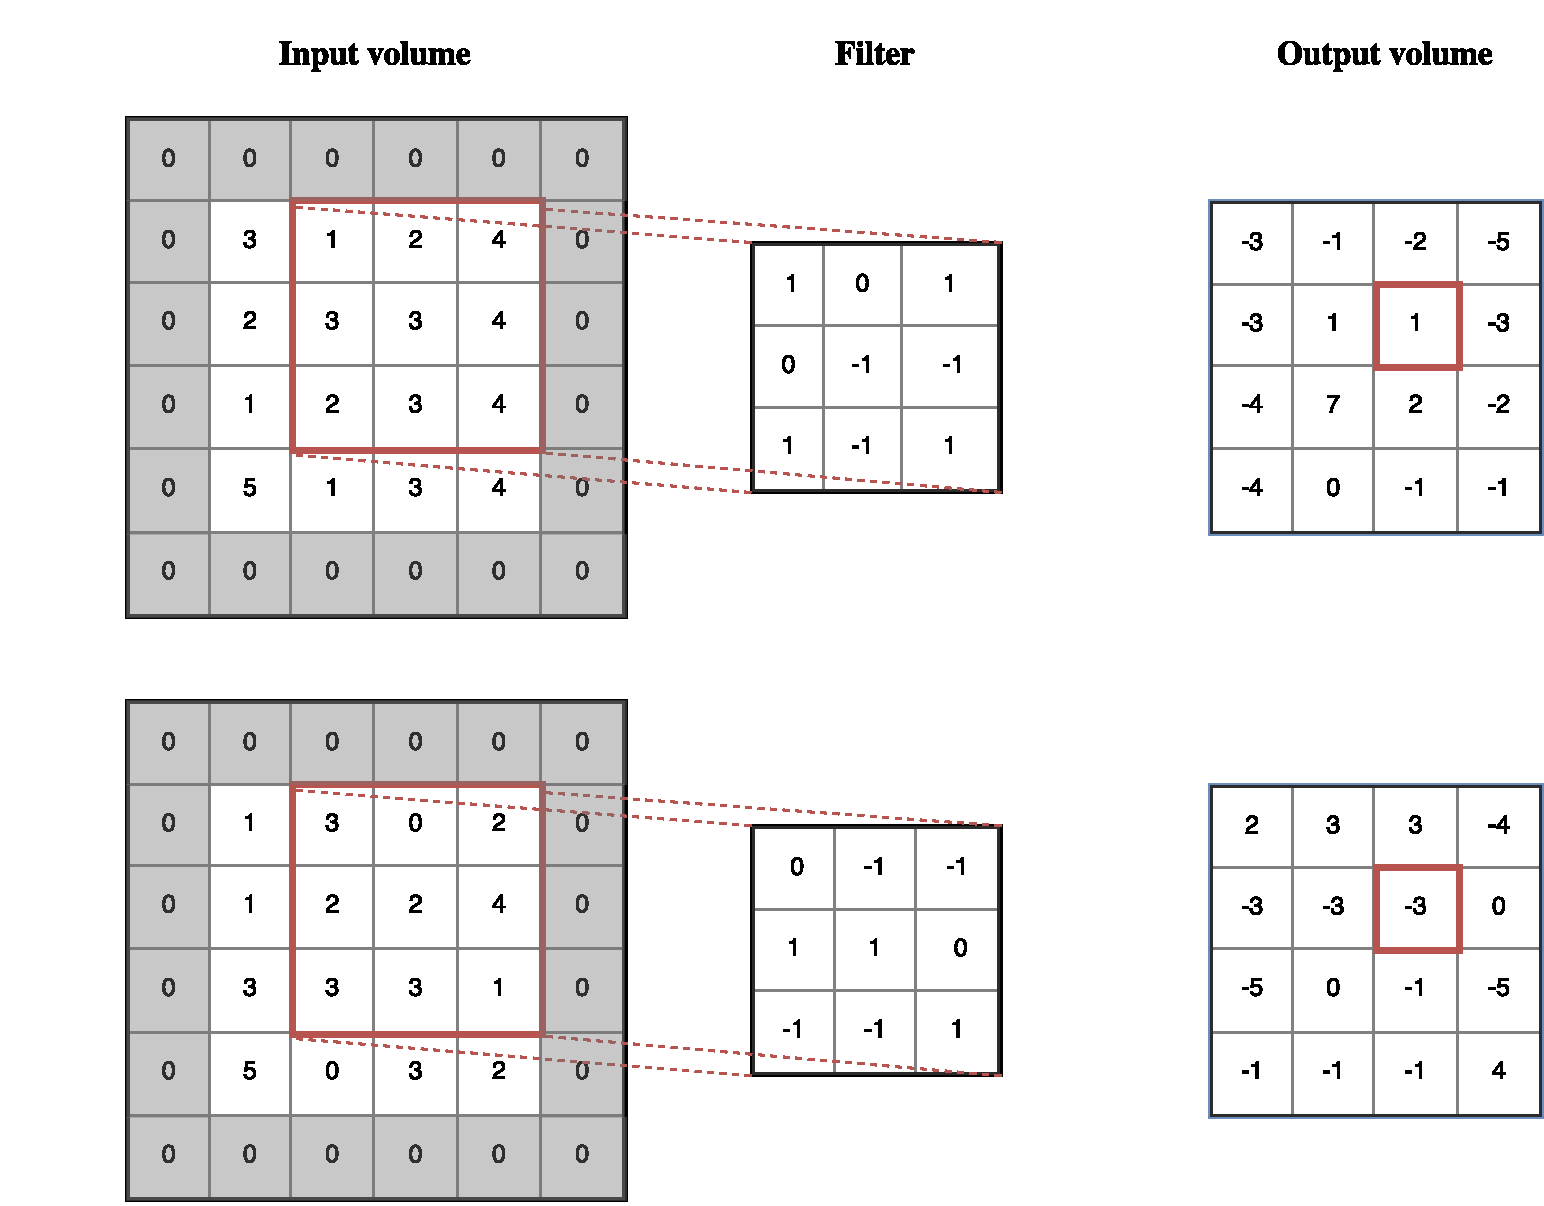
\includegraphics[scale=0.6]{conv_example}
		\caption[Example computation done by a 3x3 filter in a convolutional layer]{Example computation done by a 3x3 filter in a convolutional layer. Both the stride and the padding are 1, so as to keep the output dimensions identical. The output at depth 0 for the marked element is $1 \cdot 1 + 2 \cdot 0 + 4 \cdot 1 + 3 \cdot 0 + 3 \cdot -1 + 4 \cdot -1 + 2 \cdot 1 + 3 \cdot -1 + 4 \cdot 1 = 1$ and similarly at depth 1 the output for that element is -3.}
		\label{fig:conv_example}
	\end{figure}

	This connectivity pattern is inspired by the organization of the animal visual cortex. Individual neurons respond to stimuli in a small region of space known as the \textbf{receptive field}. Every value in an activation map can then be interpreted as the output of a neuron whose receptive field is the width and height of the filter and who shares its weights with all its neighbours to the left and right spatially.

	The size of the output volume is determined by the following hyperparameters:
	\begin{enumerate}
		\item The \textbf{depth} corresponds to the number of filters in the layer and is therefore equal to the depth of the output volume.
		\item The \textbf{stride} which determines by how many pixels the filter is moved during each step ofthe convolution. When the stride is greater than 1 the output will be smaller than the input.
		\item The \textbf{padding} determines with how many zeros we pad the input width and height. This is particularly useful when we want to preserve the input dimensions.
	\end{enumerate}
	
	\item \textbf{Pooling layers}: The function of the pooling layer is to reduce the spatial size of the input layer in order to reduce the number of parameters and computation in the network. The most common pooling layer implementation is the \textbf{max-pooling} which just convolves a two-dimensional maximum operator of a given size, typically 2x2. The \textbf{stride} again determines the step size.

\end{enumerate}

A convolutional neural network typically consists of a sequence of these layers, starting with pairs of convolutional layers and max--pooling layers. The idea is that each one of these pairs of convolutional and pooling layers can learn more and more abstract features using the features learned by the previous layer. For example, the first pair might learn to recognise edges, the second layer shapes, etc.. The last few layers of the network consist entirely of fully-connected layers. These learn how to classify the data using the features learned by the convolutional and max pooling layers.

\subsection{The overfitting problem}
A common problem that arises with neural networks models is \textbf{overfitting}. This occurs when the model is not able to generalise on previously unseen data and instead just memorises the training data. Due to the large number of weights in deep convolutional neural networks, these are particularly prone to overfitting. Many techniques and heuristics have been developed in order to help prevent this; in my project I have used three of them: \textbf{L2 weight regularisation}, \textbf{Dropout} and \textbf{Batch Normalisation}, which I discuss below.

\subsubsection{\textbf{L2} weight regularisation}
The L2 regularisation prevents individual parameters to grow without bounds, instead making the network use all its parameters, which has the effect of preventing the model from just memorising the data\footnote{\url{http://cs231n.github.io/neural-networks-2/\#reg}}. This is achieved by adding a regularisation penalty to the loss function. There are many different regularisation costs one could use, the most common ones are the L2 and L1 normalisation. In my project, I used the L2 normalisation which computes the sum of the squares of every parameter:
\begin{equation}
	R(\theta) = \sum_{k}^{} \sum_{l}^{} \theta_{k,l}^2
\end{equation} 
where $\theta$ is the weight matrix that includes all weights, including biases.
The loss function that we aim to minimise thus becomes
\begin{equation}
	\mathcal{L}(\theta) = \mathcal{L}_{data}(\theta) + R(\theta) 
\end{equation}
where $\mathcal{L}_{data}(\theta)$ is the data loss, defined in equation \ref{eq:loss}. 

\subsubsection{Dropout}
A more recent technique, developed for deep neural networks is Dropout \cite{dropout}. When Dropout is used, the network randomly drops some neurons during the training phase. This forces the network to distribute the computation on all neurons evenly, which prevents the network from overfitting. The computation done by a single neuron thus becomes
\begin{equation}
\begin{split}
	\textbf{r} & \sim \text{Bernoulli}_n(p) \\
	y & = f_{act}((\sum_{i=1}^{n} r_i y_i w_i) + b)
\end{split}
\end{equation}
where $\textbf{r}$ is a vector of $n$ independent Bernoulli random variables each with probability $p$ of being one, that is $P(r_i = 1) = p$ and $P(r_i = 0) = 1 - p$ for each $r_i$. This is done at every layer and therefore amounts to sampling a sub-network from a larger network. 

At test time dropout is not applied. Thus, the network weights have to be scaled by a factor $p$ to compensate for the extra inputs at each layer. The back-propagation algorithm remains unchanged for the sub-network and can therefore be applied in the learning phase.

In practice, it is common to apply Dropout only to the fully connected layers and not to the convolutional layers, as it has been shown to produce better results. As I will show later, this is also what was done by Pereira et al. \cite{pereira}.

\subsubsection{Batch Normalisation}
The final regularisation technique used is Batch Normalisation \cite{batch_normalization}. As this technique is more recent than the paper published by Pereira et al., it was not used in their method. However, in the second phase of my project I experiment with a different architecture in which I used Batch Normalisation to prevent overfitting.

The important realisation is that the distribution of the inputs to each layer change as the weights of the network are changed. This phenomenon is called \textit{internal covariance shift}. The training of the neural network is slowed down by this because each layer has to continuously adapt to this change in the distribution of its inputs. By fixing the distribution of these inputs the network is able to learn faster and is less prone to overfitting. Similarly to how the inputs to the network are often normalised to have mean 0 and variance 1, it would be beneficial to ensure that the input vector $\textbf{x}$ to each layer has mean 0 and variance 1. 

To make this efficient and differentiable, which is required for the minimisation of the loss function, each individual dimension of the input vector $\textbf{x}^{(k)}$ is normalised using the mean and standard deviation of the training mini-batch. In the same way as the mini-batch is used as an approximation to calculate the gradient of the loss function on the entire training set, the mini-batch is used to approximate the mean and variance of the entire training set at different layers in the network. However, just normalising each input of a layer might restrict which functions the layer is able to represent. The output is therefore linearly scaled by $\gamma$ and shifted by $\beta$, parameters that can be learned along with the weights. This ensures that the introduced transformation is able to represent the identity transformation, if that is the optimal thing to do. The Batch Normalisation transformation computes:
\begin{equation}
\begin{split}
	\mu_{\mathbb{B}}  & = \frac{1}{m}\sum_{i=1}^m x^{(k)}_i \\	
	\sigma^2_{\mathbb{B}}  & = \frac{1}{m}\sum_{i=1}^m (x^{(k)}_i - \mu_{\mathbb{B}})^2 \\	
	\hat{x}^{(k)}_i & = \cfrac{x^{(k)}_i - \mu_{\mathbb{B}}}{\sqrt{\sigma^2_{\mathbb{B}} + \epsilon}} \\
	\textrm{BN}_{\gamma, \beta}(x^{(k)}_i) & = \gamma \hat{x}^{(k)}_i + \beta
\end{split}
\end{equation}
where $\mathbb{B}$ is a minimatch of size $m$, $\mathbb{B} = \{ \textbf{x}_1, ... , \textbf{x}_m \}$ and $\epsilon$ is a numerical constant added to increase numerical stability.
In convolutional neural networks the Batch Normalisation transformation is applied just before the activation function. The output computed by each neuron therefore becomes
\begin{equation}
		y = f_{act}(\textrm{BN}_{\gamma, \beta}(\sum_{i=1}^{n} y_i w_i))
\end{equation}
where the Batch Normalisation transformation is applied to each dimension individually. Notice that since the parameter $\beta$ is added, the bias weight $b$ is made redundant. The testing phase has to be modified accordingly, the details of which can be found in \cite{batch_normalization}.

\section{Data source}
\subsection{BraTS Challenge}
For my project, I use the dataset provided by BraTS2013\cite{menze:hal-00935640} challenge. It is split into three sections:
\begin{enumerate}
	\item The training dataset, which consists of 30 different patients and their ground truth marked by a human experts. The 30 patients are further divided into 20 high-grade glioma cases (HG) and 10 low-grade glioma cases (LG). The difference between these two types of brain tumours is their rate  of growth, which is slower for the low-grade case.
	\item The challenge set, which consists of 10 high-grade patients without ground truth annotation. These scans are meant to be segmented by the participants of the challenge, who can then submit their segmentation online. 	
	\item The leaderboard set contains 25 patients, including both high-grade and low-grade gliomas. The ground truth labels are not publicly available.
\end{enumerate}
The challenge and leaderboard sets are both used to rank the participants of the original BraTS conference. After the conference, to create a benchmarking resource, an online platform was made available that automatically calculates the scores (Dice score, PPV and Sensitivity) of submitted segmentations.

Each patient consists of 4 images taken using different MRI contrasts: T2 and FLAIR MRI which highlight differences in tissue water relaxational properties, T1 MRI which shows pathological intratumoral take-up of contrast agents and T1c MRI. Each of these modalities shows different type of biological information and may therefore be useful for creating different features during the classification of the tissues. The highlight differences for the 4 modalities can be seen in figure \ref{fig:mri_scans}, which shows the same axial plane slice for a patient for each modality. 

\begin{figure}
	\centering
	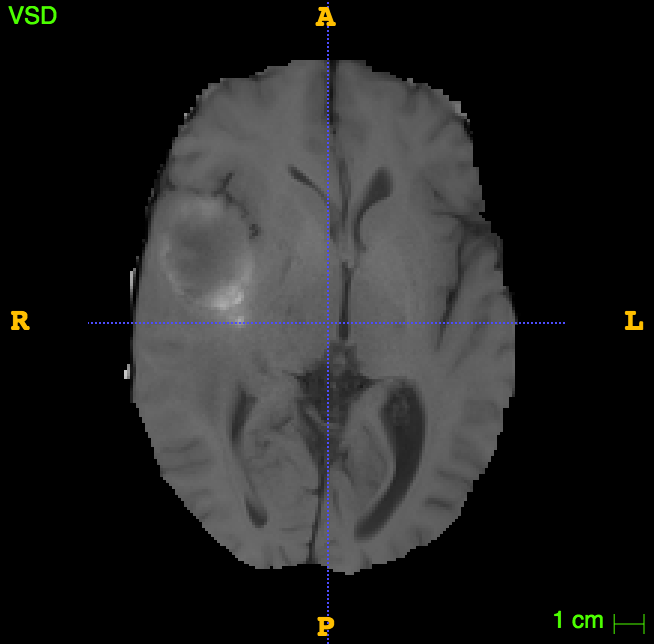
\includegraphics[scale=0.15]{T1_example}
	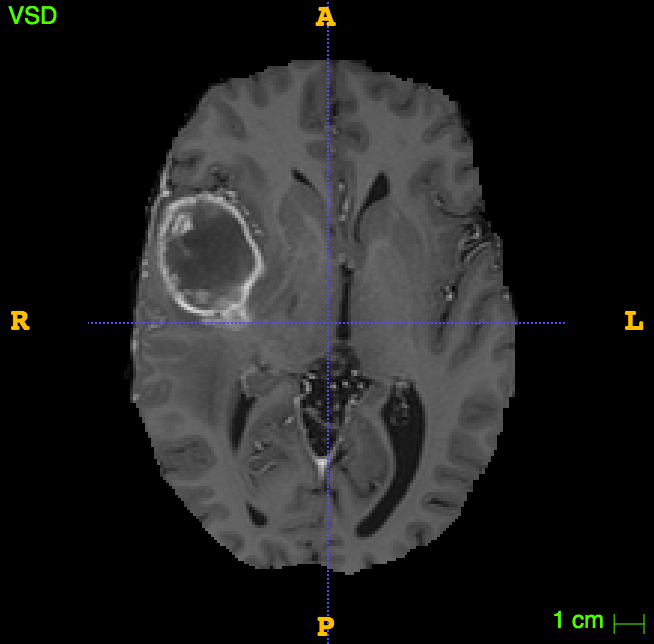
\includegraphics[scale=0.15]{T1c_example}
	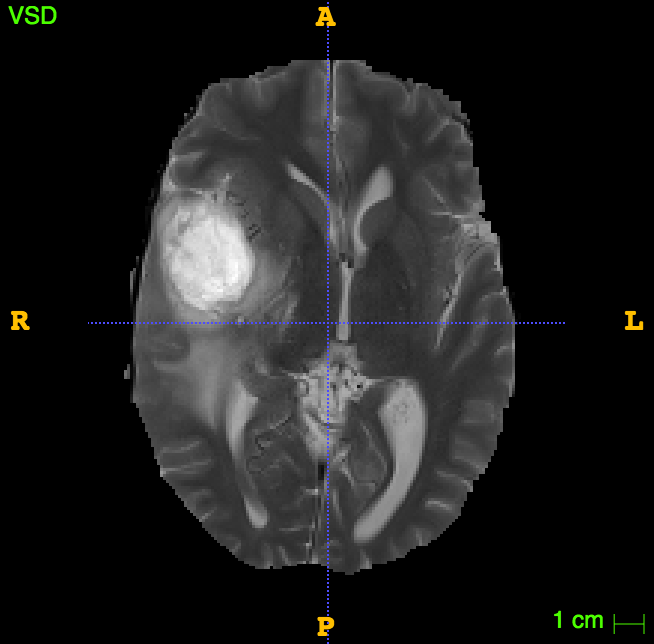
\includegraphics[scale=0.15]{T2_example}			
	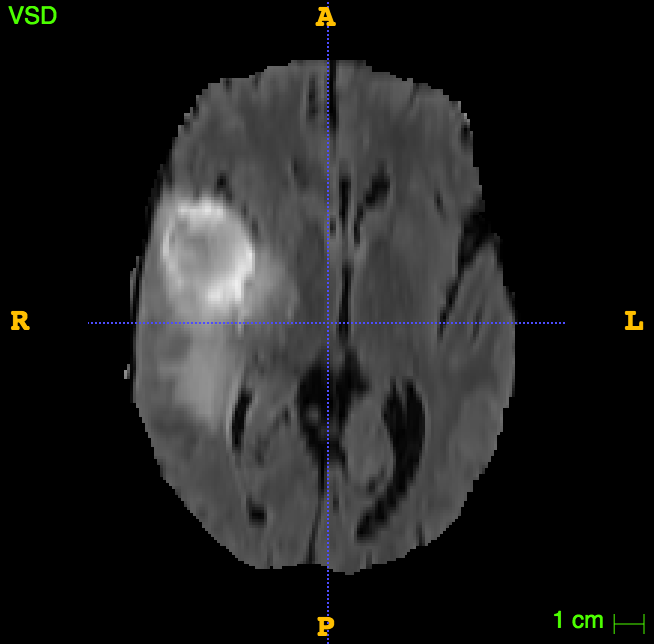
\includegraphics[scale=0.15]{Flair_example}
	\caption[Example slices in the axial plane for the 4 different scan modalities]{Example slices in the axial plane for the 4 different scan modalities. From left to right the modalities are T1, T1c, T2 and Flair. The scan is from patient 1, slice $z=89$. The four modalities have some obvious differences which the convolutional neural network might be able to utilise to discriminate between tumour and non-tumour regions.}
	\label{fig:mri_scans}
\end{figure}

To homogenise the data across the different scans, each patient's image volumes are co-registered to the T1c MRI scan, which has the highest spatial resolution in most cases. Then, all images are resampled to 1mm isotropic resolution in a standardised axial orientation with linear interpolation. Finally, all images are skull stripped to guarantee the anonymity of the patients.

The training dataset has been manually segmented by 4 different human experts into the 5 classes described in the introduction. These segmentations are then merged together to provide a single ground truth segmentation. As an example of what such a segmentation looks like I have included figure \ref{fig:expert_segmentations} which shows different slices of a T1 MRI scan annotated with the ground truth.

\begin{figure}
	\centering
	\includegraphics[scale=0.1]{expert_segmentation_49}
	\includegraphics[scale=0.1]{expert_segmentation_59}
	\includegraphics[scale=0.1]{expert_segmentation_69}
	\includegraphics[scale=0.1]{expert_segmentation_79}
	\includegraphics[scale=0.1]{expert_segmentation_89}
	\includegraphics[scale=0.1]{expert_segmentation_99}
	\includegraphics[scale=0.1]{expert_segmentation_109}
	\includegraphics[scale=0.1]{expert_segmentation_119}
	\includegraphics[scale=0.1]{expert_segmentation_129}
	\caption[Slices of a T1 MRI scan annotated with the expert labelling.]{Axial plane slices of a T1 MRI scan annotated by the expert labelling. The slices were taken from patient 1, using $z \in \{49, 59, 69, 79, 89, 99, 109, 119, 129\}$. The enhancing tumour region is in yellow, the non-enhancing tumour in blue, the edema in green and the necrotic core in red, corresponding to classes 4, 3, 2 and 1 respectively.}
	\label{fig:expert_segmentations}
\end{figure}



\subsection{High grade gliomas}
For this project I have decided to focus only on the high-grade glioma cases. I made this choice for the following reasons:
\begin{enumerate}
	\item To keep the scope of the project within that of a Part II project. Pereira et al.\ propose a different model for the low-grade glioma case which I would have had to replicate as well, possibly doubling the amount of work needed during the training phase.
	\item Secondly, the results of most research papers in this area are commonly reported in terms of high-grade glioma cases as it is considered to be harder than the low-grade cases. 
	\item Lastly, the challenge dataset, which consists only of high-grade patients allowed me to compare easily the results of my models with those of other researchers. Accordingly, I only use the 20 high-grade glioma cases of the training dataset to train the convolutional neural networks.
\end{enumerate}

\chapter{Implementation}
This chapter is divided into two parts, the first describing the implementation for the training of the model and the second describing how the trained model is used to segment MRI scans.

\section{Training the model}
\subsection{Scan normalisations}
\label{section:scan_normalisations}
The first step is to read in the scans, which is done using the SimpleITK library that has inbuilt support for the MetaImage medical (`.mha') format in which the images are made available. For each patient, the 4 scans (T1, T1c, T2, Flair) are read in as numpy arrays and stacked along a new dimension, resulting in a 4-dimensional array for each patient of shape $(z_{\text{size}} \times y_{\text{size}} \times x_{\text{size}} \times 4)$.
 
As explained in the previous chapter the data consists of 20 different patients, each consisting of 4 different MRI scans, taken with different modalities. Unfortunately, the size of the different scans varies from patient to patient. Table \ref{table:scan_sizes} shows how the sizes are distributed among patients. Because of this, the data for the patients cannot be aggregated into a single 5-dimensional numpy array. Instead, I aggregate those arrays into a single python list containing all the training data.

\begin{table}[h]
\centering	
\label{table:scan_sizes}
\begin{tabular}{ c c } 
\textbf{Size} & \textbf{Number of scans}\\
 \hline
 $\ 176 \times 216 \times 160$ & 8 \\ 
 $\ 176 \times 216 \times 176$ & 6 \\ 
 $\ 230 \times 230 \times 162$ & 2 \\ 
 $\ 176 \times 236 \times 216$ & 1 \\ 
 $\ 165 \times 230 \times 230$ & 1 \\ 
 $\ 240 \times 240 \times 168$ & 1 \\ 
 $\ 220 \times 220 \times 168$ & 1 \\ 

\end{tabular}
\caption{Scan sizes in voxels for the 20 different patients, dimensions are ordered as $(z \times y \times z)$}
\end{table}

The model proposed by Pereira et al. \cite{pereira} uses the Nyul normalisation \cite{nyul}. This normalisation requires human input, preferably from a domain expert, and I was therefore not able to use that normalisation method. The paper also proposes a second normalisation method, done by first winsorising the scans and then applying the N4 normalisation. This method performed slightly worse but had the advantage of being fully automated, which is why I chose to use this method for the normalisation stage.

\subsubsection{Winsorising}
The first normalisation that is applied to entire scans is called `winsorising'. The aim is to limit the values of extremes, in order to reduce the effect that outliers may have. This is also known as `clipping' in digital signal processing. I used a 98\% winsorisation, meaning that the data values below the 1\textsuperscript{st} percentile are set to the value of the 1\textsuperscript{st} percentile and the value above the 99\textsuperscript{th} percentile are set to the value of the 99\textsuperscript{th} percentile. Note that this process is different from trimming as the values are not discarded but just clipped.

\subsubsection{N4 Bias field correction}
The second normalisation applied to scans is the N4 bias field correction \cite{n4itk}. MRI scanner can create a bias in which the intensity of the same tissue varies across the produced scan, making it hard for automated segmentation algorithms to recognise that it is in fact the same tissue. N4 is a variant of the popular nonparametric nonuniform intensity normalisation N3 which aims at eliminating this bias introduced by MRI scanners. 

As this correction is rather complicated and not the main point of my project, I will not go into more details here. However, for completeness, table \ref{table:n4_params} lists the parameters I used to perform the normalisation. I first used the default parameters and later contacted Pereira who kindly agreed to share the parameters he used in his published method, which are reported here. I used the implementation provided by the `Nipype'\footnote{\url{http://nipype.readthedocs.io/en/latest/}} and the `Advanced Normalization Tools'\footnote{\url{http://stnava.github.io/ANTs/}}.

\begin{table}[h]
\centering	
\begin{tabular}{ c c } 
\textbf{Parameter} & \textbf{Value} \\
 \hline
 n\_iterations & [20,20,20,10] \\ 
 dimension & 3 \\
 bspline\_fitting\_distance & 200 \\
 shrink\_factor & 2\\
 convergence\_threshold & 0
\end{tabular}
\caption{Parameters used to perform the N4ITK correction.}
\label{table:n4_params}
\end{table}

Figure \ref{fig:n4itk_example} shows the effects that winsorising and then applying the N4 bias field correction has on scans for each of the four modalities T1, T1c, T2 and Flair.
\begin{figure}
	\centering
	\label{fig:n4itk_example}
	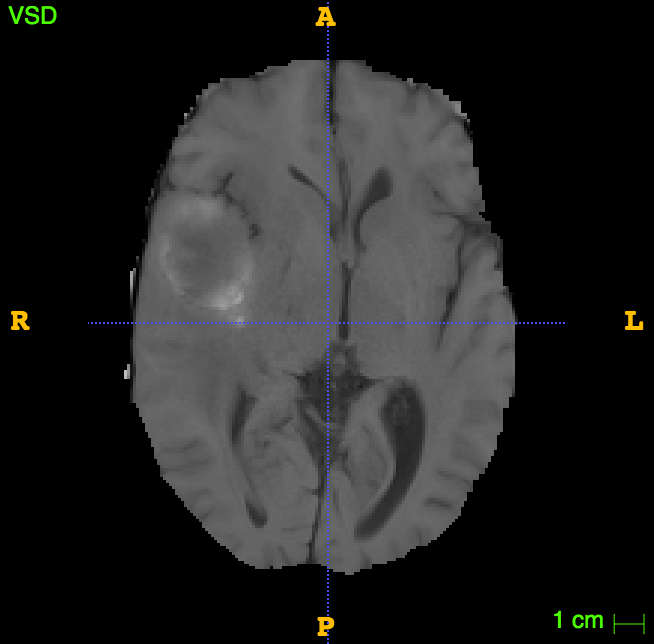
\includegraphics[width=0.3\textwidth]{t1_no_norm_example}
	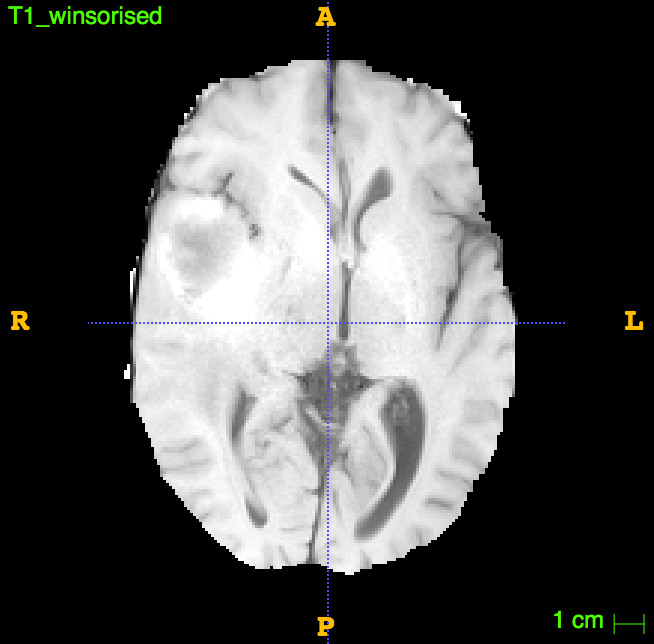
\includegraphics[width=0.3\textwidth]{t1_winsorized_example}
	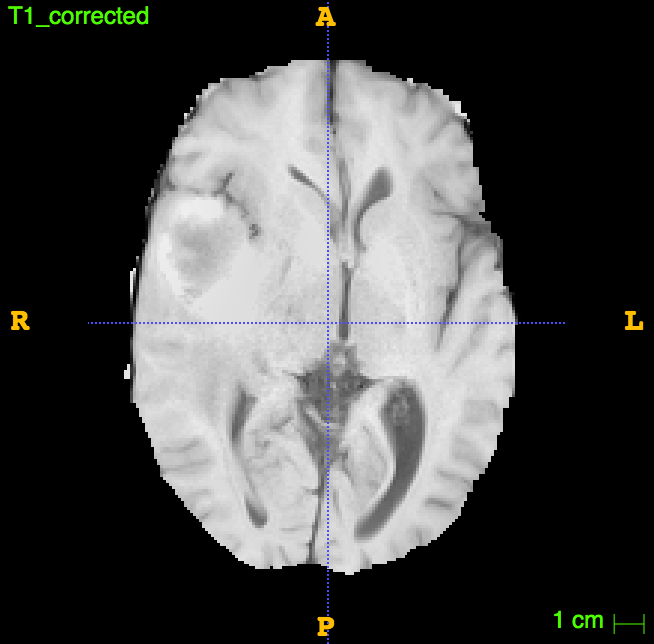
\includegraphics[width=0.3\textwidth]{t1_n4itk_example} \\
	\vspace{0.5cm}
	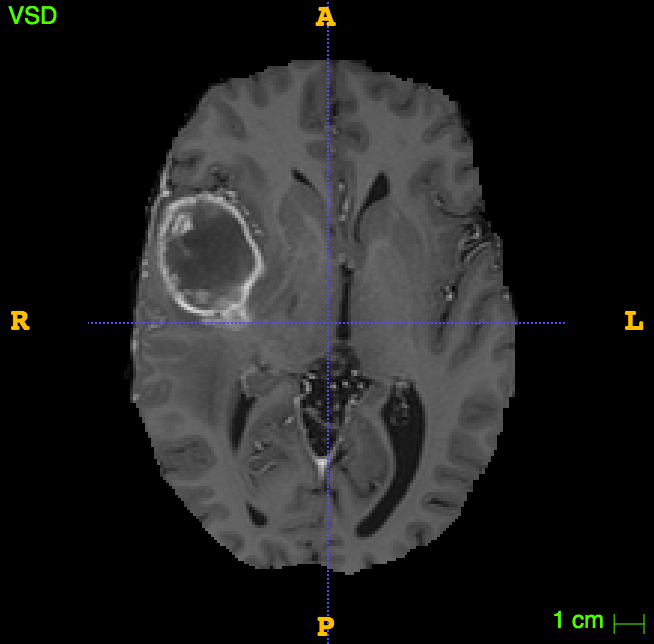
\includegraphics[width=0.3\textwidth]{t1c_no_norm_example}
	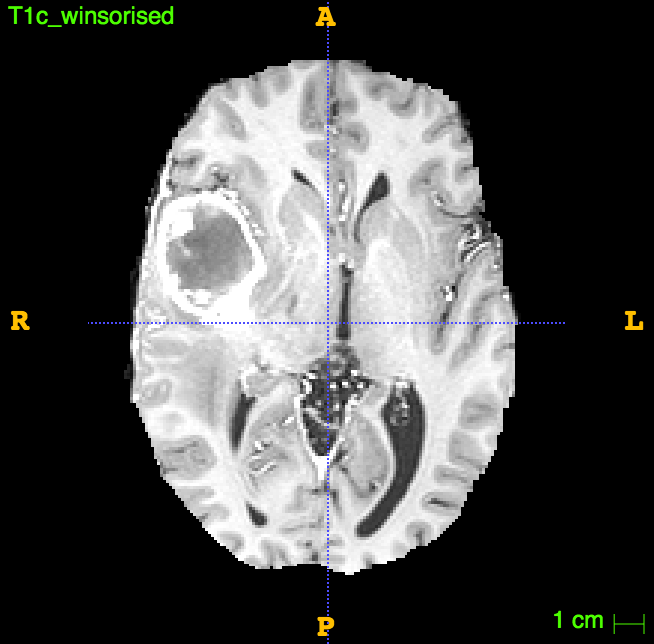
\includegraphics[width=0.3\textwidth]{t1c_winsorized_example}
	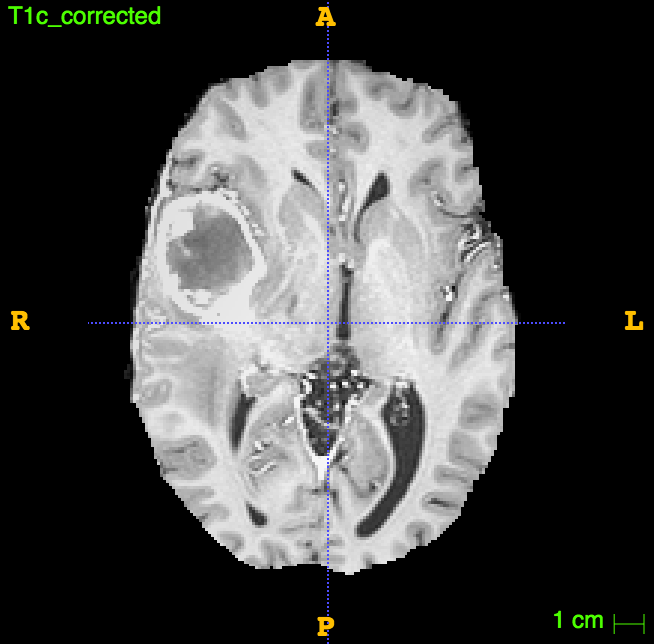
\includegraphics[width=0.3\textwidth]{t1c_n4itk_example} \\
	\vspace{0.5cm}
	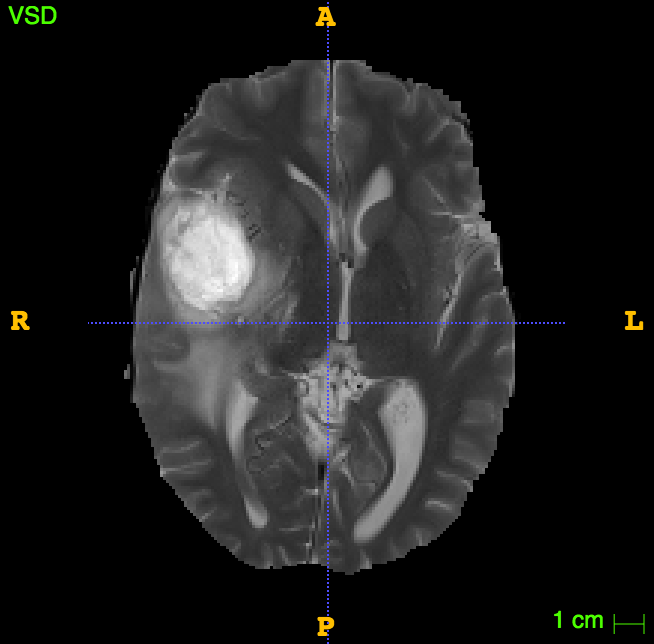
\includegraphics[width=0.3\textwidth]{t2_no_norm_example}
	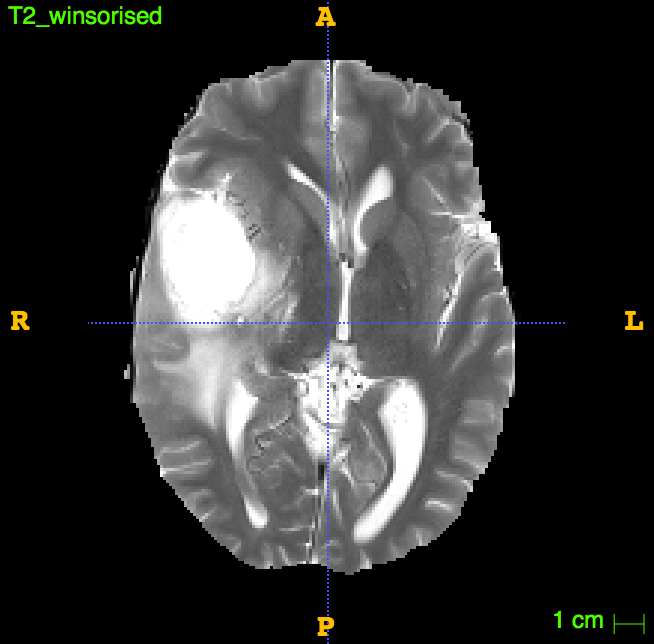
\includegraphics[width=0.3\textwidth]{t2_winsorized_example}
	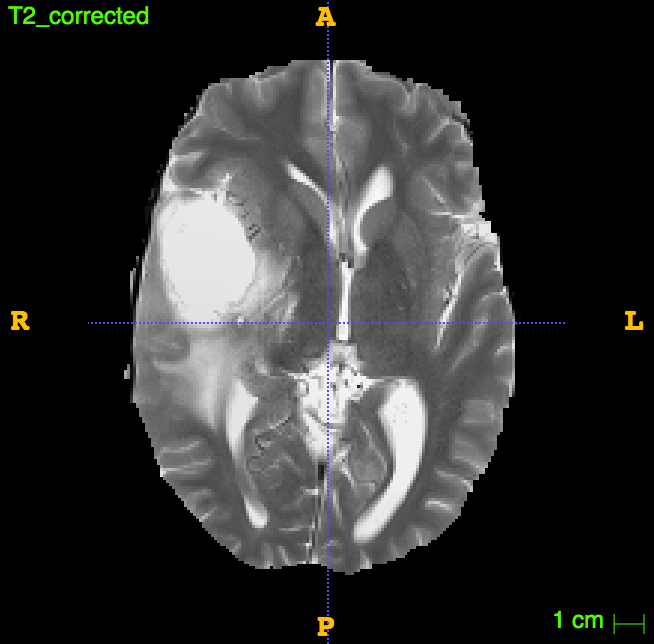
\includegraphics[width=0.3\textwidth]{t2_n4itk_example} \\
	\vspace{0.5cm}
	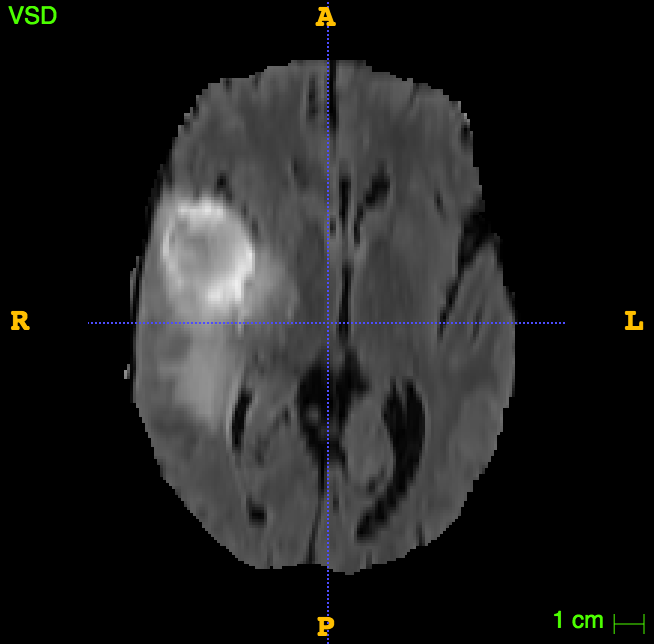
\includegraphics[width=0.3\textwidth]{flair_no_norm_example}
	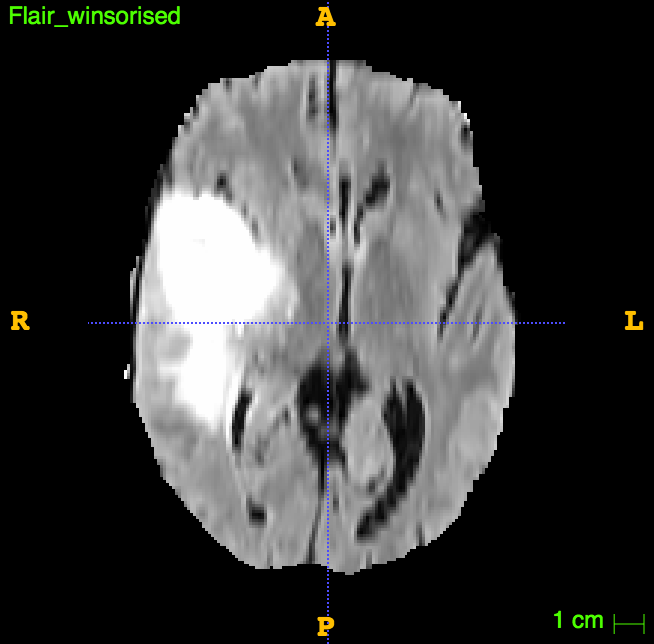
\includegraphics[width=0.3\textwidth]{flair_winsorized_example}
	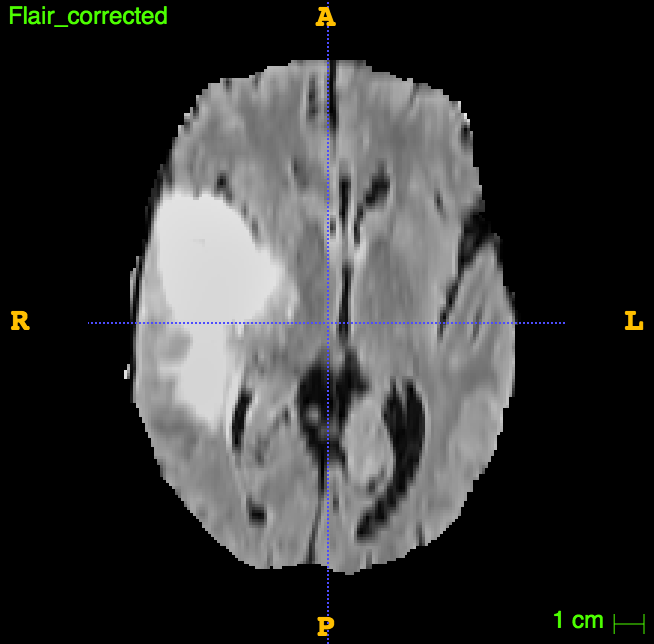
\includegraphics[width=0.3\textwidth]{flair_n4itk_example}
	\caption{Example of the effects of winsorising and applying the N4ITK correction applied to scans for each of the four modalities. The first image in each row is the original scan, the middle image is obtained by winsorizing the original image and the last image is obtained by applying the N4ITK correction to the winsorised scan. From top to bottom, slice $z=89$ is shown for patient 1 for the T1, T1c, T2 and Flair scans.}
\end{figure}

\subsubsection{Mean and Variance standardisation}
The last step is to standardise the mean and variance for each scan along each slice. This is done by first subtracting the mean value of the voxels in the slice and then dividing by the standard deviation of those values. 
\begin{equation}
	x' = \frac{x - \mu}{\sigma}
\end{equation}
As $\mathbb{E}[aX] = a \mathbb{E}[X]$ and $\textrm{Var} [cX] = c^2 \textrm{Var} [X]$ one can show that after this transformation the new mean will be 0 and the standard deviation will be 1. Also note that as the true mean and standard deviation are not known, the sample mean and sample standard deviation must be used. 

I use numpy's \texttt{mean} and \texttt{std} functions and the fact that basic operations on numpy arrays are done element-wise to implement this normalisation.

\subsection{Patch extraction}
\label{section:patch_extraction}
Each input to the convolutional neural network is a three-dimensional array, of shape $\textsf{height} \times \textsf{width} \times 4$, since it consists of a two-dimensional patch of $\textsf{width} \times \textsf{height}$ voxels for each one of the 4 scan modalities. The two-dimensional patches are taken along the x--y axis, also called the axial plane in anatomy. Figure \ref{fig:patch_extraction} gives a diagramitic overview of the transformation for the simplified case with a single modality, meaning that the image array is three-dimensional and the resulting patch is two-dimensional, instead of four and three-dimensional respectively.
\begin{figure}
	\centering
	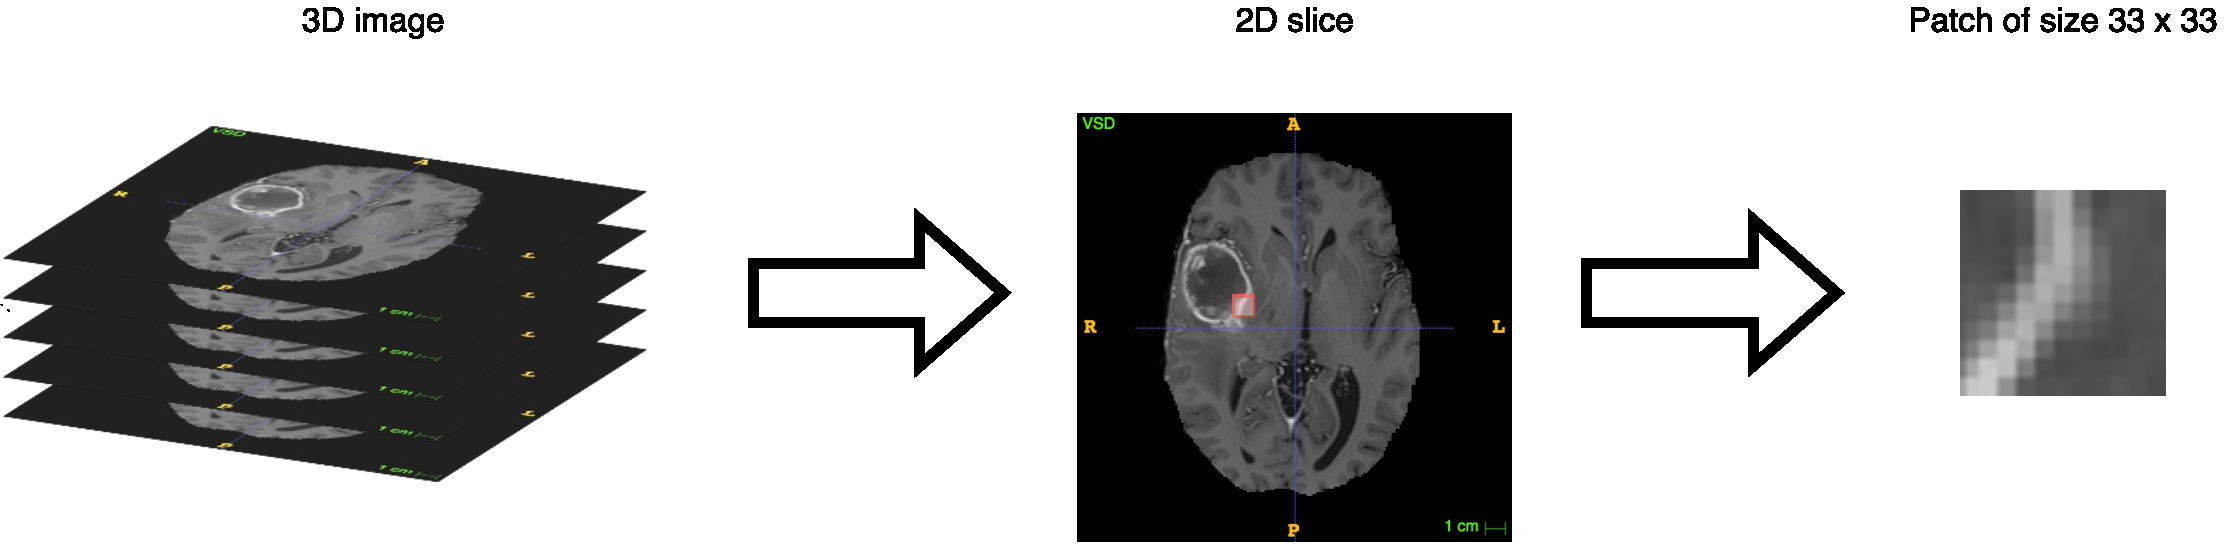
\includegraphics[width=\textwidth]{patch_extraction}
	\caption[Patch extraction process for a three dimensional array.]{Patch extraction process for a three dimensional array. The actual image array is four dimensional, the 4th dimension being the different modalities. Here $\textsf{width}=\textsf{height}=33$ and therefore corresponds to the patch size proposed by pereira et al.}
	\label{fig:patch_extraction}
\end{figure}

There are two issues that need to be resolved before extracting the patches:
\begin{enumerate}
	\item The training data has to be balanced, meaning that the same number of examples for each class should be included in the training data. This is to ensure that the convolutional model is able to generalise well. However, the BraTS dataset is extremely unbalanced with over 98\% of the voxels belonging to class 0, as shown in table \ref{table:class_frequencies}. Therefore, simply randomly picking patches from the dataset does not work. Also note that a fixed balanced dataset would limit the maximum number of patches we can extract to 5 times the number of voxels in the least represented class. This is the non-enhancing tumour class (class 3) with 184,436 labeled voxels, hence a maximum of 922,130 patches. To increase the number of different patches the network sees during training for the overrepresented classes while keeping the data balanced, I randomly resample at each epoch the same number of patches for each class from all possible patches for that class.
		\begin{table}
			\centering	
			\begin{tabular}{c c S[table-format=9.0] S[table-format=2.2]}
			\textbf{Class} & \textbf{Tissue type} & \textbf{Number of labeled voxels} & \textbf{frequency}\\
			 \hline
			0 & Non tumour 				& 138958832 	& 98.23 \% \\ 
			1 & Necrosis 				& 282936 	& 0.20 \% \\ 
			2 & Edema					& 1466271 	& 1.36 \% \\ 
			3 & Non-enhancing tumour 	& 184436 	& 0.13 \% \\ 
			4 & Enhancing tumour		& 560777 	& 0.34 \% \\
			
			\end{tabular}
			\caption{Class frequencies in the BraTS2013 HG dataset. The normal tissue (class 0) is highly overrepresented, which leads to issues when training the convolutional neural network. We therefore have to balance the dataset when extracting the patches.}
			\label{table:class_frequencies}
		\end{table}
	\item It is not possible to extract an entire patch around the voxels too close to the edge of the scan. To solve this issue there are two options: I could either ignore the patch entirely or pad the scan such that each labelled voxel is surrounded by enough voxels. Only the first option is considered as it helps with the balanced classes issue as most of the voxels close to an edge are from class 0. Furthermore, as the brains are centred within the MRI scans, voxels close to and edge are surrounded only by voxels of value 0, making the patch identical to many other patches close to an edge. Table \ref{table:valid_class_frequencies} shows the distribution of classes for ``valid'' voxels, .i.e those at least more than half the patch length away from the x or y edges for the Pereira model with $\textsf{width}=\textsf{height}=33$. Indeed, most ignored voxels come from class 0.

		\begin{table}[h]
		\centering	
		\begin{tabular}{c c S[table-format=9.0] S[table-format=2.2] S[table-format=8.0]}
		\textbf{Class} & \textbf{Tissue type} & \textbf{Labelled voxels} & \textbf{Frequency} & \textbf{Ignored voxels}\\
		 \hline
		0 & Non tumour 				& 94773429 	& 97.45 \% & 44185403 \\ 
		1 & Necrosis 				& 281831 	& 0.29 \% & 1105\\ 
		2 & Edema					& 1453205 	& 1.49 \% & 13066\\ 
		3 & Non-enhancing tumour 	& 183396 	& 0.19 \% & 1040\\ 
		4 & Enhancing tumour		& 558320 	& 0.57 \% & 2457\\
		\end{tabular}
		\caption{Class frequencies in the BraTS2013 HG dataset for valid voxels only, that is, those voxels it is possible to extract a patch of size $33 \times 33$ around. As most of the ignored voxels are in class 0, we can safely ignore them.}
		\label{table:valid_class_frequencies}
		\end{table}
\end{enumerate}

In his email, Pereira mentioned that he used two further heuristics for extracting patches from class 0 that were not mentioned in his paper, which I also implemented:
\begin{enumerate}
	\item Half of the patches for class 0 are selected close to the tumour, where close means that the central voxel is within the bounding box of the diseases tissue. This helps the network to learn how to draw the boundaries between class 0 and the other classes.
	\item The other half of the training patches for class 0 are spaced apart with a distance of at least 3 voxels in the z,y and x directions. This spreads the input data to the entire scan.
\end{enumerate}


\subsubsection{Algorithm}
To make the resampling of the patches at each epoch more efficiently, I first create a list (\texttt{valid\_positions}) containing for each class the positions of the valid patches (really the position of the central voxel) for that class. Note that at this point it would be unfeasible to store all possible patches, as it would require to store over a 100 billion 32 bit floats for class 0 alone, or over 400 GB. To get the indices of the valid voxels, I used numpy's argwhere function on the ground truth arrays. The argwhere function takes in an array and a predicate and returns the indices of those elements in the array satisfying the predicate. I use equality checking between the voxel label and the class number. This is done for every patient and returns an array consisting of the $(z, y, x)$ coordinates of valid patches for every patient. Since the patient number must also be included in the indices, I prepend the patient number along the first axis, resulting for each patient in an array consisting of the $(\text{patient}, z, y, x)$ coordinates and aggregate the results for each patient into a single list. The second step consists of removing those voxels that are too close to an x-axis or y-axis edge. Only indices $(\text{patient}, z, y, x)$ where the x and y values are  within the allowed ranges defined by half the size of the patch: $[\lfloor \frac{\textsf{width}}{2} \rfloor, \textsf{width}_{\text{scan}} - \lceil \frac{\textsf{width}}{2} \rceil]$ and respectively for the height are kept. Again this can be done using numpy and filtering based on column values. Algorithm \ref{alg:patch_extraction} summarises the steps taken during the patch extraction. 

\begin{algorithm}
\caption{Patch extraction}\label{alg:patch_extraction}
\begin{algorithmic}[1]
\For{$\text{class } k \text{ in } [0,1,2,3,4]$}
	\State valid\_positions[$k$] $\gets$ []
	\For{\textbf{each} index \textbf{in} len(labels)}
		\State label $\gets$ labels[index] 
		\State possible\_indices $\gets$ \textit{numpy}.argwhere(label == $k$)
		\State patient\_indices $\gets$ \textit{numpy}.full(\textit{len}(possible\_indices), index)
		\State possible\_indices $\gets$ \textit{numpy}.append(patient\_indices, possible\_indices, axis = 1)
		\State
		\State possible\_indices $\gets$ possible\_indices[$\text{possible\_indices}[:,2] \ge \lfloor \frac{\textsf{height}}{2} \rfloor$]
		\State possible\_indices $\gets$ possible\_indices[$\text{possible\_indices}[:,2] \leq \text{height}_{\text{label}} - \lceil \frac{\textsf{height}}{2} \rceil$]
		\State possible\_indices $\gets$ possible\_indices[$\text{possible\_indices}[:,3] \ge \lfloor \frac{\textsf{width}}{2} \rfloor$]
		\State possible\_indices $\gets$ possible\_indices[$\text{possible\_indices}[:,3]  \leq  \text{width}_{\text{label}} - \lceil \frac{\textsf{width}}{2} \rceil$]
		\State
		\State valid\_indices[$k$] $\gets$ possible\_indices
	\EndFor
\EndFor
\end{algorithmic}
\end{algorithm}

At the beginning of each training epoch, I then randomly choose the same number of positions for each class from \texttt{valid\_positions} using numpy's \texttt{random.choice} function. For each position I extract the corresponding patch and label which are returned as training data.

\subsection{Data augmentation}
To increase the amount of data available, some data augmentation techniques can be used. In typical applications of convolutional neural networks for image processing and computer vision tasks, translation and rotations are be used. Since the data consists entirely of two-dimensional patches, translation is useless as it would just result in a different patch, with a possibly different label. However, using rotations of the patches might give some performance improvements. Pereira et al. propose the following variants in \cite{pereira}:
\begin{enumerate}
	\item No rotations
	\item Rotations of 90, 180 and 270 degrees.
	\item Uniformly sample three rotations from an array of equally spaced angles. The angle step proposed is $\frac{1}{16} \times 90^{\circ} = 6^{\circ}$
\end{enumerate}
Pereira et al. reported that using rotations of multiples of 90 degrees performed the best, which is why I decided to implement it. I perform the rotations with a custom Keras `data generator'. Such a data generator receives as an input a batch of data and returns another batch of data. Here, the generator just randomly rotates each training patch in the batch using the numpy \texttt{rot90} function which rotates arrays by steps of 90 degrees.

\subsection{Training: Pereira model}

\subsubsection{Architecture}

The model proposed by Pereira et al. \cite{pereira} consists of 11 layers, shown in figure \ref{fig:pereira_model}. The first three layers are convolutional layers with filter size $3 \times 3$, stride $1 \times 1$ and width 64. Using three layers of size $3 \times 3$ consecutively effectively has a receptive field of size $7 \times 7$, but has fewer parameters then a single $7 \times 7$ convolutional layer would have, reducing the overall number of parameters and therefore making the network less prone to overfitting \cite{very_deep_conv_nets}. The next layer is a max pooling layer of size $3 \times 3$ and stride $2 \times 2$. This is an unusual design choice for convolutional networks as the size is typically smaller than the stride. Pereira et al. motivate this choice because although pooling can be positive to eliminate unwanted details and achieve invariance, it can also eliminate some of the important details. By keeping the size of the layer larger than the stride, the pooling will overlap which will allow the network to keep more information about location. Next, three more consecutive convolutional layers are applied, this time doubling the width to 128 filters. Again a max pooling layer with the same hyper-parameters as the previous one is applied, before adding three fully-connected layers of size 256, 256 and 5 respectively. Table \ref{table:pereira_weights} shows the model architecture in more details including the number of weights in each layer. 

\begin{figure}
	\centering
	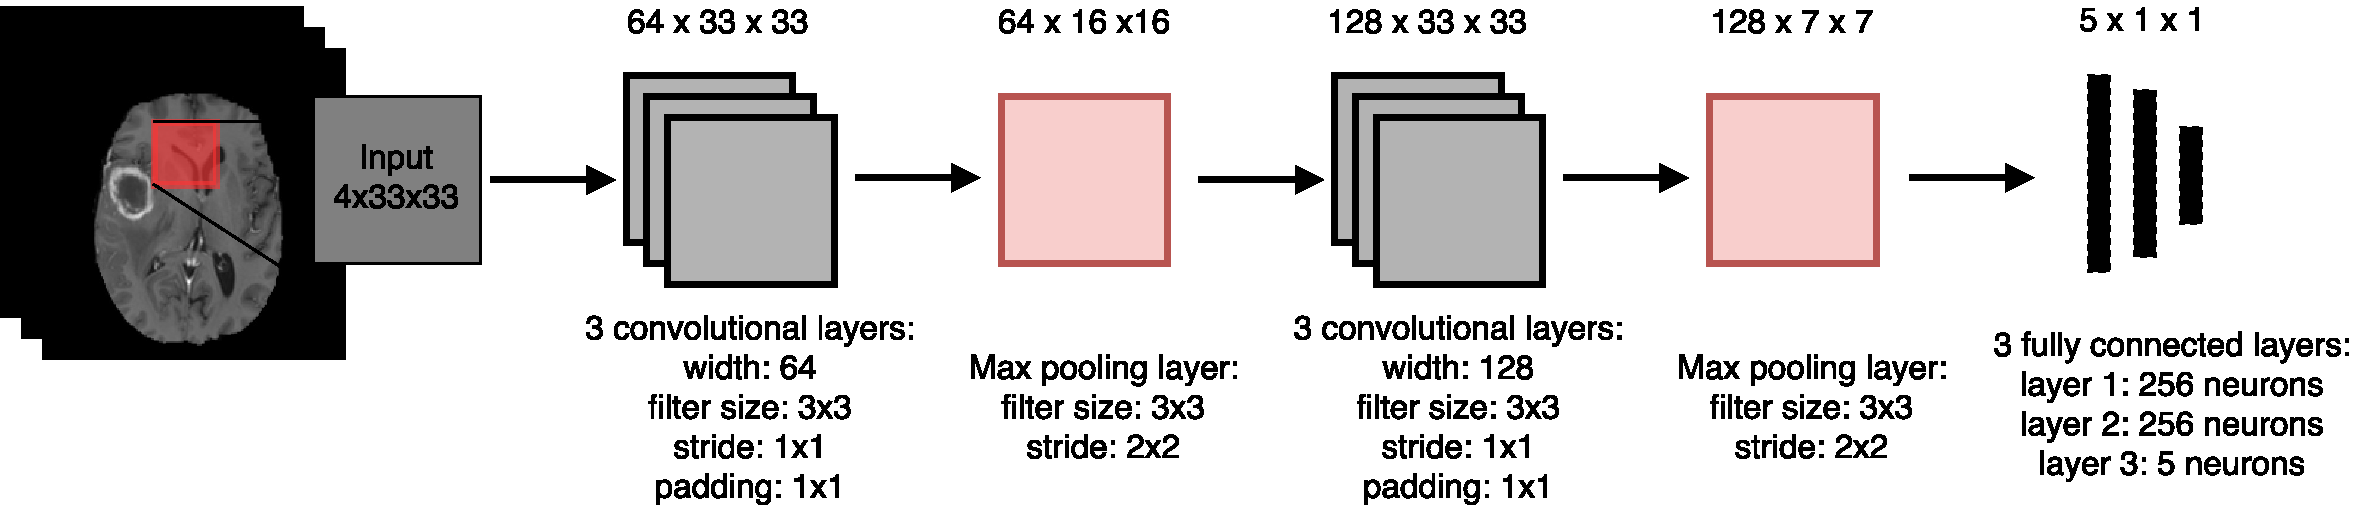
\includegraphics[width=\textwidth]{pereira_model}
	\caption{Convolutional network architecture proposed by Pereire et al.}
	\label{fig:pereira_model}
\end{figure}

\begin{table}
\centering	
\label{table:pereira_weights}
\begin{tabular}{ c c S[table-format=7.0] } 
\textbf{Layer type} & \textbf{Output shape} & \textbf{\# Parameters} \\
 \hline
 Conv 		& $\ 64 	\times 33 	\times 33$ 	& 2368 \\ 
 Conv 		& $\ 64 	\times 33 	\times 33$ 	& 36928 \\ 
 Conv 		& $\ 64 	\times 33 	\times 33$	& 36928 \\ 
Max-Pool 	& $\ 64 	\times 16 	\times 16$ 	& 0\\
 Conv 		& $128 		 \times 16 	\times 16$	& 73856 \\ 
 Conv 		& $128 		\times 16 	\times 16$ 	& 147584 \\ 
 Conv 		& $128 		\times 16 	\times 16$ 	& 147584 \\ 
Max-Pool 	& $128 		\times\ 7 	\times\ 7$	& 0\\
FC			& $256 		\times\ 1 	\times\ 1$	& 1605888\\
FC			& $256 		\times\ 1 	\times\ 1$	& 65792\\
FC			& $\quad 5 	\times\ 1 	\times\ 1$ 	& 1285\\
\hhline{~~=}
\rule{0pt}{3ex}    
&& 2118213\\
\end{tabular}
\caption[Summary of the architecture proposed by Pereira, including the number of parameters in each layer.]{Summary of the architecture proposed by Pereira, including the number of parameters in each layer. The network has a total of 2,118,213 trainable parameters.}
\end{table}


The weights in the convolutional layers are initiliased using Xavier normal initialisation \cite{xavier_init}. The biases are initialised to the constant value 0.1, except for the last layer.

The activation function used throughout the network is the leaky rectifier, with  $\alpha = 0.333$.

Of the three techniques presented in the preparation chapter to avoid overfitting, only Dropout \cite{dropout} is used in the fully-connected layers, with probability $p=0.1$ of removing a node from the network.

\subsubsection{Implementation of the architecture in Keras}
The network proposed by Pereira et al. is sequential, meaning that the layers are stacked linearly. Using the keras \texttt{Sequential} model is therefore the simplest way to implement it. The \texttt{Sequential} model makes it possible to create networks by adding layers to it sequentially. The three types of layers used in the network have available Keras implementations, and therefore building the network itself was relatively straightforward. First, an instance a of a sequential model is instanciated:
\begin{lstlisting}[language=Python]
	model = Sequential()
\end{lstlisting}
Then, layers can be added by calling the \texttt{add} function on the model. For example to add a convolutional layer, we first create an instance of the \texttt{Convolution2D} class and then add it to the model:
\begin{lstlisting}[language=Python]
	conv = Convolution2D(nb_filters, width, height, border_mode='same', init='glorot_normal')
	model.add(conv)
\end{lstlisting}
The library makes it easy for the user to specify how the weights should be initialised by setting the \texttt{init} argument. The \texttt{border\_mode} argument determines the size of the padding that is added to input before applying the convolutional layer. In our case the output of the layer should have the same size as the input, which is specified by setting the argument to `same'. Max pooling layers and fully-connected layers can be added similarly using instances of \texttt{MaxPooling2D} and \texttt{Dense} classes respectively.

Activation functions are added in the same way as layers. Hence, to add a leaky rectifier, also called LReLU, we add an instance of the \texttt{LeakyReLU} class to the model:
\begin{lstlisting}[language=Python]
	alpha = 0.333
	LReLU = LeakyReLU(alpha)
	model.add(LReLU)
\end{lstlisting}
Adding Dropout is again done similarly:
\begin{lstlisting}[language=Python]
	p = 0.1
	model.add(Dropout(p))
\end{lstlisting}

Finally, before training the model, we need to specify which loss function and which algorithm should be used to respectively specify and minimise the loss function. In Keras this is called `compiling' the model:
\begin{lstlisting}[language=Python]
	sgd = SGD(lr=3e-5, decay=0.0, momentum=0.9, nesterov=True)
	model.compile(optimizer=sgd, loss='categorical_crossentropy', metrics=['accuracy']
\end{lstlisting}

\subsubsection{Training}
The paper specifies that the model was trained over 20 epochs, each training the network on 450,000 patches. As no more details are specified, I use 90,000 patches per class selected at random as explained in section \ref{section:patch_extraction}. The optimisation algorithm used is a standard stochastic gradient descent algorithm with Nesterov momentum, with constant momentum $\mu = 0.9$. The learning rate is linearly decreased from $3 \times 10^{-5}$ to $3 \times 10^{-7}$. As Keras does only have an implementation for exponential learning rate decay, I use algoritm \ref{alg:linear_decay} to manually specify the learning rate at each epoch.

\begin{algorithm}
\caption{Model training with linear learning rate decay}
\label{alg:linear_decay}
\begin{algorithmic}[1]
\For{$i \text{ from } 0 \text{ to } \text{nb\_epochs}-1$} 
	\State $\text{learning\_rate} \gets \text{start\_rate} + i \times \dfrac{\text{end\_rate} - \text{start\_rate} }{ \text{nb\_epochs} - 1 }$
	\State train\_model(nb\_epochs = 1, learning\_rate)
\EndFor
\end{algorithmic}
\end{algorithm}

At the end of each epoch the loss function is evaluated on the validation data and the accuracy (equation \ref{eq:accuracy}) is computed. The loss and accuracy are then reported to the standard output. Figure \ref{fig:training_output} shows part the output of training a network for a few epochs.
\begin{equation}
	\label{eq:accuracy}
		\text{accuracy} = 
	\frac{1}{m}\Big[\sum_{i=1}^m\mathbbm{1}[y^{(i)} = \argmax{k}P(y^{(i)}=k)]\Big]
\end{equation}
\begin{figure}
	\centering
	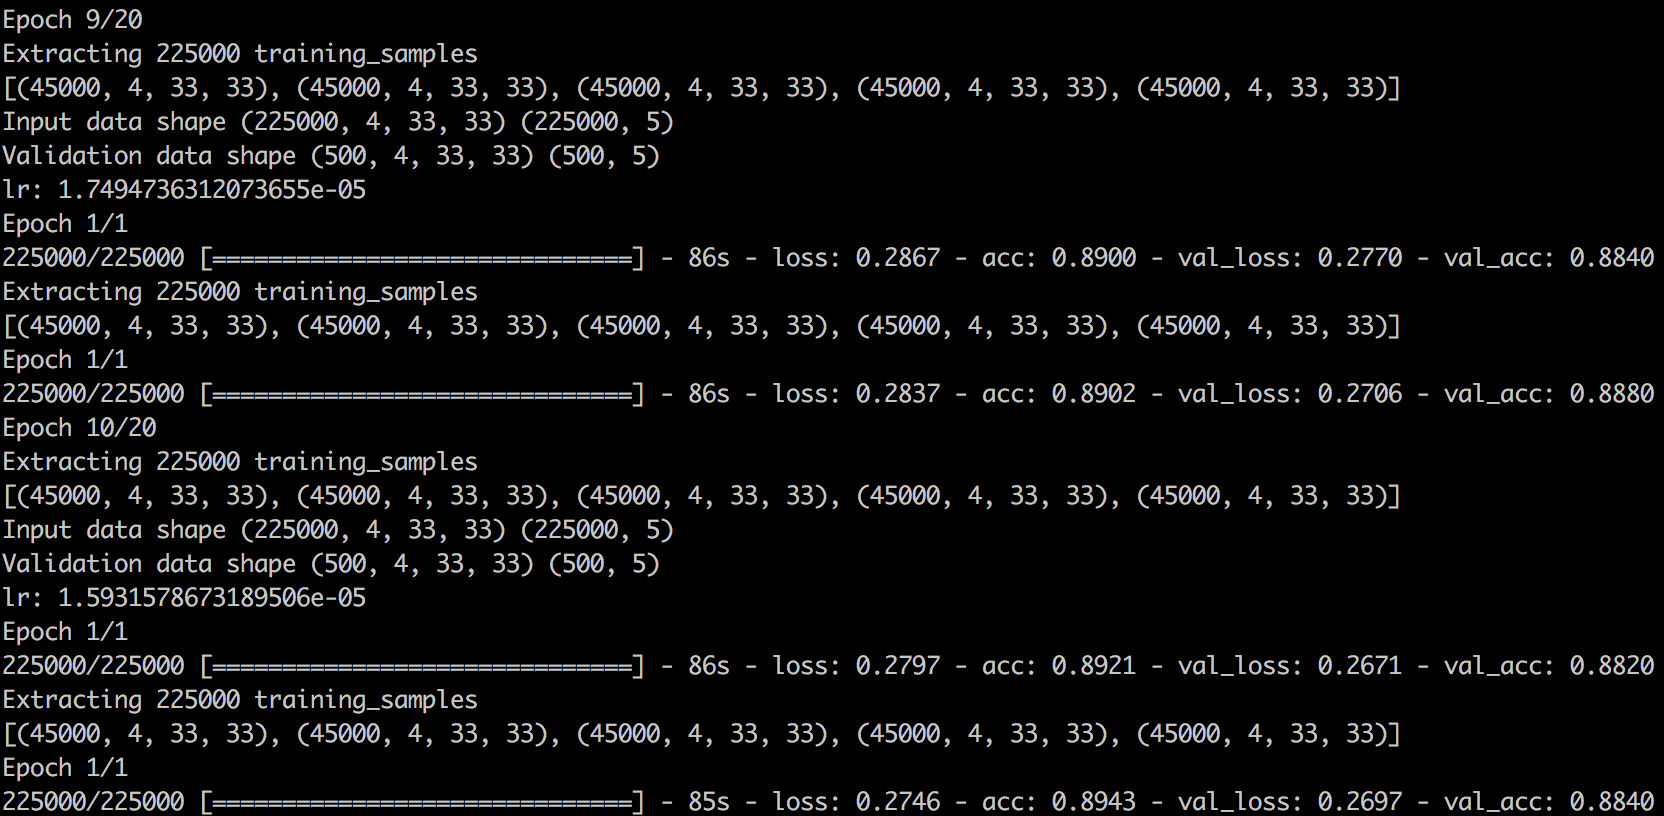
\includegraphics[width=\textwidth]{training_output}
	\caption[Part of the output of the training script]{Part of the of the training script. The output is shown for epochs 9 and 10. Both the validation loss and the validation accuracy are reported, as well as how long it took to train and validate for this epoch. Because all 450,000 patches cannot be held at once in memory, the epoch is divided into two training phases, each on 225,000 patches.}
	\label{fig:training_output}
\end{figure}

After training the model for 20 epochs, I save the model with its weights in a directory specified as an argument to the main python script, so that I can reload the model for the segmentation of MRI scans. 

In figure \ref{fig:pereira_validation_loss} the validation loss and validation accuracy are plotted for the 20 epochs. Both seem to converge over this period. The validation accuracy is higher than the training accuracy because of Dropout: during validation no neurons are dropped, meaning that the entire network is used which is therefore able to classify the data more accurately.

\begin{figure}
	\centering
	\setlength\figureheight{10cm}
	\setlength\figurewidth{0.8\textwidth}
	% This file was created by matplotlib2tikz v0.6.6.
\begin{tikzpicture}

\definecolor{color0}{rgb}{0,0.75,0.75}

\begin{axis}[
xlabel={Training epoch},
xmin=1, xmax=20,
ymin=0.5, ymax=1.2,
axis on top,
width=\figurewidth,
height=\figureheight,
tick pos=both,
legend cell align={left},
legend entries={{training loss},{validation loss},{training accuracy},{validation accuracy}}
]
\addplot [blue]
table {%
1 1.13041391290877
2 0.861061694403754
3 0.767879048654768
4 0.718250204766591
5 0.687153879943424
6 0.657512406135135
7 0.638395594535404
8 0.619145059149
9 0.603178794184791
10 0.588090721172757
11 0.576668203987545
12 0.566907474208408
13 0.559151472159492
14 0.552124424449073
15 0.546010555464427
16 0.543806777116987
17 0.538134276373122
18 0.535040917841593
19 0.533549856452942
20 0.531543177839915
};
\addplot [green!50.0!black]
table {%
1 0.963762547492981
2 0.842494929790497
3 0.776172799110413
4 0.736501190185547
5 0.70885239648819
6 0.68199206829071
7 0.662558878898621
8 0.656801614761353
9 0.639917059421539
10 0.625560926914215
11 0.608640273094177
12 0.607184840679169
13 0.593906958580017
14 0.585756418228149
15 0.580585649013519
16 0.581344957828522
17 0.576201499462128
18 0.572517706394196
19 0.570800209522247
20 0.569466398239136
};
\addplot [red]
table {%
1 0.529084444442325
2 0.660106666662428
3 0.700079999995761
4 0.718871111111111
5 0.732142222222222
6 0.742719999997881
7 0.74996888888465
8 0.758364444448683
9 0.764888888888889
10 0.770831111111111
11 0.776053333335453
12 0.779055555559794
13 0.783113333335453
14 0.78538
15 0.788662222224341
16 0.788593333337572
17 0.791597777779897
18 0.792982222220103
19 0.793551111111111
20 0.794337777777778
};
\addplot [color0]
table {%
1 0.618400000572205
2 0.673599999904633
3 0.687200001239777
4 0.710399997711182
5 0.719199996948242
6 0.731599998474121
7 0.743199998855591
8 0.73800000333786
9 0.747599998474121
10 0.754399999141693
11 0.759200000762939
12 0.759600001811981
13 0.765999997615814
14 0.76360000038147
15 0.76840000295639
16 0.763600002288818
17 0.774400001049042
18 0.77040000295639
19 0.773200002193451
20 0.773600001811981
};
\end{axis}

\end{tikzpicture}
	\caption[Validation loss and accuracy during training for the model proposed by Pereira et al.]{Validation loss and accuracy during training for the model proposed by Pereira et al. Both seem to converge over this period.}
	\label{fig:pereira_validation_loss}
\end{figure}

\subsection{Training: My model}
\subsubsection{Architecture}
The design of the architecture for my model is based on the following points:
\begin{enumerate}
	\item I increase the size of the input patches, almost doubling it to $64 \times 64$. Using this bigger patch, the model should be able to incorporate more contextual information from voxels further away in the slice for the classification. Figure \ref{fig:bigger_patches} shows the difference in patch size.
		\begin{figure}
			\centering
			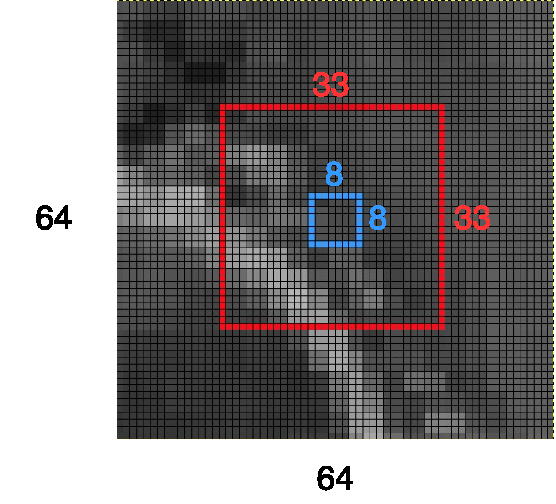
\includegraphics[width=0.4\textwidth]{bigger_patches}
			\caption[Example patch for my model compared to a patch for the model proposed by Pereira et al. \cite{pereira}]{Example patch for my model compared to a patch for the model proposed by Pereira et al. \cite{pereira}. The patch for the Pereira model is drawn in red.}
			\label{fig:bigger_patches}
		\end{figure}
	\item To speed up the segmentation and to prevent an explosion of the number of weights, instead of only classifying the central voxel, the network classifies the central $8 \times 8$ voxels of a patch. The output of the network is therefore no longer a $5 \times 1$ array of the probabilities for each class. Instead, the output is now a $5 \times 64$ array that outputs the class probabilities for each voxel in the central $8 \times 8$ `subpatch' of the input. 
	\item I have decided to use Batch Normalisation instead of Dropout to regularise the network as it has been shown to work better and significantly speed-up the training process \cite{batch_normalization}. 
	\item I also added a L2 regularisation penalty to the loss function as a further method to decrease the amount of overfitting done by my model.
	\item The network is fully convolutional, meaning that there are only convolutional layers and no fully-connected layers. This choice is justified by the following reasons:
	\begin{enumerate}
		\item Because no fully-connected layers are used, which are usually those with the highest number of parameters, a fully convolutional neural network will have fewer parameters. It will therefore be less prone to overfitting.
		\item The fully convolutional neural network is much faster to train and can predict outputs much faster, due to the fact that it mainly applies convolutions, which can be parallelised on a GPU. This combined with the fact that the output is an $8 \times 8$ patch, will greatly decrease the time necessary to segment a entire scan.
	\end{enumerate}
\end{enumerate}

My model should therefore be able to predict classes much faster, using a larger context. The question is how using a larger output and a fully-convolutional network will affect the performance of the model. This will be discussed in the Evaluation chapter.

My model contains 13 layers, shown in table \ref{table:my_model}. All convolutional layers have filter size $3 \times 3$ and stride $1 \times 1$. The width of the filters is increased as the output shape decreases to allow the network to model more complex features. Max pooling layers are applied every 2--3 convolutional layers, to reduce the spatial input for the following layers. It is important to note that there are no fully-connected layers. Instead, convolutional layers and max pooling layers are applied until we have achieved the correct dimension of $5 \times 8 \times 8$. At this point, we have to flatten the input into a single two-dimensional array of size $5 \times 64$, onto which we can apply a softmax activation to obtain normalised class probability distribution for each one of the central 64 voxels. The kernel weights are initiased using a Xavier normal heuristic \cite{xavier_init}. The biases are all initialised to 0.

\begin{table}[h]
\centering	
\begin{tabular}{ c c S[table-format=7.0] } 
\textbf{Layer type} & \textbf{Output shape} & \textbf{\# Parameters} \\
 \hline
 Conv 		& $\ 64 	\times 64 	\times 64$ 	& 2368 \\ 
 Conv 		& $\ 64 	\times 64 	\times 64$ 	& 36928 \\ 
Max-Pool 	& $\ 64 	\times 32 	\times 32$ 	& 0\\
 Conv 		& $128 		\times 32 	\times 32$	& 73856 \\ 
 Conv 		& $128 		\times 32 	\times 32$ 	& 147584 \\ 
 Conv 		& $128 		\times 32 	\times 32$ 	& 147584 \\ 
Max-Pool 	& $128 		\times 16 	\times 16$	& 0\\
 Conv 		& $256 		\times 16 	\times 16$ 	& 295168 \\ 
 Conv 		& $256 		\times 16 	\times 16$ 	& 590080 \\ 
Max-Pool 	& $256 		\times\ 8 	\times\ 8$	& 0\\
 Conv 		& $256 		\times\ 8 	\times\ 8$	& 590080 \\ 
 Conv 		& $256 		\times\ 8 	\times\ 8$ 	& 590080 \\ 
 Conv 		& $5 		\times\ 8 	\times\ 8$ 	& 11525 \\ 
\hhline{~~=}
\rule{0pt}{3ex}    
&& 2485253\\
\end{tabular}
\caption[Summary of my convolutional neural network architecture, including the number of parameters in each layer.]{Summary of my convolutional neural network architecture, including the number of parameters in each layer.}
\label{table:my_model}
\end{table}

\subsubsection{Implementation}
The implementation of my model is similar to how I implemented the model proposed by Pereira et al. This is the main advantage of using a library such as Keras. However, there is a subtlety that arises from the fact that the network is fully-convolutional. The output of the last layer is a three-dimensional array of size $5 \times 8 \times 8$ but the softmax activation can only take as an argument two-dimensional arrays. Therefore, I have to reshape the array into a $64 \times 5$ array before applying the softmax activation. Keras makes this operation easy with the \texttt{Reshape} and \texttt{Permute} layers:
\begin{lstlisting}[language=Python]
	model.add(Reshape((5, 64)))
	model.add(Permute((2,1)))
	model.add(Activation('softmax'))
\end{lstlisting}

Similarly, using Batch Normalisation is easy in Keras, as it has a \texttt{BatchNormalization} layer built in its library. A typical convolutional layer with Batch Normalisation is implemented as follows:
\begin{lstlisting}[language=Python]
	model.add(Convolution2D(256, 3, 3, border_mode='same', init=init, W_regularizer=l2(l)))
	model.add(BatchNormalization(axis=axis, trainable=trainable))
	model.add(LeakyReLU(alpha))
\end{lstlisting}

\subsubsection{Training}
I trained my model over 40 epochs, for each epoch training the network on 100,000 patches, 20,000 for each class. To minimise the loss function I use the Adaptive Moment Estimation method (adam) \cite{adam} which is a stochastic gradient descent method that computes adaptive learning rates for each parameter. This method is implemented in Keras and can therefore be specified when compiling the model as follows:
\begin{lstlisting}[language=Python]
	adam = Adam()
    model.compile(optimizer=adam, loss='categorical_crossentropy', metrics=['accuracy'])
\end{lstlisting}

\section{Segmenting MRI scans}
The first stage, normalising the scans, is identical to the first stage for training the model and is independent of the model used to segment the scans. The patch extraction is however different, as the patches have to be extracted such that every voxel in the input scan can be classified by the model. As the implementation of this is more complicated for my model, I describe the implementation of the patch extraction and the segmentation stages independently for the two models.

\subsection{Pereira model}
For the model proposed by Pereira et al. \cite{pereira}, the convolutional neural network can be modelled as a function classifying the central voxel of a patch of size $33 \times 33 \times 4$. In this case, the segmentation of a patient is equivalent to convolving the convolutional neural network on each of the two-dimensional axial slices of the input images. The images must however be zero-padded around the x and y edges so as to keep the dimensions of the segmentation the same as the dimensions of the input images. Hence the steps are:
\begin{enumerate}
	\item Read in the scan images as a single 4-dimensional array of size $z \times y \times x \times 4$.
	\item Normalise the image as explained in section \ref{section:scan_normalisations}. Thus, the image is first winsorised, then the N4ITK correction is applied to it, and finally for each modality the mean and variance are normalised.
	\item Pad the x and y dimensions with zeros. Since we want the convolution operation to return an image of identical size, we need to pad with exactly half of the width of the filter, that is 16 voxels. The array has now size $z \times (y + 32) \times (x + 32) \times 4$.
	\item For each slice $z = z_i$ in the axial plane, extract all patches and store them in a list. Note that this has to be done for each slice sequentially as storing all patches for the entire image at once would not be possible. For each slice there will be $y \cdot x$ patches of size $33 \times 33 \times 4$.
	\item Evaluate the convolutional neural network on each patch. Evaluating these patches in batches using a GPU makes this step significantly faster. The convolutional neural network will return a probability distribution over the 5 classes for each patch. The most likely class is chosen as the class for that patch. Record the classes in a second list.
	\item Transform the list of classes back into a two-dimensional array of size $y \cdot x$, which is the $z = z_i$ slice in the axial plane of the segmentation.
\end{enumerate}

Figure \ref{fig:example_pereira_segmentation} shows the resulting segmentation for the first challenge patient.

\begin{figure}
	\centering
	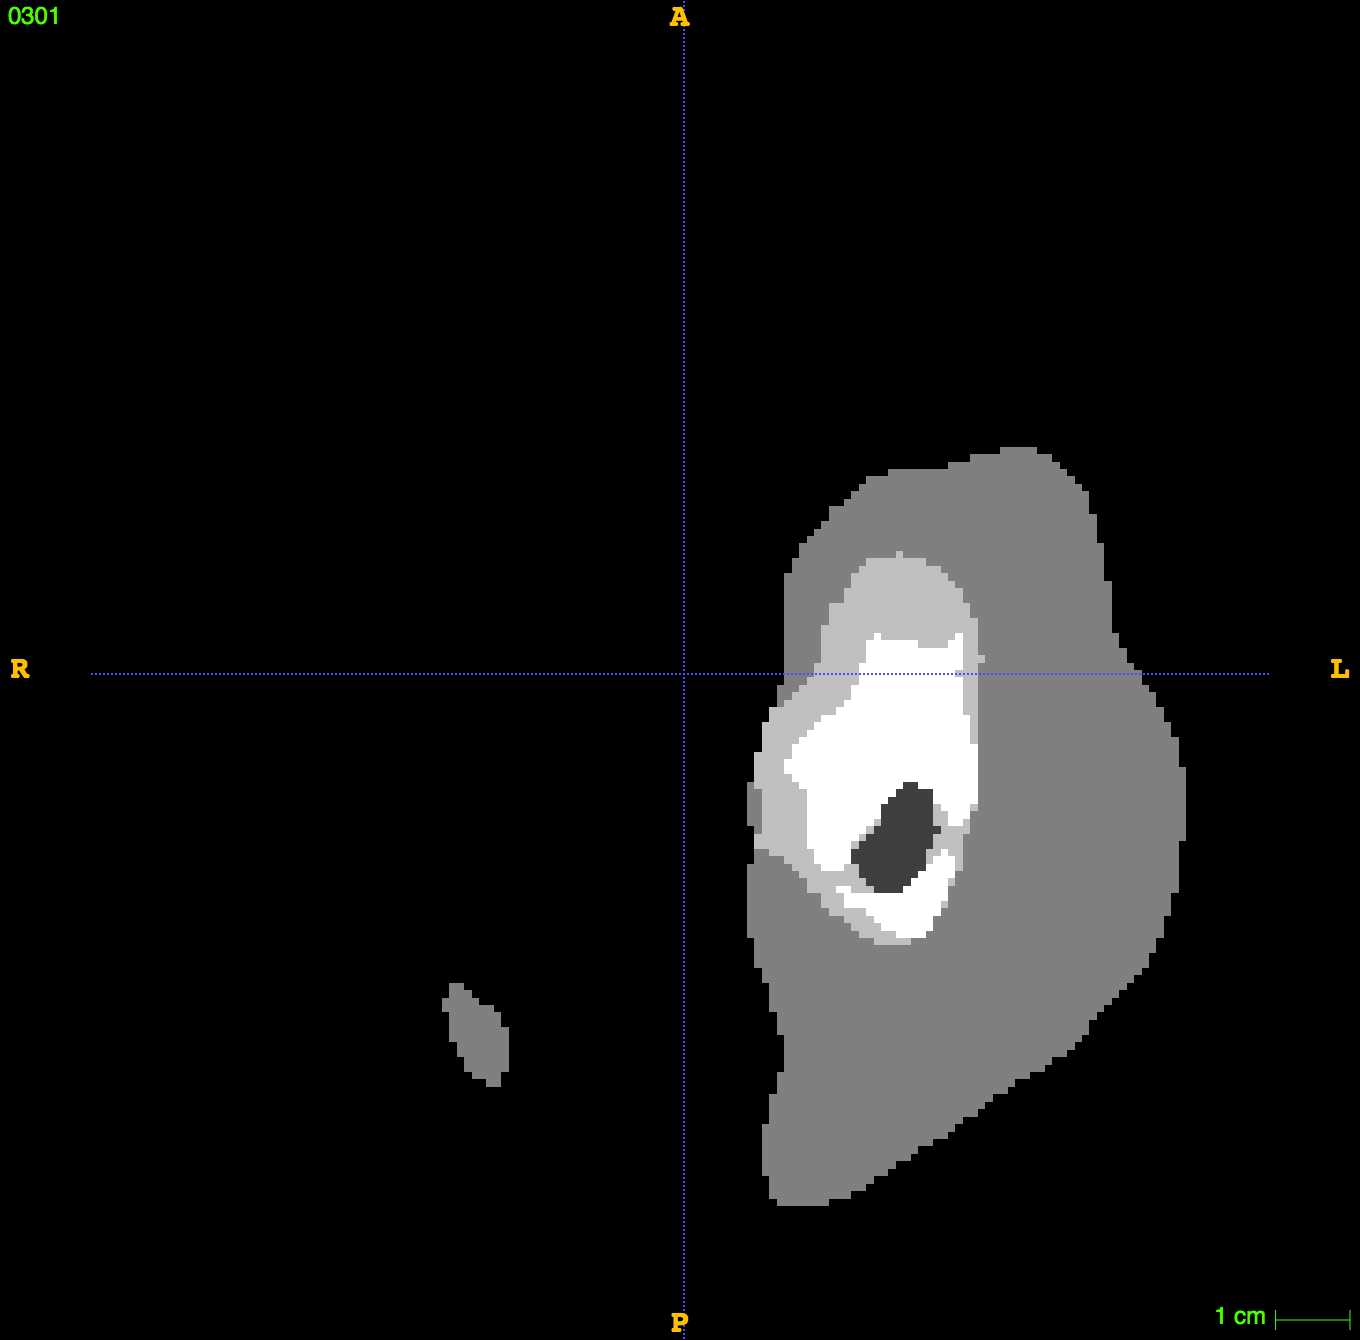
\includegraphics[scale = 0.1]{challenge_1_segmentation_66}
	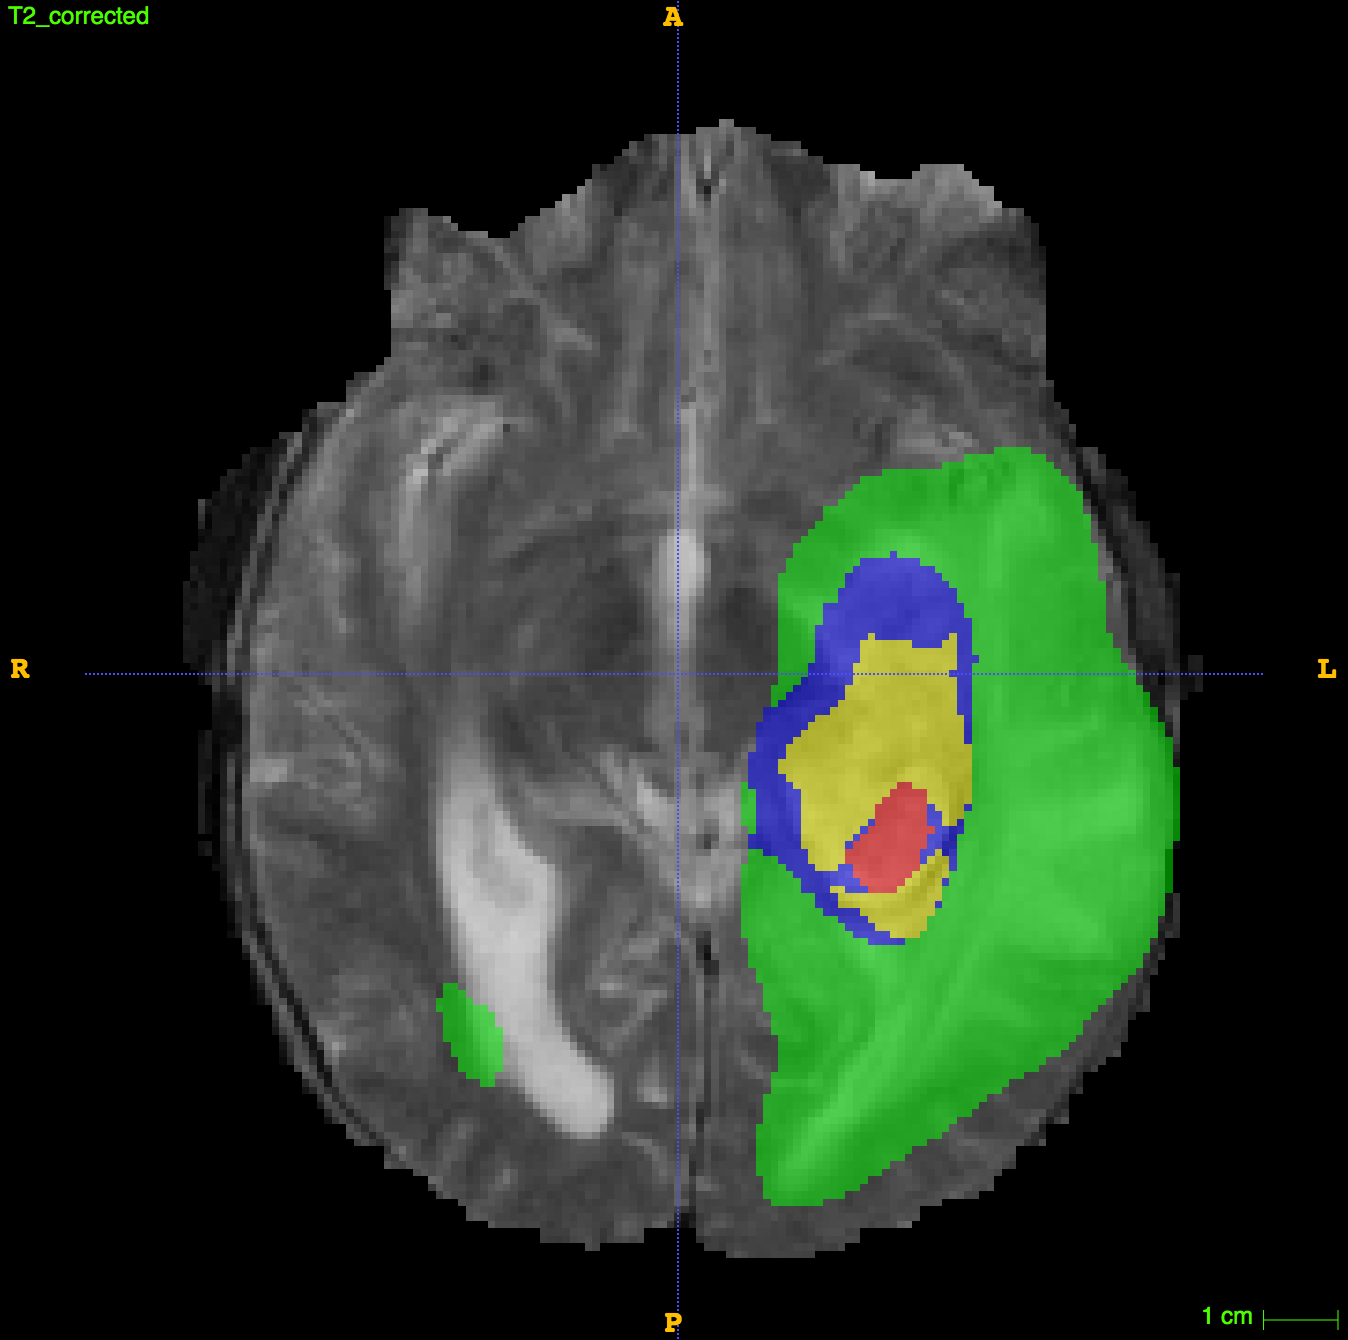
\includegraphics[scale = 0.1]{challenge_1_segmentation_with_T2_66}
	\\
	\vspace{0.5cm}
	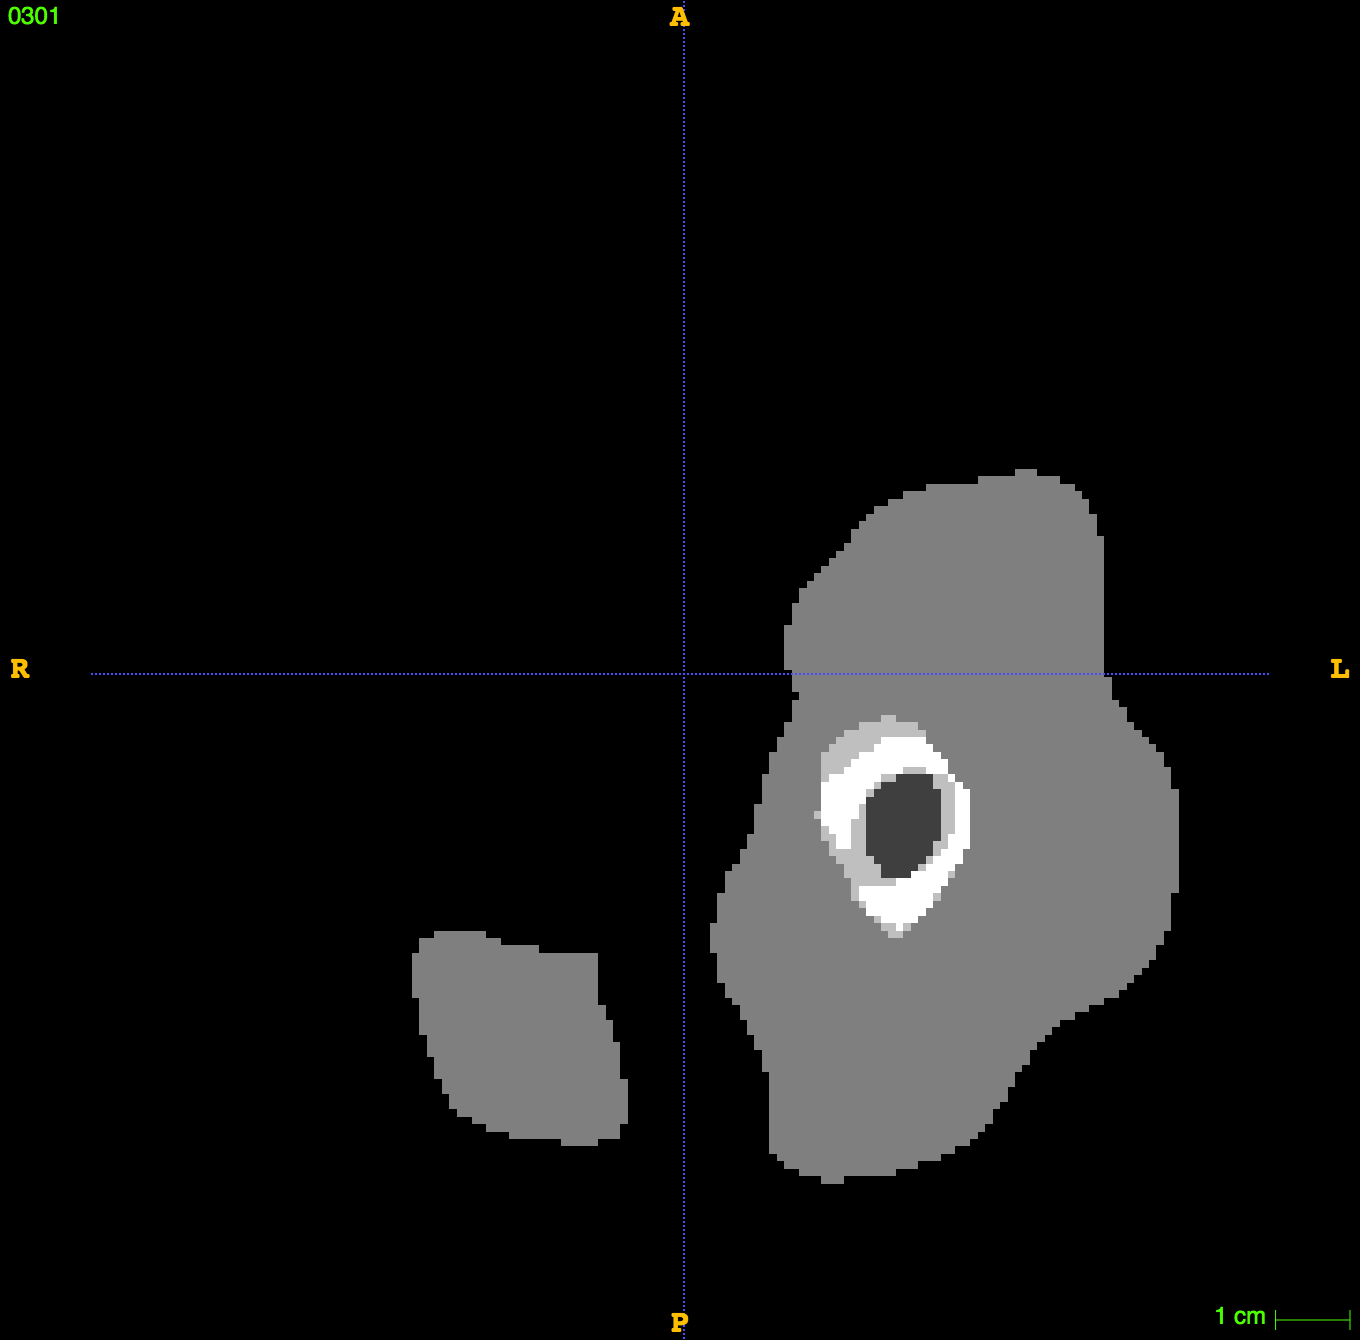
\includegraphics[scale = 0.1]{challenge_1_segmentation_71}
	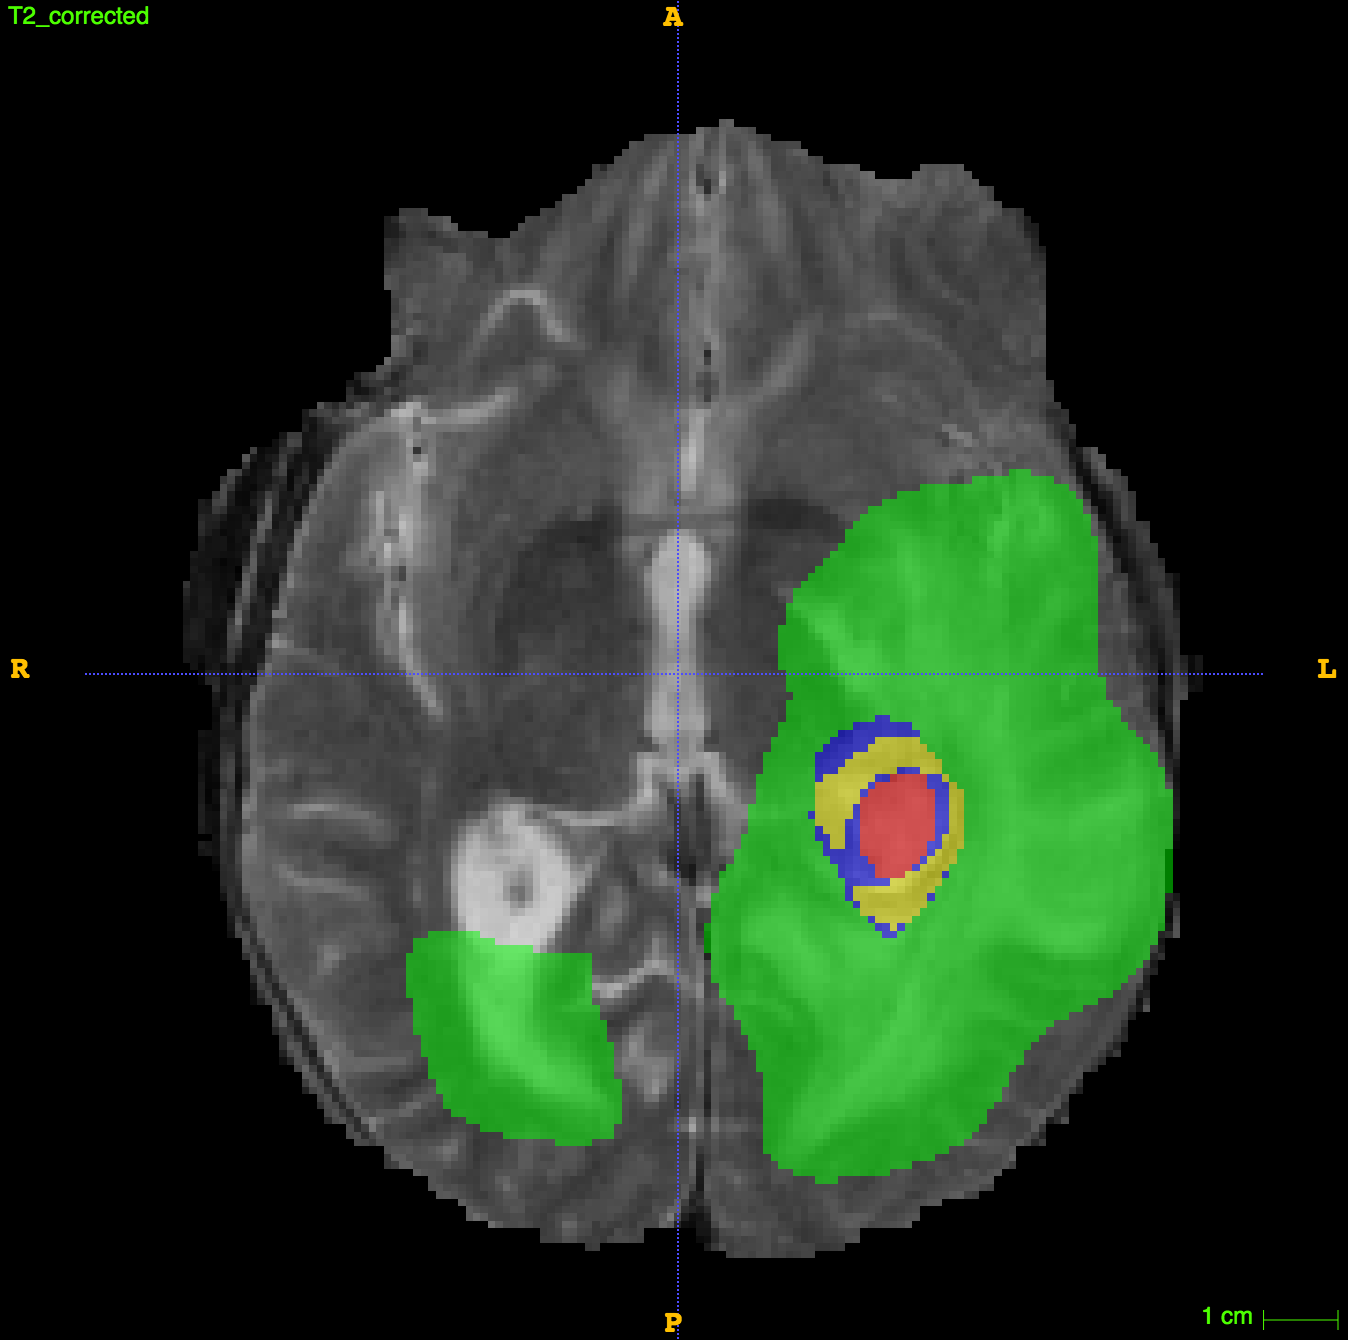
\includegraphics[scale = 0.1]{challenge_1_segmentation_with_T2_71}
	\\
	\vspace{0.5cm}
	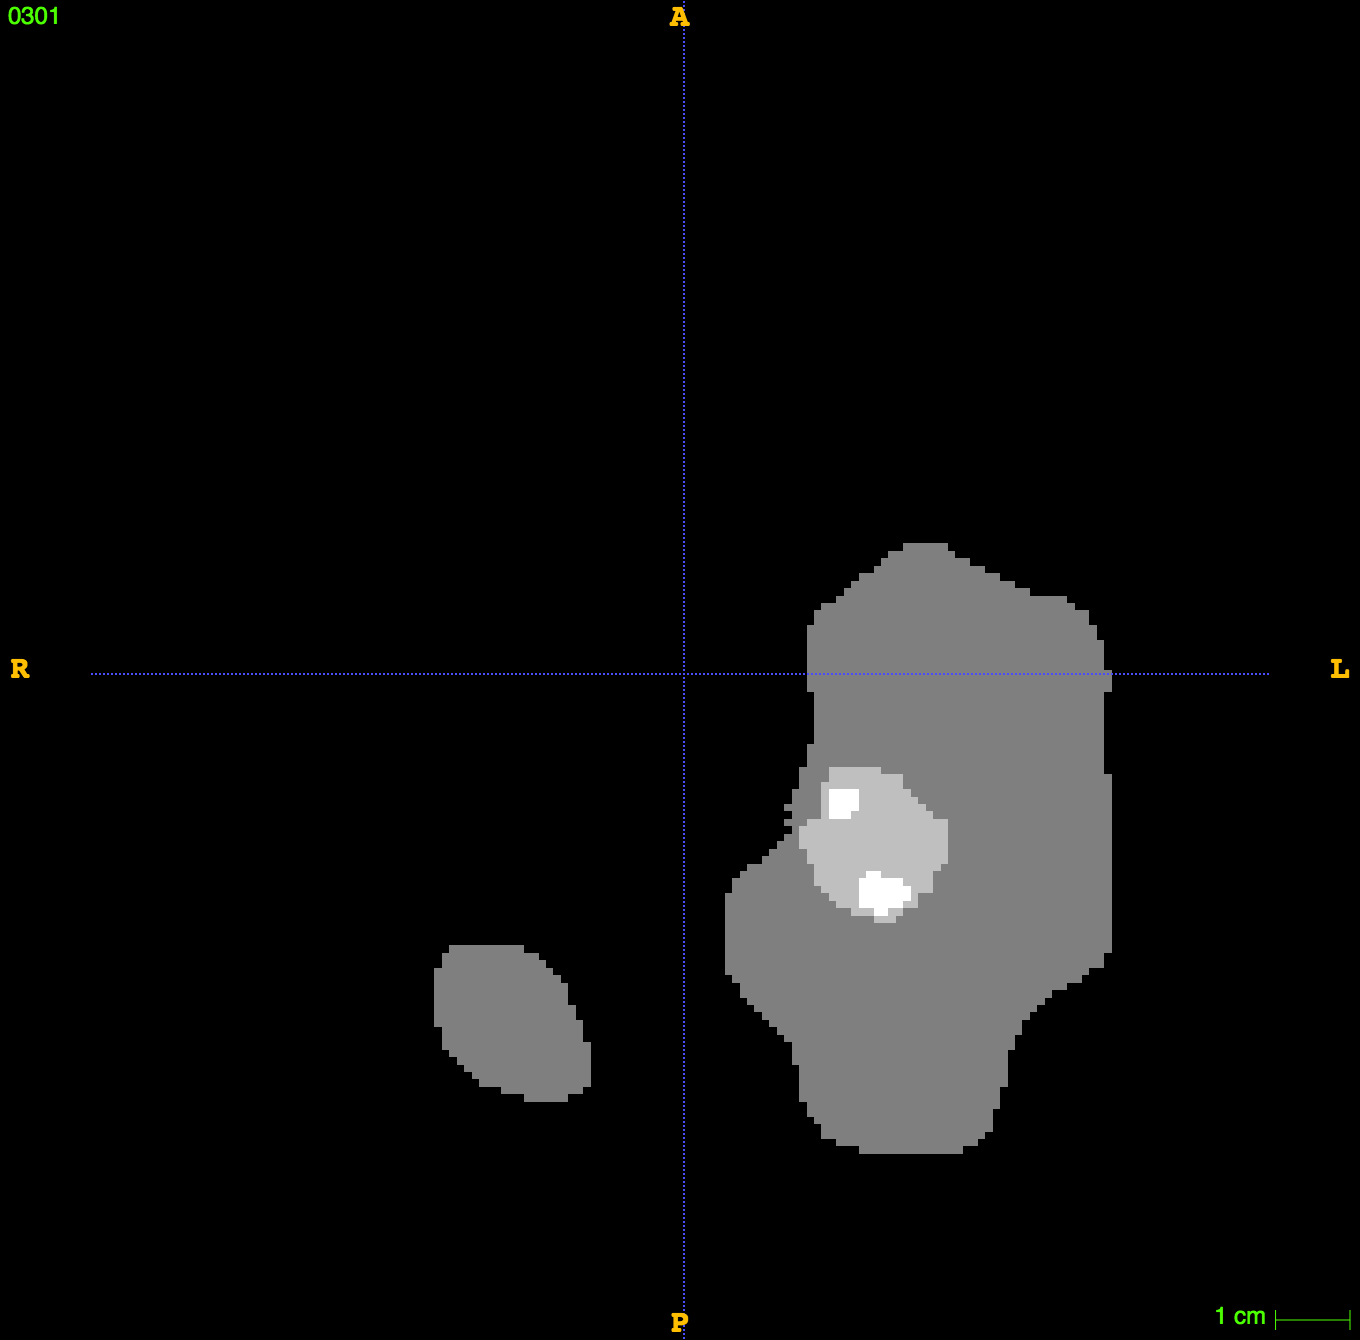
\includegraphics[scale = 0.1]{challenge_1_segmentation_76}
	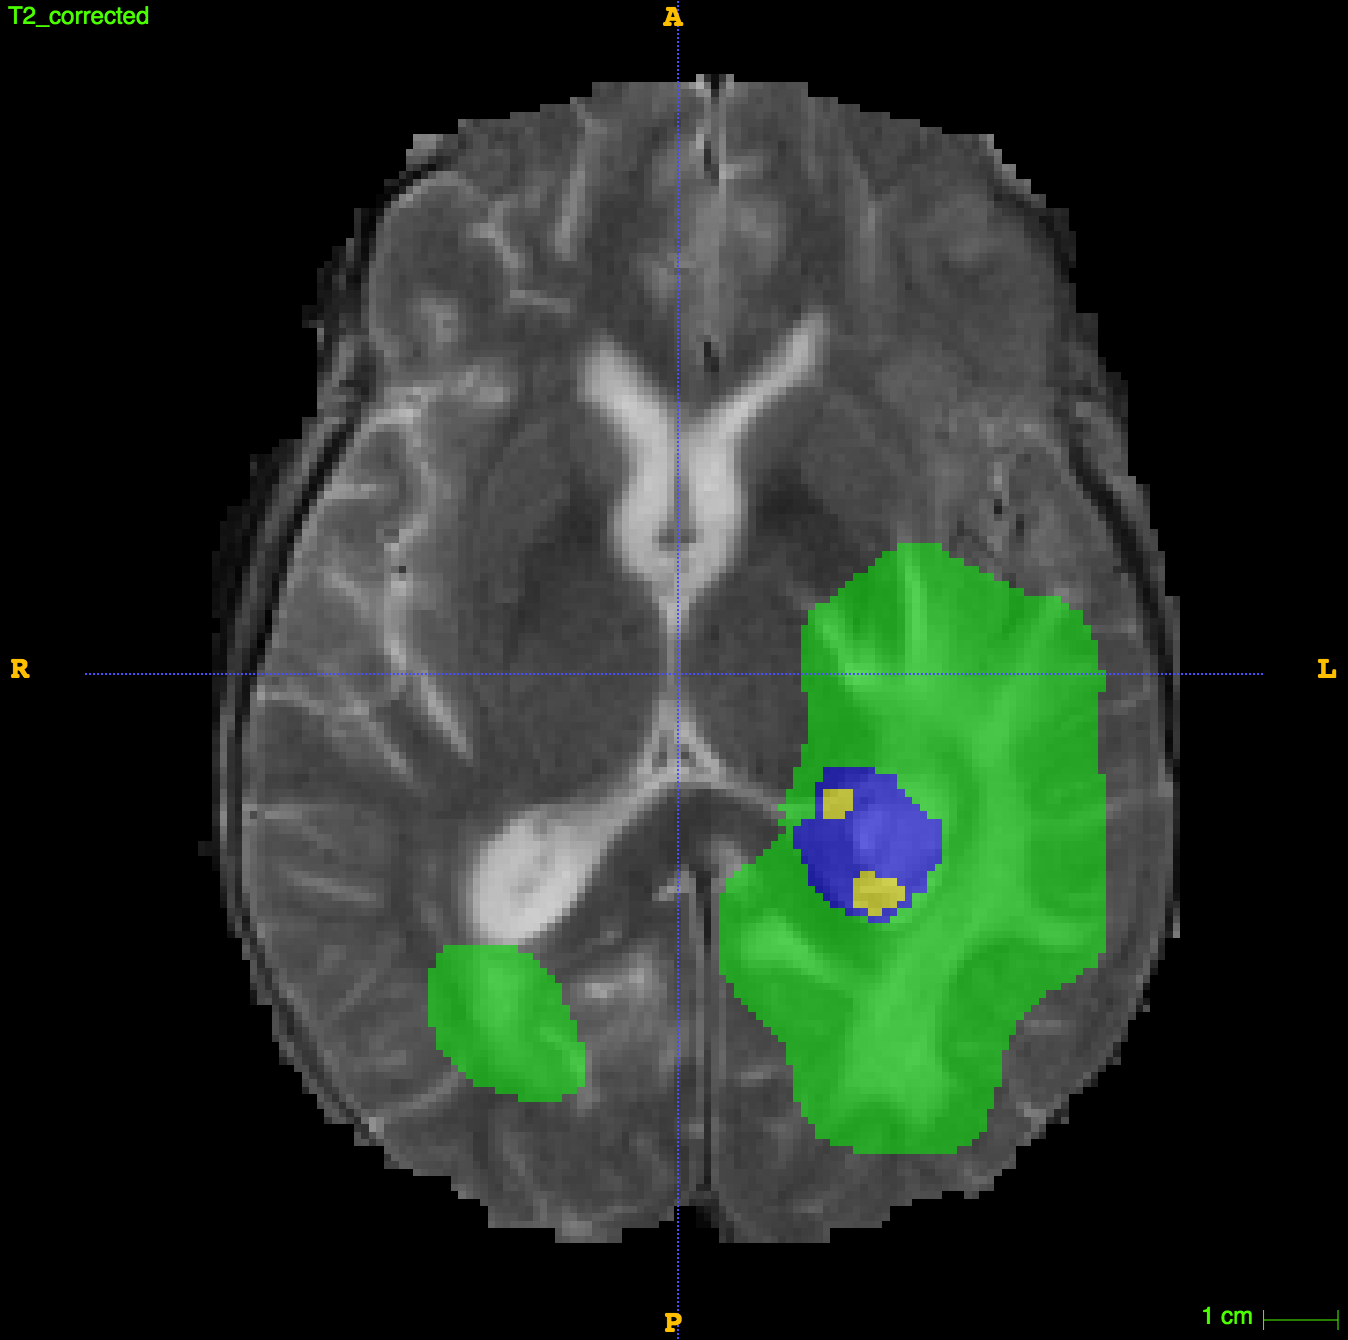
\includegraphics[scale = 0.1]{challenge_1_segmentation_with_T2_76}
	
	\caption[Example segmentation computed using the model proposed by Pereira et al.]{Left column: The segmentation for patient 1 in the challenge dataset for axial plane slices for $z \in \{66, 71, 76\}$. Right column: The same segementation slices overlaid on the T2 scan.}
	\label{fig:example_pereira_segmentation}
\end{figure}

\subsection{My model}
As my model classifies the central $8 \times 8$ voxels for each input patch, the segmentation is slightly more complicated. The padding has to be done differently, as it depends on the size of the image. This is because we are effectively convolving the model on the slices with a stride of $8 \times 8$ and thus the last application of the model in a row or column might not fit if the width or height of the slice is not a multiple of 8. To fix this I pad the end of the x and y axes by an extra 8 voxels. Thus, the model is padded by $\frac{64 - 8}{2} = 28$ zeros in front of the x and y axis and the end is padded with $\frac{64 -8}{2} + 8 = 36$ zeros. Then, for each slice in the image, the steps computed are:
\begin{enumerate}
	\item Extract all patches of size $64 \times 64 \times 4$ for the entire slice, so that the center $8 \times 8$ squares of each patch do not overlap but cover the entire input image. This can be done after padding by two nested for loops with step increments of 8.
	\item Iterate over the patches in batches, such that each batch fits into the memory of the GPU and use the convolutional neural network to predict the class for the central $8 \cdot 8 = 64$ voxels of each patch. These are returned in a one-dimensional array.
	\item Concatenate all the predictions for all batches into a single one-dimensional array of length $64 \cdot \#patches$. This one-dimensional array has to be transformed back into a two-dimensional array such that each voxel is mapped back into its original position in the input image.
	\item Calculate the number of patches that fit into the slice as follows:
		\begin{equation}
		\begin{split}
			\text{height}_p & \gets \bigg \lceil \cfrac{\text{image\_height}}{8} \bigg \rceil 	 \\
			\text{width}_p & \gets \bigg \lceil \cfrac{\text{image\_width}}{8} \bigg \rceil 	 \\
		\end{split}		
		\end{equation}
	\item Reshape the voxels into a single 4-dimensional array of size $(\text{height}_p \times \text{width}_p \times 8 \times 8)$
	\item Concatenate the array along its first axis. This can be done using the \texttt{concatenate} function provided by numpy. The result is a 3-dimensional array of size $(\text{height}_p \times 8 \cdot \text{width}_p \times 8)$. This will concatenate individual patches along rows together.
	\item Similarly, concatenate the new array along its first axis. This will concatenate the columns, resulting into a single 2-dimensional array of size $(8 \cdot \text{height}_p \times 8 \cdot \text{width}_p)$.
	\item Finally, remove the extra voxels that might have been added by the extra padding. This can be done using numpy to trim the array to the image width and height. The result will be a 2-dimensional array which is the segmented slice.
\end{enumerate}


\section{Segmentation post-processing}
After the new patient has been segmented, a further simple heuristic is used to remove small volumes of data labeled as non normal tissue, based on the assumption that the diseased tissue be connected into a single component of relatively large size. Pereira et al \cite{pereira} proposed to remove all connected components (continuous regions of diseased tissue) of less than 10,000 voxels in volumes.

I implement this heuristic using a depth first search on the graph represented by a scan, where each voxel is a vertex and shares an edge with its 6 immediate neighbours (or less if it is on an edge). First, I create a second 3-dimensional array of the same size as the scan. This array will be used to mark which nodes have already been visited and processed. As I only care about the diseased tissue, i.e.\ classes 1--4, I mark all voxels with a 1 for which the corresponding voxel in the segmentation has value 0. Then the algorithm iterates the following steps until all voxels have been visited:
\begin{enumerate}
	\item Initialise an empty list, to represent the next connected component $C$.
	\item Remove a previously not visited voxel, mark it as visited, add its coordinates to $C$.
	\item Initialise a queue containing all non visited neighbours of the voxel that are not segmented as normal tissue. Mark the neighbours as visited.
	\item Then, repeat while the queue is not empty:
	\begin{enumerate}
		\item Pop the first element, mark it as processed, and add its coordinates to the connected component $C$.
		\item Find its neighbours that have not been visited or processed. Mark those as visited and push those to the end of the queue. Repeat step 4.
	\end{enumerate}
	\item Once the queue is empty, add the connected component $C$ to a list containing all disjoint connected components.
\end{enumerate}
Finally, I iterate over the list of connected components, finding those which have less voxels than the threshold size and setting the segmentation of those voxels to 0. Figure \ref{fig:connected_components_example} shows the effect of applying this post-processing step to the last challenge scan.
\begin{figure}[h]
	\centering
	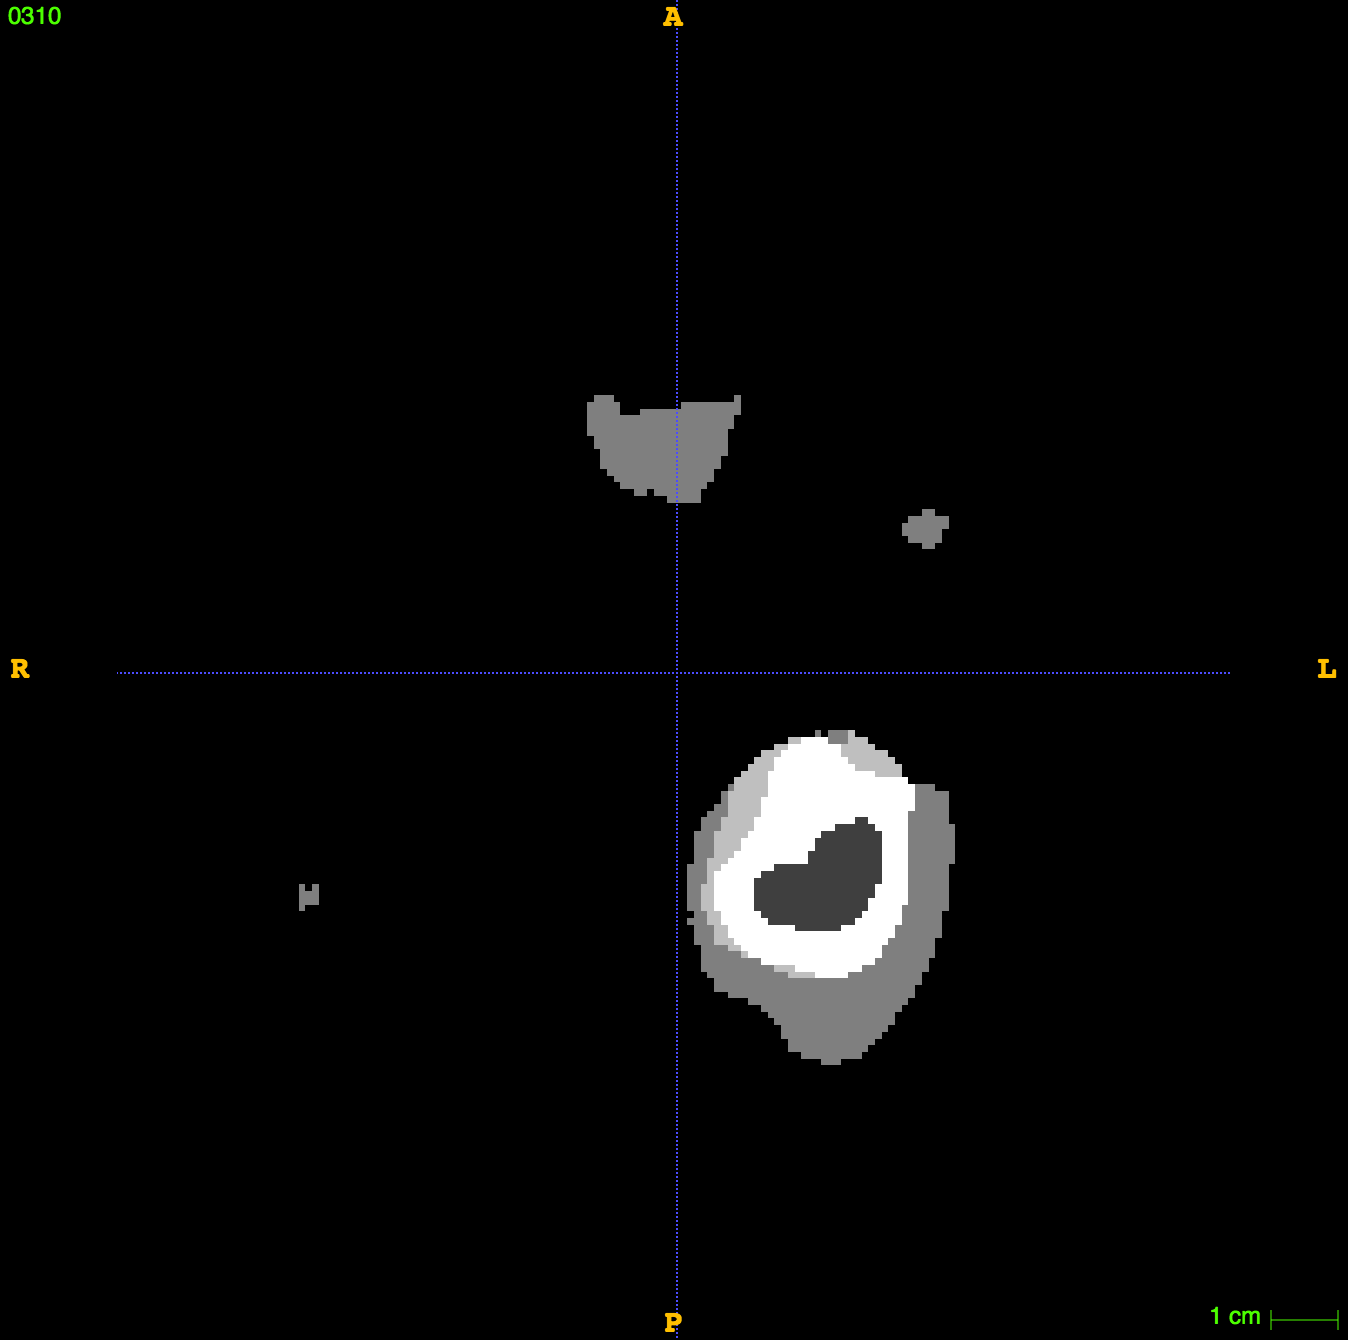
\includegraphics[scale = 0.1]{challenge10_no_post_77}
	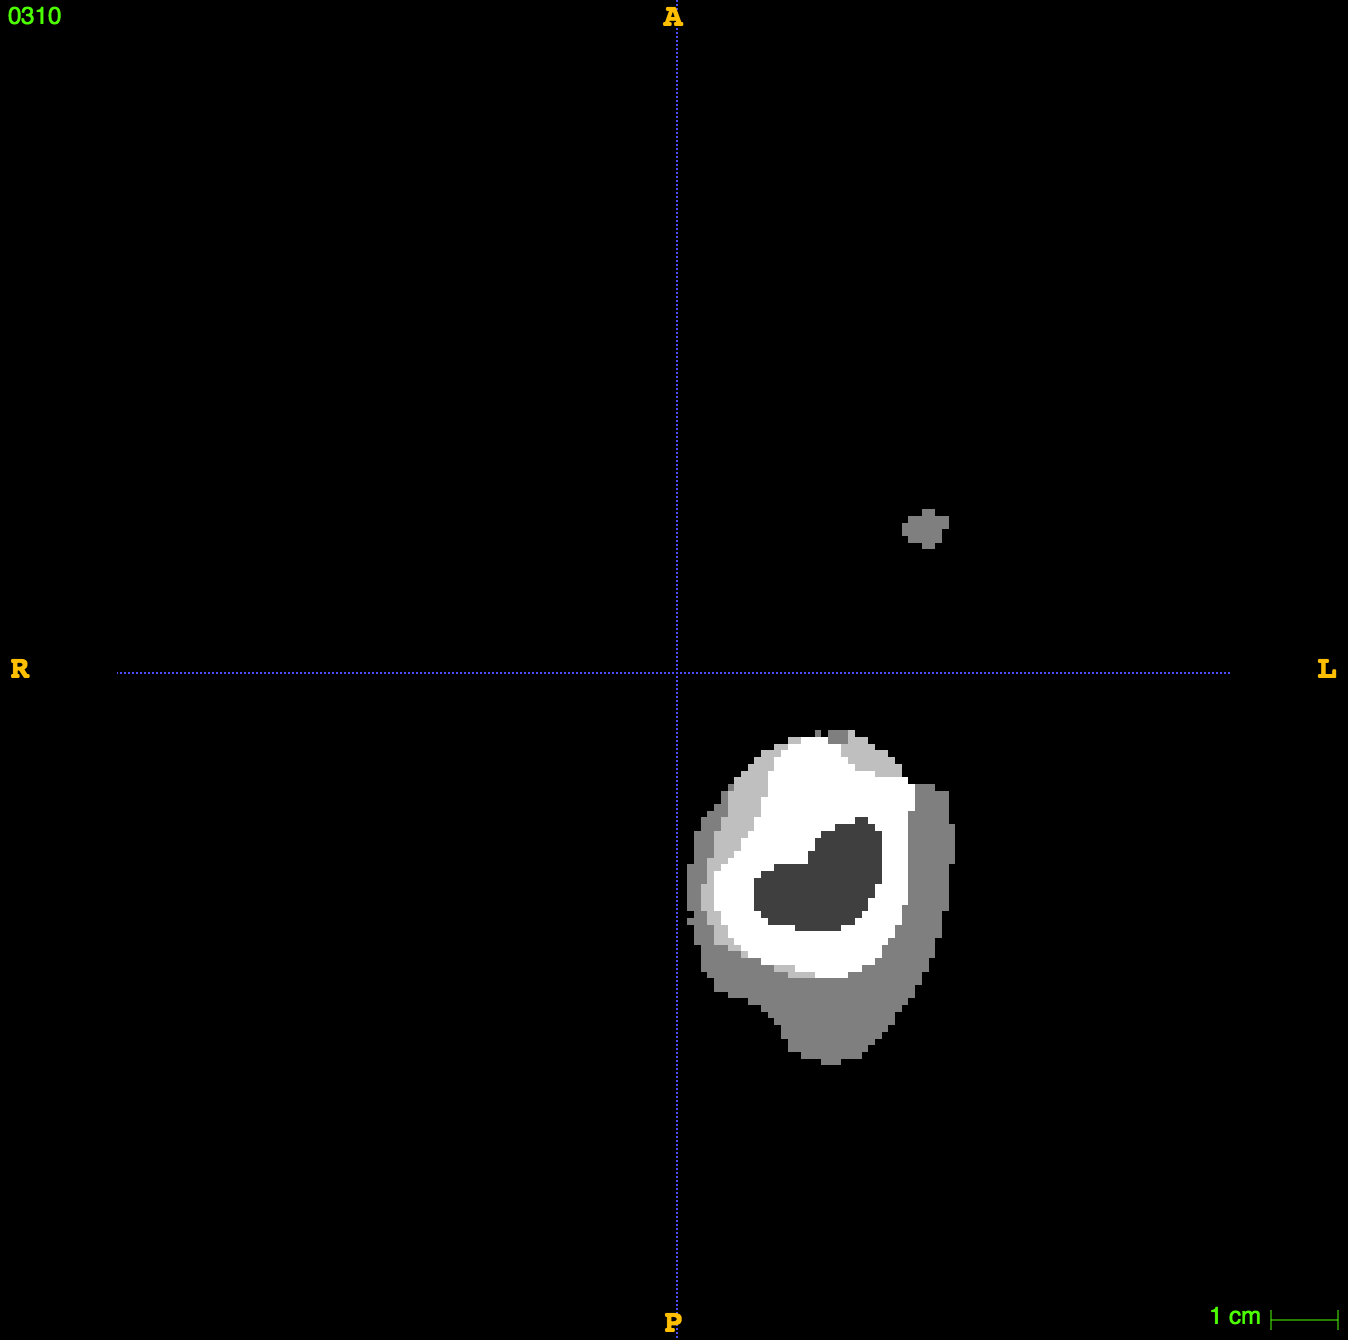
\includegraphics[scale = 0.1]{challenge10_with_post_77}
	\\
	\vspace{0.5cm}
	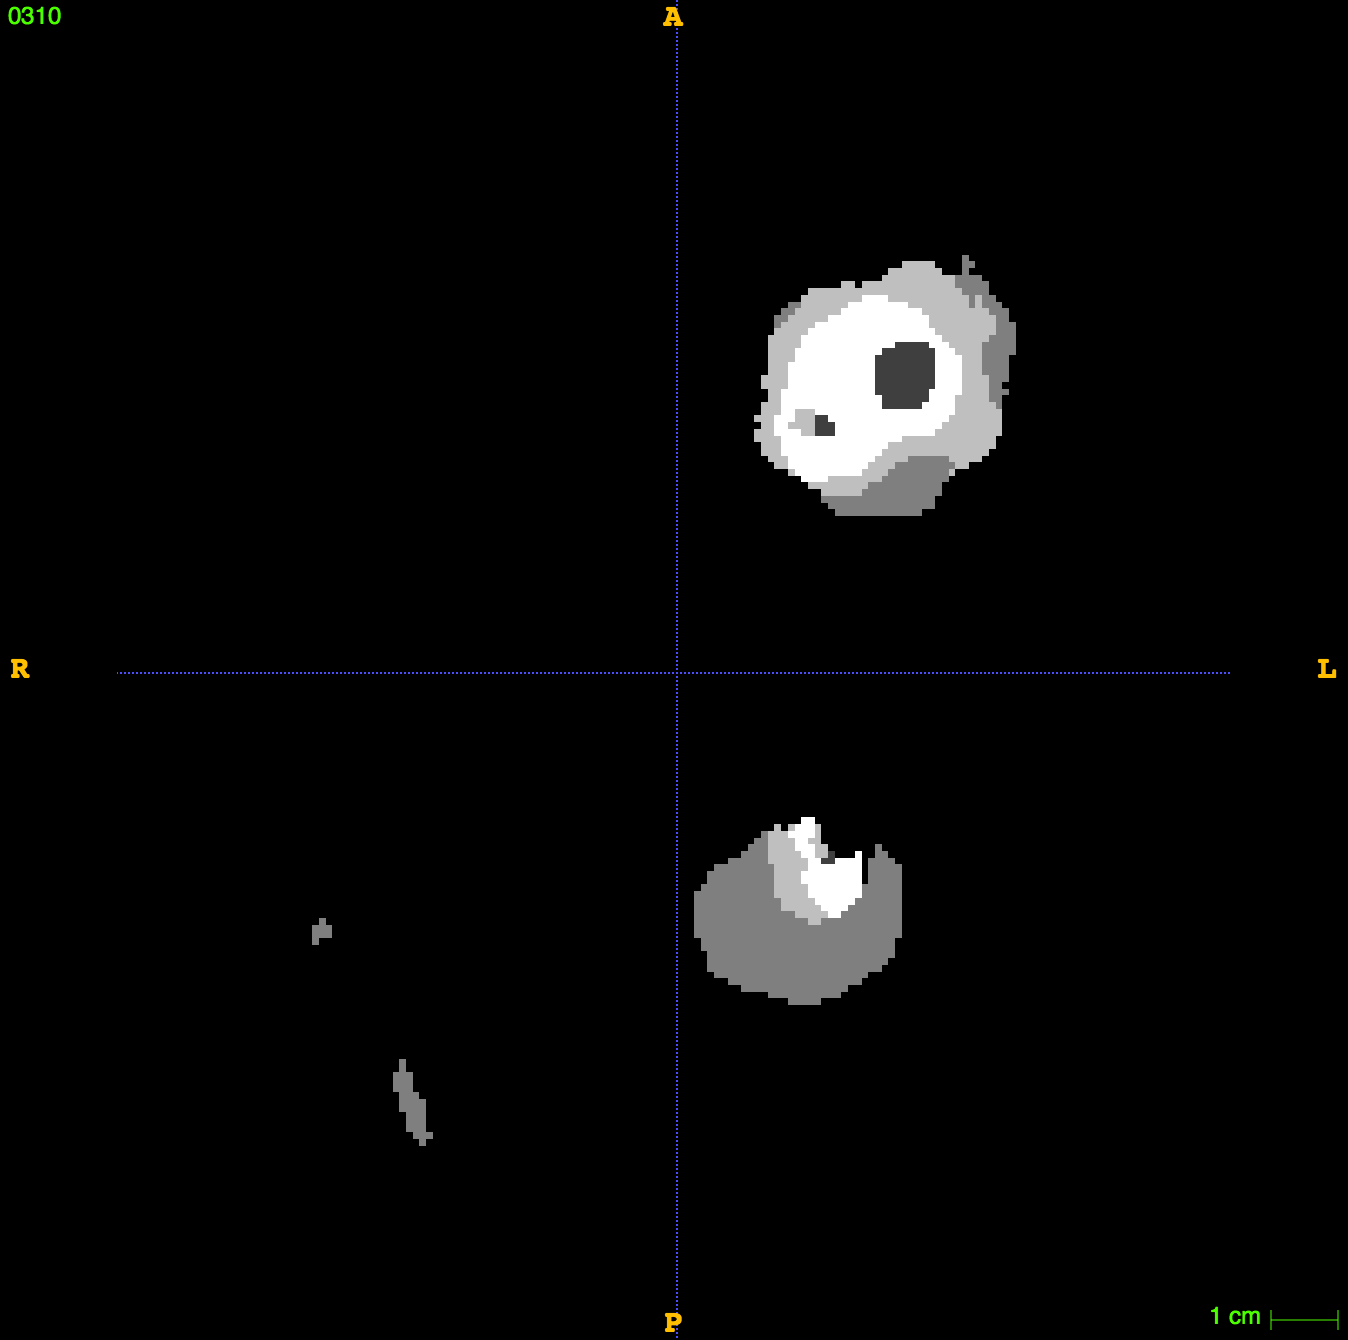
\includegraphics[scale = 0.1]{challenge10_no_post_87}
	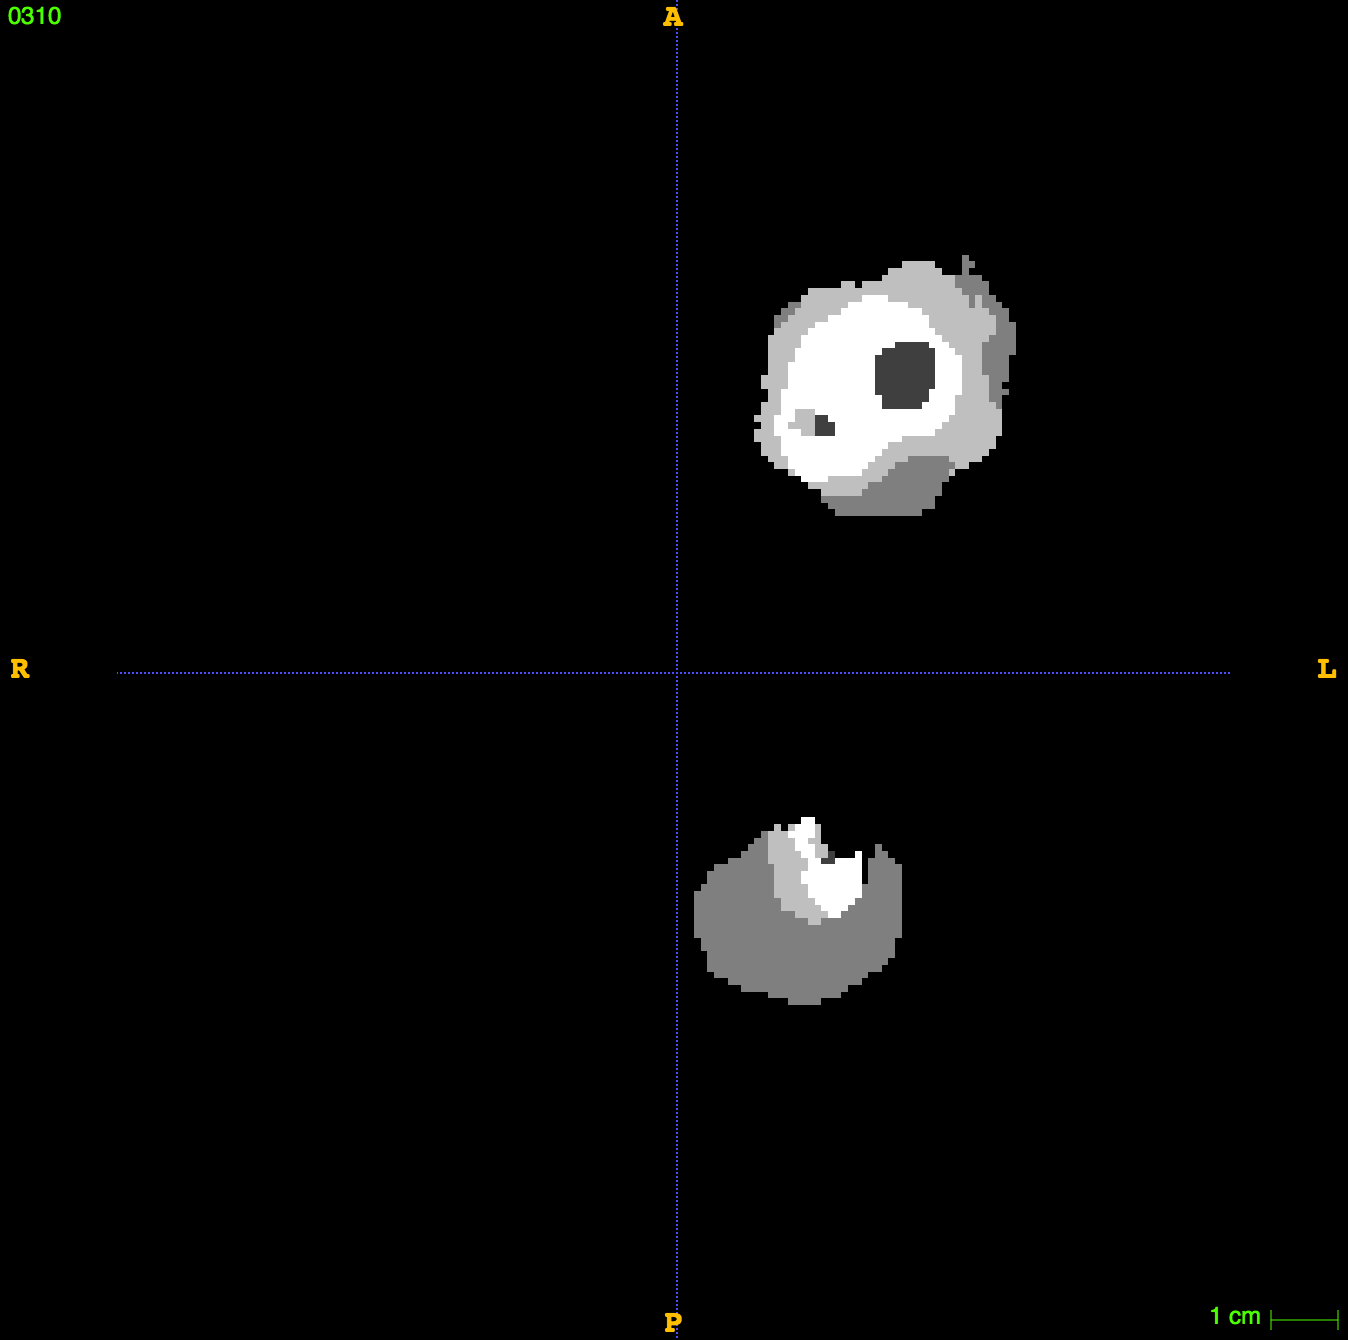
\includegraphics[scale = 0.1]{challenge10_with_post_87}
	\caption[Effect of applying the post-processing step]{Effect of applying the post-processing step to the 10\textsuperscript{th} challenge scan. Axial plane slices $z \in \{77,87\}$ are shown side-by-side (on the left before the post-processing step and on the right with the post-processing step).}
	\label{fig:connected_components_example}
\end{figure}

\chapter{Evaluation}

\section{Unit Tests}
To verify that the stages behave as expected, I implement some unit tests using the Python inbuilt \texttt{unittest}\footnote{\url{https://docs.python.org/3/library/unittest.html}} module as it does not require any additional libraries. Furthermore, the module was inspired by JUnit, which I had previously used during other projects.

 For the normalisation stage, I used the ANTs neuroimaging tools and scipy to perform the N4 correction and the winsorising step respectively, thus I only test the mean and standard deviation normalisation. I test the patch extraction phase with small 4-dimensional arrays, for which I can test that the correct patches are returned and that the patch labels are balanced. The data augmentation stage does not need to be unit tested as it is implemented with a Keras `data generator'. I test the segmentation stage similarly, using small arrays and a simple classifying function to mock the behaviour of the convolutional neural network. Finally, I also test the post-processing stage for different inputs with known outputs.
 
As an example, I include two of the tests for the post-processing step:
\begin{lstlisting}[language=Python]
	class TestRemoveConnectedComponents(unittest.TestCase):

    def test_no_components(self):
        image = np.full(shape=(3,3,3), fill_value=0)
        image2 = np.copy(image)
        remove_connected_components(image2, 1, verbose=False)
        self.assertTrue(np.array_equal(image, image2))
    
    def test_remove_one_component(self):
        image = np.array([[[0,0,0],[0,0,0],[0,0,0]],
                          [[0,0,0],[0,1,0],[0,0,0]],
                          [[0,0,0],[0,0,0],[0,0,0]]])
        remove_connected_components(image, 2, verbose=False)
        self.assertTrue(np.array_equal(image, np.full(image.shape, 0)))
\end{lstlisting}

Figure \ref{fig:unit_test_output} shows the output of running the unit tests. All unit tests pass, indicating that the tested stages behave as expected.

\begin{figure}
	\centering
	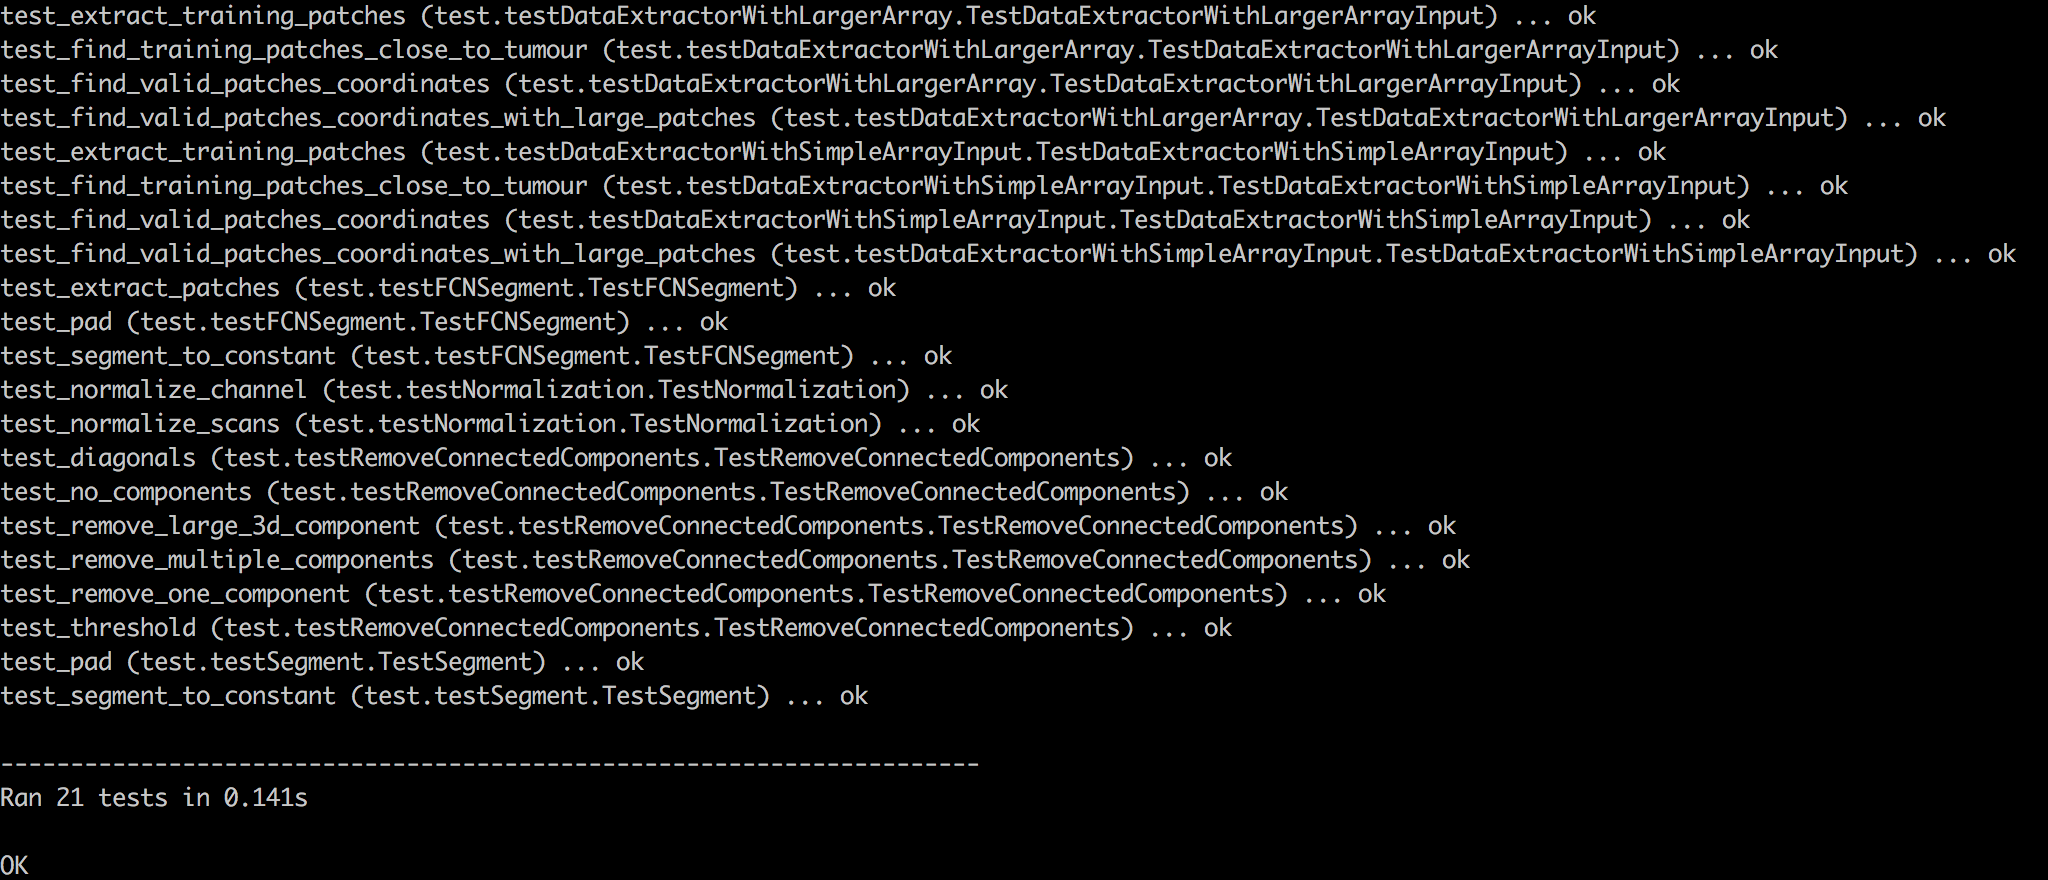
\includegraphics[width = \textwidth]{unit_test_output}
	\label{fig:unit_test_output}
	\caption{Output of running the unit tests. All tests pass successfully.}
\end{figure}

\section{BraTS evaluation}
\subsection{Evaluation metrics}
The BraTS2013 challenge \cite{brats-proceedings} evaluates the segmentation using three different metrics: \textbf{dice score}, \textbf{sensitivity} (also referred to as recall) and \textbf{positive predictive value} (also referred to as precision). These metrics are best visualised using the Venn diagram shown in figure \ref{fig:evaluation_venn_diagram}.  Note in particular, that accuracy metric is not used. This is because the data is highly unbalanced, as shown previously, meaning that a model trivially labelling everything with class 0 would reach an accuracy of 99\% or more, making it very hard to compare different models.

\begin{figure}
	\centering
	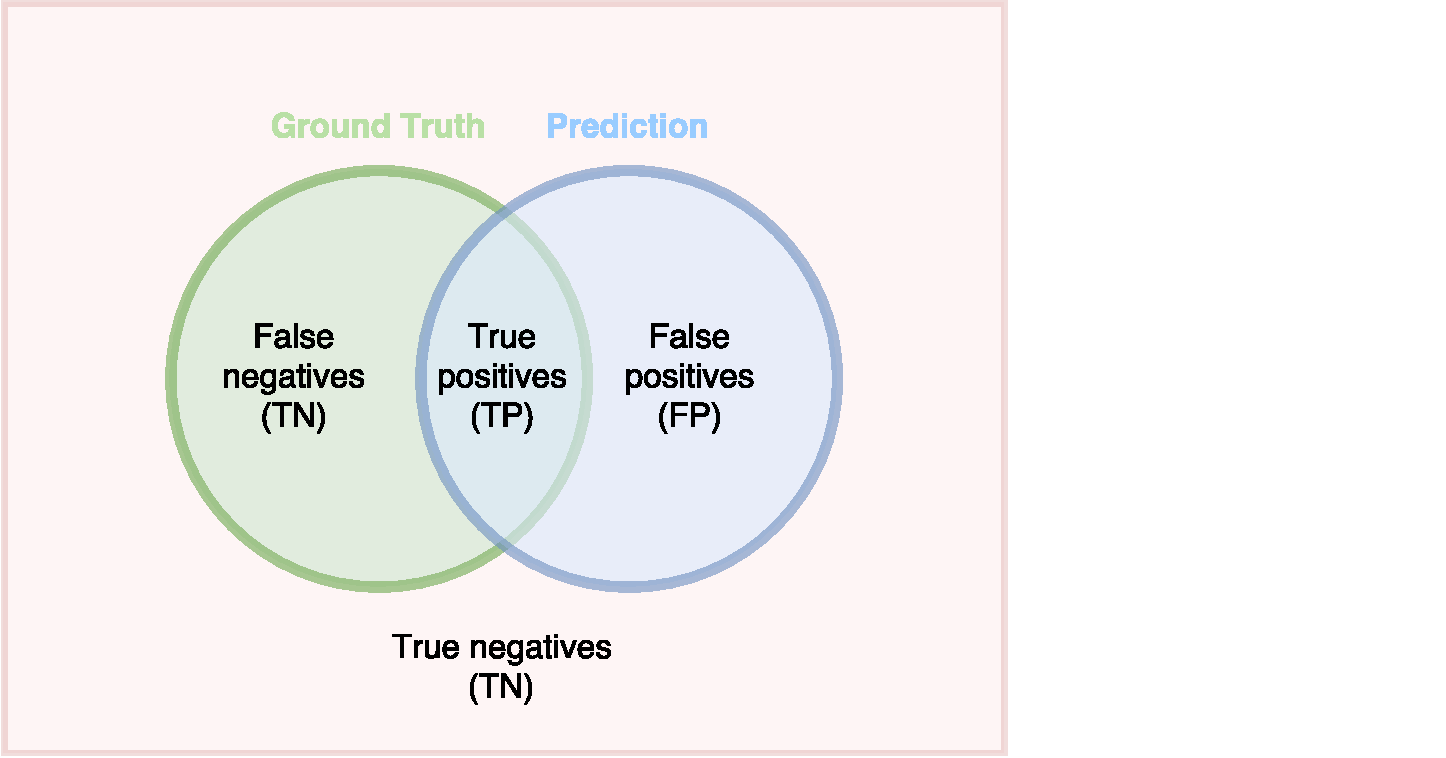
\includegraphics[scale = 0.5]{evaluation_venn_diagram}
	\label{fig:evaluation_venn_diagram}
	\caption{Venn diagram showing the different areas and how the can be classified.}
\end{figure}

\subsubsection{Positive predictive value}
The positive predictive value is defined as
\begin{equation}
	\textrm{PPV} = \frac{\textrm{TP}}{\textrm{TP} + \textrm{FP}}
\end{equation}
where \textrm{TP} and \textrm{FP} are the numbers of true and false positives respectively. In the Venn diagram \ref{fig:evaluation_venn_diagram}, this corresponds to the size of the green and blue area relative to the size of the entire blue area.  Since the denominator $\textrm{TP} + \textrm{FP}$ is the total number of positively classified elements, the positive predictive value gives an indication as to how accurately the model can predict a positive class. In the case of brain tumour segmentations, the positive predictive value measures how confidently the model is predicting tumours, with a high positive predictive value meaning that regions labelled as tumours by the model really tumours are.
\subsubsection{Sensitivity}
The sensitivity is defined as 
\begin{equation}
	\textrm{Sensitivity} = \frac{\textrm{TP}}{\textrm{TP} + \textrm{FN}}
\end{equation}
where \textrm{FN} is the number of false negative classifications and \textrm{TP} is the number of true positives. The sensitivity measures the size of the blue and green region relative to the size of the entire green region. As the denominator $\textrm{TP} + \textrm{FN}$ equals the green area, i.e.\ the total number of positively labelled elements in the ground truth, the sensitivity measures how well a model is able to recognise positively labelled examples. In the case of brain tumour segmentations, the sensitivity measures how good a model is at recognising a tumour. A high sensitivity would indicate that the model is able to recognise a high fraction of the positively labelled voxels.

\subsubsection{Trade-off between positive predictive value -- Sensitivity }
There is a trade-off between the sensitivity and the positive predictive value. A model classifying everything as negative would reach perfect positive predictive as there would be no false positives but would have a sensitivity of 0. Similarly, a model classifying everything as positive would reach perfect sensitivity as there would be no false negatives but would have a positive predictive value of 0. For brain tumours, a high sensitivity is arguably more important as missing a tumour can have deadly consequences. However, this has a trade-off with the utility of a model, since a low positive predictive value also means that we can only have little confidence in the positive predictions made by it.

\subsubsection{Dice score}
The dice score takes into account both the false negatives and the false positives and thus give a metric which is to some extend independent of that trade-off. The dice score is defined as
\begin{equation}
\begin{split}
	\textrm{Dice Score} & = \cfrac{\vert \textrm{Ground truth} \cap \textrm{Prediction}\vert}{\frac{1}{2} \cdot (\vert \textrm{Ground truth}\vert + \vert \textrm{Prediction}\vert)} \\
	&  = \cfrac{2 \cdot \textrm{TP}}{\textrm{FP} + 2 \cdot \textrm{TP} + \textrm{FN}}
\end{split}
\end{equation}
The dice score normalises the number of true positive classification to the average size of the two segmented areas.

Figure \ref{fig:evaluation_example} shows a fictive example for a segmented slice in the axial plane.  The metrics for this segmentation are
\begin{equation*}
\begin{split}
	\textrm{PPV} & = \cfrac{\vert P_1 \cup T_1 \vert}{\vert P_1 \vert} \\
	\textrm{Sensitivity} & = \cfrac{\vert P_1 \cup T_1 \vert}{\vert T_1 \vert} \\
	\textrm{Dice score} & = \cfrac{\vert P_1 \cup T_1 \vert}{\frac{1}{2} \cdot (\vert P_1 \vert + \vert T_1 \vert)} \\
\end{split}
\end{equation*}

\begin{figure}[h]
	\centering
	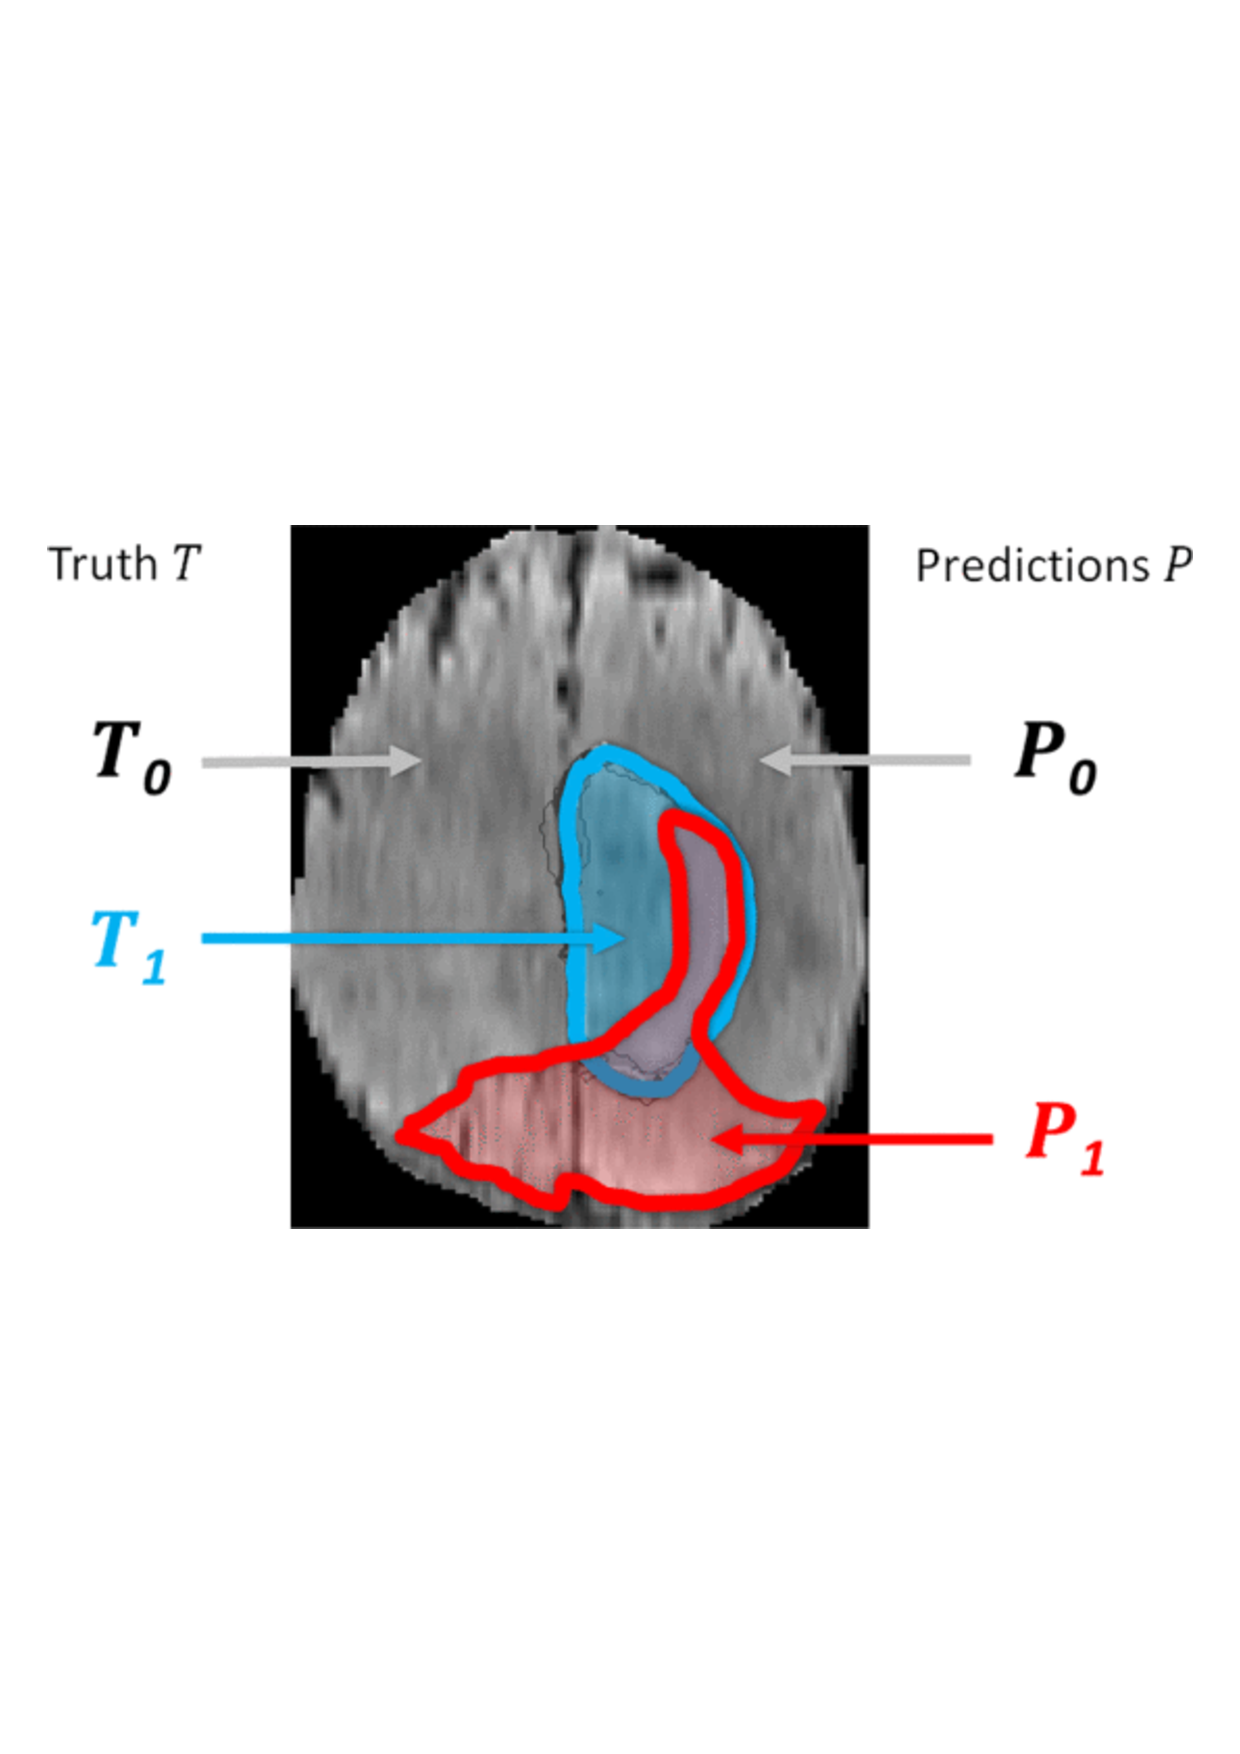
\includegraphics[scale = 0.5]{example_evaluation}
	\label{fig:evaluation_example}
	\caption{Example showing a segmentation for a slice in the axial plane. This image was reproduced from \cite{brats-proceedings}}
\end{figure}

\subsection{Regions of evaluation}
As stated above, the metrics are defined only for binary classification into positive and negative classes. However, our segmentations are classified into 5 different classes (0--4). Therefore, different `regions' define which classes are counted as positive and which ones as negative. For the BraTS challenge there are three regions:
\begin{enumerate}
	\item \textbf{Complete}: All classes 1--4 are defined as positive, only 0 as negative. The metrics for the complete scores therefore evaluate how well a model is able to discern diseased tissues from normal tissues.
	\item \textbf{Core}: Classes 1,3 and 4 are defined as positive, 0 and 2 as negative. In this region, the edema class is no longer considered as positive.
	\item \textbf{Enhancing} Only class 4, the enhacing tumour class is defined as positive. The metrics for this region measure how well the model can segment the enhancing tumour class only.
\end{enumerate}


\section{Evaluation of the model proposed by Pereira et al.}
\subsection{BraTS evaluation}
In table \ref{table:pereira_dice_results} are shown the Dice score values I obtained for each of the 10 challenge scans using the method proposed by Pereira et al.\ \cite{pereira}. In figure \ref{pereira_box_plot} the mean and standard deviation are plotted for the three regions along with the minimum and maximum values. \begin{table}
\centering	
\begin{tabular}{ c | c c c} 
\multirow{2}{*}{\textbf{Patient}} & \multicolumn{3}{c}{\textbf{Dice score}} \\
 & Complete & Core & Enhancing \\
 \hline
1 & 0.813 & 0.843 & 0.472 \\
2 & 0.796 & 0.700 & 0.619 \\
3 & 0.808 & 0.765 & 0.345 \\
4 & 0.723 & 0.426 & 0.178 \\
5 & 0.750 & 0.676 & 0.550 \\
6 & 0.776 & 0.510 & 0.518 \\
7 & 0.818 & 0.035 & 0.034 \\
8 & 0.829 & 0.878 & 0.700 \\
9 & 0.881 & 0.883 & 0.818 \\
10 & 0.852 & 0.840 & 0.840 \\
\hline
\rule{0pt}{3ex}    
\textbf{mean} & $0.805 \pm 0.047$ & $0.656 \pm 0.267$ & $0.508 \pm 0.262$
\end{tabular}
\caption{Dice scores obtained for the 10 challenge patients using the method proposed by Pereira et al. These results were produced by the online evaluation platform as the ground truth labelling is not publicly available.}
\label{table:pereira_dice_results}
\end{table}

\begin{figure}
	\centering
	\setlength\figureheight{10cm}
	\setlength\figurewidth{0.8\textwidth}
	% This file was created by matplotlib2tikz v0.6.6.
\begin{tikzpicture}

\begin{axis}[
xmin=0, xmax=4,
ymin=0, ymax=1,
axis on top,
width=\figurewidth,
height=\figureheight,
xtick={1,2,3},
xticklabels={Complete,Core,Enhancing},
tick pos=both,
legend style={at={(0.03,0.03)}, anchor=south west},
legend cell align={left},
legend entries={{Min value},{Max value},{Mean value with std}}
]
\path [draw=blue] (axis cs:1,0.757997136612514)
--(axis cs:1,0.851199263387485);

\path [draw=blue] (axis cs:2,0.388105524055728)
--(axis cs:2,0.923100175944272);

\path [draw=blue] (axis cs:3,0.24529284371699)
--(axis cs:3,0.76972003628301);

\addplot [blue, mark=-, mark size=3, mark options={solid}, only marks]
table {%
1 0.757997136612514
2 0.388105524055728
3 0.24529284371699
};
\addplot [blue, mark=-, mark size=3, mark options={solid}, only marks]
table {%
1 0.851199263387485
2 0.923100175944272
3 0.76972003628301
};
\addplot [blue, mark=*, mark size=3, mark options={solid,draw=black}, only marks]
table {%
1 0.8045982
2 0.65560285
3 0.50750644
};
\addplot [red, mark=x, mark size=3, mark options={solid}, only marks]
table {%
1 0.72251
2 0.0349435
3 0.0343374
};
\addplot [red, mark=x, mark size=3, mark options={solid}, only marks]
table {%
1 0.881144
2 0.88342
3 0.840119
};
\end{axis}

\end{tikzpicture}
	\caption{Box plot showing the dice scores obtained by my implementation of the model proposed by Pereira et al.}
	\label{pereira_box_plot}
\end{figure}

The mean scores for the `Core' and `Enhancing' region are significantly lower than the mean score for the `Complete' region and have a much higher standard deviation. This can partially be explained by the outlier values obtained from patient 7. For this patient, the diseased tissue has been segmented correctly but the model wasn't able to distinguish the different classes within the diseased tissue and classified almost everything as either normal tissue (class 0) or edema (class 2). Because class 2 is not defined as positive in the `Core' and `Enhancing' regions, the scores for those regions is very close to 0.  

However, even if the results from patient 7 were ignored, the average results for regions 2 and 3 are still below those report by Pereira et al.\ \cite{pereira} of (0.8, 0.78, 0.73). As I had exactly followed the method described in the paper published by Pereira et al., I emailed the author asking for a possible explanation for this difference. He answered that (at the time) there were still two differences between our methods which he did not mention in the paper. The first difference were the parameters used in the N4 correction, which had not be included in the paper. However, changing the parameters I use to those used in his proposed model did not have an impact on the results. The second difference was how the patches are selected. The author of the paper wrote in his email that he only selected patches at least 3 voxels apart and made sure to include patches of normal tissue close to a tumour edge. I also implemented some version of this as described in section \ref{section:patch_extraction}, which improved the results slightly but not to a level similar to those reported by the author.

The means and standard deviations for the sensitivity and positive predictive value are reported in table \ref{table:pereira_sensitivity_average}.

\begin{table}
\centering	
\begin{tabular}{ c | c | c} 
\textbf{Region} & \textbf{Mean sensitivity } & \textbf{Mean positive predictive value} \\
\hline
Complete &	$0.816 \pm 0.135$ & $0.820 \pm 0.092$ \\
Core & 		$0.588 \pm 0.304$ & $0.910 \pm 0.074$ \\
Enhancing & $0.429 \pm 0.289$ & $0.861 \pm 0.096$ \\
\end{tabular}
\caption{Sensitivity and positive predictive value for the three regions obtained on the challenge dataset using the method proposed by Pereira et al.}
\label{table:pereira_sensitivity_average}
\end{table}

Finally, I also submitted my segmentations to the online evaluation platform which ranks the different contestants according to their scores. Figure \ref{fig:online_eval_rank} shows a screenshot of part of the ranking table that shows the entry for my submission. Note that my submission ranked 2\textsuperscript{nd} and 1\textsuperscript{st} for the positive predictive value on the core and enhancing regions respectively, but ranked very low for the sensitivity on those regions. This suggests that my model finds tumour with very high reliability but doesn't recognise all tumours and shows that there is indeed a trade-off between positive predictive value and sensitivity.

\begin{figure}
	\centering
	\label{fig:online_eval_rank}
	
\includegraphics[width=\textwidth]{ranking_table_header}
	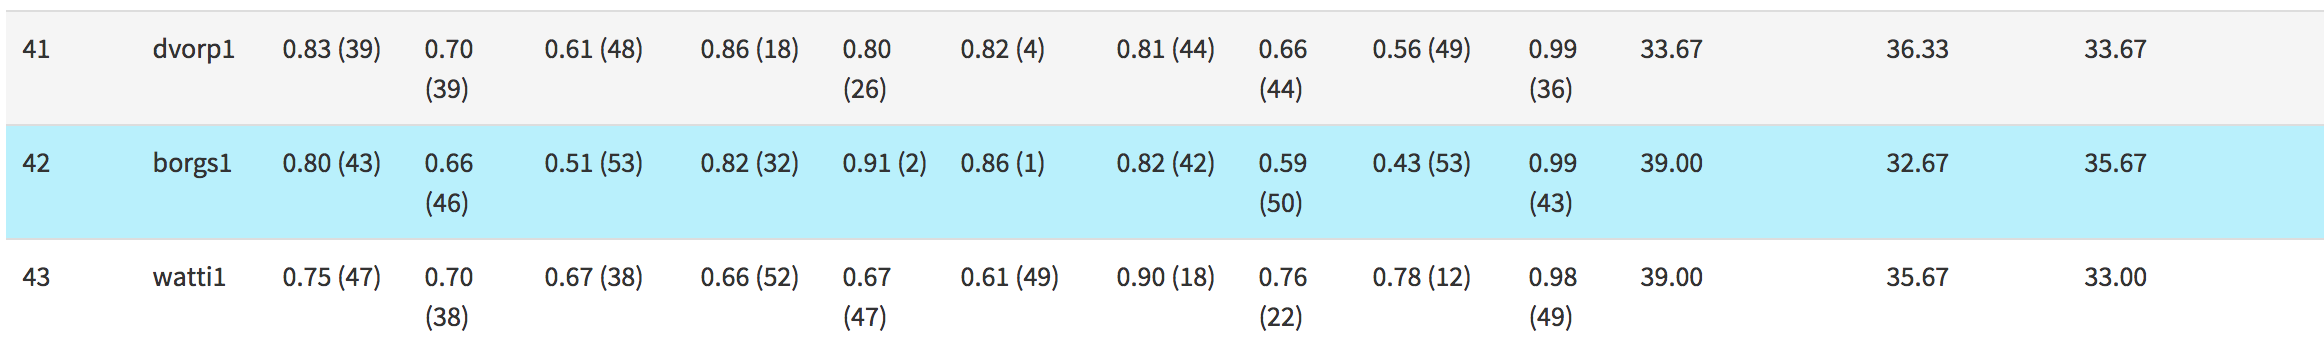
\includegraphics[width=\textwidth]{pereira_model_ranked_results}
	\caption{Online evaluation ranking. My submission was ranked 42\textsuperscript{nd}.}
\end{figure}

%\subsection{Effect of training duration}
%Pereira et al. trained this model for 20 epochs on about 450,000 patches per epoch. In figure \ref{fig:pereira_validation_loss}, I plotted the validation loss and the validation accuracy obtained on 500 patches for each class. Since the validation data is balanced, it does make sense to examine the accuracy as well as the other metrics. However, an increase in validation accuracy does not necessarily mean that the Dice score will improves as well. To investigate how the Dice score changes as the model is  trained, I saved the model after each epoch, meaning that I can segment the challenge scans after each epoch to investigate how the dice score changes. I plot the results in Figure \ref{fig:dice_training}. SAY SOMETHING ABOUT WHAT IS TO SEE IN THAT PLOT. TODO
%
%\begin{figure}
%	\centering
%	\label{fig:dice_training}
%	\setlength\figureheight{10cm}
%	\setlength\figurewidth{0.8\textwidth}
%	% This file was created by matplotlib2tikz v0.6.6.
\begin{tikzpicture}

\begin{axis}[
xlabel={Epoch},
ylabel={Dice score},
xmin=0, xmax=20,
ymin=0, ymax=0.8,
axis on top,
width=\figurewidth,
height=\figureheight,
tick pos=both,
legend entries={{Complete region},{Core},{Enhancing}},
legend style={at={(0.03,0.97)}, anchor=north west},
legend cell align={left}
]
\addplot [blue]
table {%
1 0.6917
2 0.7285
3 0.7345
4 0.7441
5 0.7638
6 0.7661
7 0.7739
8 0.7869
9 0
10 0.7885
11 0
12 0
13 0
14 0
15 0.7922
16 0.7877
17 0.7932
18 0.7905
19 0.7935
20 0.7922
};
\addplot [green!50.0!black]
table {%
0 0.6776
1 0.6539
2 0.6179
3 0.5955
4 0.6021
5 0.6063
6 0.611
7 0.6155
8 0
9 0.6318
10 0
11 0
12 0
13 0
14 0.6235
15 0.5985
16 0.6274
17 0.6166
18 0.6266
19 0.6228
};
\addplot [red]
table {%
0 0.6113
1 0.5439
2 0.4915
3 0.488
4 0.4772
5 0.4877
6 0.4713
7 0.4829
8 0
9 0.5151
10 0
11 0
12 0
13 0
14 0.4784
15 0.4615
16 0.4877
17 0.491
18 0.498
19 0.4915
};
\end{axis}

\end{tikzpicture}
%	\caption{Plot of the mean dice scores for the three regions as the model is trained.}
%\end{figure}


\subsection{Confusion matrix}
To get more insights into how the model behaves, I decided to segment 11 scans from the 2015 dataset, normalised identically. The dice scores obtained for these 11 scans are 0.681, 0.643 and 0.673 for the `Complete', `Core' and `Enhancing' regions respectively. The ground truth for these scans is put together slightly differently as to the 2013 dataset, which explains why the dice scores is lower for the `Complete' region. However, the scans are still similar enough for these scores and the confusion matrix to be relevant. The confusion matrix is shown in table \ref{table:confusion_pereira}. As expected from the dice scores, the model is doing well for classes 0 and 4, predicting over 64\% of the voxels in class 4 correctly. For classes 1, 2 and 3 the model is doing rather poorly, reaching no more than 38\% of correctly classified voxels. The especially low result for class 3, with only about 11\% of correctly classified voxels can be explained by the fact that there is less training data available for this class. Furthermore, the boundaries between class 2, 3 and 4 are somewhat subjective, meaning that different interpretation of the tissues are possible.

\begin{table}
\centering	
\setlength{\tabcolsep}{10pt}
\begin{tabular}{c c S[table-format=2.3] S[table-format=2.3] S[table-format=2.3] S[table-format=2.3] S[table-format=2.3]} 
& & \multicolumn{5}{c}{\textbf{Predicted}} \\
\rule{0pt}{3ex}& & \multicolumn{1}{c}{0} & \multicolumn{1}{c}{1} & \multicolumn{1}{c}{2} & \multicolumn{1}{c}{3} & \multicolumn{1}{c}{4} \\
\cline{3-7}
\multirow{5}{*}{\rotatebox[origin=c]{90}{\textbf{Ground truth}}} & \multicolumn{1}{c|}{0} & 99.94 & 0.001 & 0.052& 0.002 & 0.001 \\
& \multicolumn{1}{c|}{1} & 42.287 & 25.361 & 5.059 & 17.710 & 9.582 \\
& \multicolumn{1}{c|}{2} & 55.743 & 1.508 & 38.762 & 3.065 & 0.921 \\
& \multicolumn{1}{c|}{3} & 51.163 & 8.576 & 23.191 & 10.702 & 6.367 \\
& \multicolumn{1}{c|}{4} & 25.067 & 0.891 & 3.926 & 6.107 & 64.0078 \\
\end{tabular}
\caption{Confusion matrix for the model proposed by Pereira for 11 scans taken from the BraTS 2015 dataset. The percentage of correctly predicted voxels for each class is shown.}
\label{table:confusion_pereira}
\end{table}

\subsection{Effect of various components}
Finally, I investigate what impact different components and design choices for the convolutional neural networks have on the final dice score on the challenge dataset. I investigate the following desing choices:
\begin{enumerate}
	\item Using the linear rectifier (ReLU) activation function \ref{eq:linear_rectifier} instead of the Leaky linear rectifier.
	\item Using the Adaptive Moment Estimation method (adam) \cite{adam} to update the learning rates automatically, instead of linearly decaying the learning rate.
	\item Not performing any rotations during the data augmentation step.
	\item Only performing the N4 correction \cite{n4itk} and the mean and standard deviation normalisation during the pre-processing, i.e.\ leaving winsorising out.
\end{enumerate}
In table \ref{table:variants_dice_results} the results obtained using these variants are shown. The variant using the adam optimisation performs better than the proposed model which uses linearly decaying learning rates. This suggests that the model proposed might not have fully converged after 20 epochs and would need further training and learning rate adaptation to reach the same convergence as the model using the adam optimisation.

\begin{table}
\centering	
\begin{tabular}{ c | c c c} 
\multirow{2}{*}{\textbf{Variant}} & \multicolumn{3}{c}{\textbf{Dice score}} \\
 & Complete & Core & Enhancing \\
 \hline
Adam + ReLU & $0.796 \pm 0.054$ & $0.630 \pm 0.279$ & $0.486 \pm 0.265$ \\
Adam optimiser & $0.815 \pm 0.069$ & $0.670 \pm 0.233$ & $0.592 \pm 0.217$ \\
No rotations & Gather data points \\
No Winsorizing & Gather data points \\
\end{tabular}
\caption{Dice scores obtained using variants of the model proposed by Pereira et al.}
\label{table:variants_dice_results}
\end{table}


\section{Evaluation of my model}
\subsection{BraTS evaluation}
Table \ref{table:my_model_dice_results} shows the results I obtained using my fully-convolutional model on the 10 images included in the challenge dataset. The results for patient number 7 are again considerably lower than those obtained on the other patients in the `Core' and `Enhancing' regions. This is hard to explain, as Pereira reported no such discrepancy. A possible explanation, is that the images for patient 7 are slightly rotated in the x-y plane, as shown in figure \ref{fig:patient_7_t2}. In table \ref{table:class_frequencies}

\begin{table}
\centering	
\begin{tabular}{ c | c c c} 
\multirow{2}{*}{\textbf{Patient}} & \multicolumn{3}{c}{\textbf{Dice score}} \\
 & Complete & Core & Enhancing \\
 \hline
1 & 0.856 & 0.796 & 0.665 \\
2 & 0.843 & 0.622 & 0.670 \\
3 & 0.744 & 0.297 & 0.368 \\
4 & 0.379 & 0.156 & 0.150 \\
5 & 0.812 & 0.689 & 0.665 \\
6 & 0.772 & 0.381 & 0.493 \\
7 & 0.593 & 0.015 & 0.015 \\
8 & 0.877 & 0.705 & 0.675 \\
9 & 0.725 & 0.857 & 0.781 \\
10 & 0.898 & 0.905 & 0.838 \\
\textbf{mean} & $0.750 \pm 0.158$ & $0.542 \pm 0.310$ & $0.532 \pm 0.273$
\end{tabular}
\caption{Dice scores obtained for the 10 challenge patients using my model.}
\label{table:my_model_dice_results}
\end{table}

\begin{table}
\centering	
\begin{tabular}{ c | c | c} 
\textbf{Region} & \textbf{Mean sensitivity } & \textbf{Mean positive predictive value} \\
\hline
Complete &	$0.661 \pm 0.209$ & $0.933 \pm 0.042$ \\
Core & 		$0.453 \pm 0.318$ & $0.945 \pm 0.038$ \\
Enhancing & $0.467 \pm 0.297$ & $0.840 \pm 0.101$ \\
\end{tabular}
\caption{Sensitivity and positive predictive value for the three regions obtained on challenge dataset using my model.}
\label{table:my_model_sensitivity_ppv}
\end{table}

\begin{figure}[h]
	\centering
	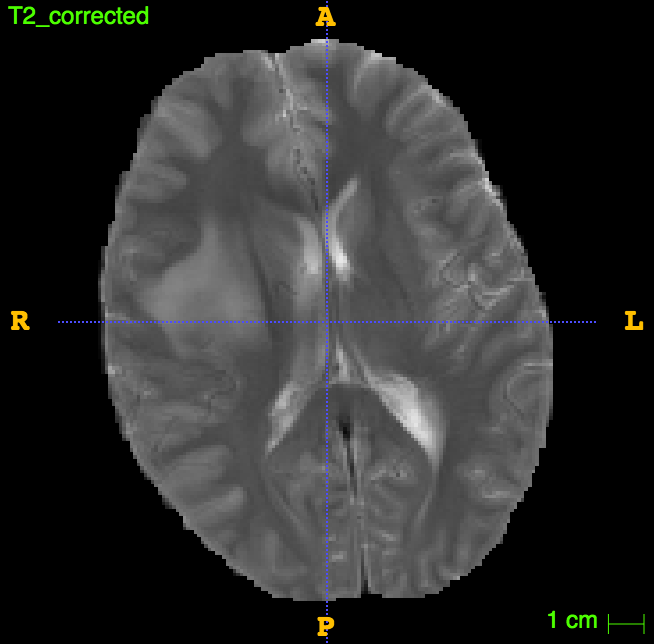
\includegraphics[scale = 0.3]{patient7_t2}
	\label{fig:patient_7_t2}
	\caption{Slice taken from the T2 scan for patient 7 of the challenge dataset. The image is slightly rotated in the x-y plane, which is a possible explanation for the lower results in the `Core' and `Enhancing' regions for that patient.}
\end{figure}

\subsection{Confusion matrix}
The confusion matrix obtained for my model using 11 of the BraTS2015 patients is shown in table \ref{table:confusion_my_model}. Interstingly, although my model performs worse on the 2013 challenge dataset than the model proposed by pereira et al., it performs much better on this subset of the 2015 training dataset, obtaining average dice scores of (0.806,0.776,0.819).

\begin{table}
\centering	
\setlength{\tabcolsep}{10pt}
\begin{tabular}{c c S[table-format=2.2] S[table-format=2.2] S[table-format=2.2] S[table-format=2.2] S[table-format=2.2]} 
& & \multicolumn{5}{c}{\textbf{Predicted}} \\
\rule{0pt}{3ex}& & \multicolumn{1}{c}{0} & \multicolumn{1}{c}{1} & \multicolumn{1}{c}{2} & \multicolumn{1}{c}{3} & \multicolumn{1}{c}{4} \\
\cline{3-7}
\multirow{5}{*}{\rotatebox[origin=c]{90}{\textbf{Ground truth}}} & \multicolumn{1}{c|}{0} & 99.78 & 0.02 & 0.16 & 0.02 & 0.02 \\
& \multicolumn{1}{c|}{1} & 0.74 & 42.66 & 20.58 & 26.91 & 9.11 \\
& \multicolumn{1}{c|}{2} & 28.79 & 4.13 & 57.97 & 7.54 & 1.57 \\
& \multicolumn{1}{c|}{3} & 5.87 & 10.49 & 30.81 & 37.98 & 14.84 \\
& \multicolumn{1}{c|}{4} & 4.44 & 1.62 & 4.77 & 8.52 & 80.64 \\
\end{tabular}
\caption{Confusion matrix obtained with my model for 11 scans taken from the BraTS 2015 dataset. The percentage of correctly predicted voxels for each class is shown.}
\label{table:confusion_my_model}
\end{table}

\chapter{Conclusion}
\section{Summary of achievements}
This project surveyed the mathematical foundations of deep learning with convolutional neural networks and how these models can be applied to the problem of brain tumour segmentation. I implemented two different convolutional neural networks. First, I replicated the model proposed by Pereira et al.\ \cite{pereira}. This gave me an introduction to this field with some certainty that the model would work. I then designed a second model using techniques more recently developed for the design of convolutional neural networks. The model I propose is performing similarly, but has the significantly advantage of being able to segment a scan much faster. This speed-up is achieved by removing all fully-connected layers from the network. This also has the effect of  reducing the number of parameters, meaning that my convolutional neural networks was able to consider an input patch with 4 times more voxels while keeping the number of parameters similar. Both models were trained on the data made available through the BraTS2013 challenge.

I evaluated both models using the standard metrics for this segmentation task: Dice score, positive predictive value and sensitivity. I also compared the performance of my models to the performance of models published by researchers in the field using the BraTS challenge leaderboard. Using the data from the BraTS 2015 dataset, I was further able to get more insight in how well the different models perform by examining the confusion matrix for this dataset.

Both models performed approximated the performance obtained by recent state-of-the-art methods for the `Complete' region, but not for the `Core' or `Enhancing' region. Especially noticeable is the difference in the Dice score for the `Enhancing' tumour region between my implementation of the model proposed  by Pereira et al. and their published results. After emailing the author, I was able to confirm that the only difference in implementation was the heuristic for selecting which patches to train the network on, which was not specified in the published paper. Hence, if I had to do it again, I would probably choose to replicate a more detailed paper or a paper for which the source code is available. This difference in results also shows the importance of the quality of the input data for deep learning methods, which often is more important than the architectural details of the network. Interestingly, increasing the receptive field of the neural network to a larger patch surrounding the voxels to classify did not significantly increase the performance of the network, meaning that the class of a voxel is highly dependent on the surrounding voxels but not on those voxels slightly further apart.

\section{Future Work}
A likely future direction is to use three-dimensional patches, instead of being restricted to two-dimensional patches. Incorporating the third dimension is challenging in convolutional neural networks due to the exponential growth in parameters associated with it. However, some very recent approaches have overcome these difficulties and use three-dimensional patches to achieve state-of-the-art results \cite{kamnitsas}. 

A further likely future direction concerns the fact that convolutional neural networks are not able to give any measure of uncertainty for their predictions, which might be very important for life-or-death cases such as brain tumours. Some recent work by Gal and Ghahramani showed how it is possible to get such uncertainty bounds in convolutional neural networks using Dropout \cite{Gal2015Dropout}. It would be interesting to research how this new knowledge could be incorporated into models for brain tumour segmentation.


%%%%%%%%%%%%%%%%%%%%%%%%%%%%%%%%%%%%%%%%%%%%%%%%%%%%%%%%%%%%%%%%%%%%%
% the bibliography
\addcontentsline{toc}{chapter}{Bibliography}
\bibliography{refs}

%%%%%%%%%%%%%%%%%%%%%%%%%%%%%%%%%%%%%%%%%%%%%%%%%%%%%%%%%%%%%%%%%%%%%
%% the appendices
\appendix

%\chapter{Latex source}
%
%\section{diss.tex}
%{\scriptsize\verbatiminput{diss.tex}}
%
%\section{proposal.tex}
%{\scriptsize\verbatiminput{proposal.tex}}


\chapter{Project Proposal}

% Note: this file can be compiled on its own, but is also included by
% diss.tex (using the docmute.sty package to ignore the preamble)
\documentclass[12pt,a4paper,twoside]{article}
\usepackage[pdfborder={0 0 0}]{hyperref}
\usepackage[margin=25mm]{geometry}
\usepackage{graphicx}
\usepackage{parskip}
\begin{document}

\begin{center}
\Large
Computer Science Tripos -- Part II -- Project Proposal\\[4mm]
\LARGE
Brain tumour segmentation using Convolutional Neural Networks

\large
S.~Borgeaud~dit~Avocat, Fitzwilliam College

Originator: D.~Wang

11 October 2016
\end{center}

\vspace{5mm}

\textbf{Project Supervisor:} Dr M.~Jamnik \& D.~Wang

\textbf{Director of Studies:} Dr R.~K.~Harle

\textbf{Project Overseers:} Prof J.~Bacon  \& Prof R.~Anderson

% Main document

\section*{Introduction}

Over the last years deep learning, more specifically convolutional neural networks (CNN), have outperformed other machine learning techniques in many tasks such as image classification \cite{nature-deep-learning-review}. The field of bioinformatics is no exception to this, in particular, convolutional neural networks have been shown to perform as well as previous state-of-the-art algorithms on the problem of brain tumour segmentation \cite{brats-proceedings}.

The aim of this project is to use convolutional neural networks to replicate these recent results on the brain tumour segmentation problem. This project will concentrate exclusively on the dataset provided by the BraTS2013\footnote{\url{http://martinos.org/qtim/miccai2013/}} grand challenge on which many different algorithms have already been tested and will provide a good framework to test and compare my work.

As a starting point I will follow the paper written by Pereira et al \cite{pereira}. The approach used is to cut the magnetic resonance images into multiple patches and regard the problem as a classification problem of the pixel located at the center of the patch. The aim is to classify each pixel into one of these four classes:
\begin{enumerate}
	\item Non-tumor
	\item Surrounding edema
	\item Non-enhancing tumour
	\item Enhancing tumour
\end{enumerate}
\section*{Starting point}
  
The starting point for this project is the part 1B course 'Artificial Intelligence 1'  which provided a short introduction to machine learning. In particular multi-layer perceptrons, the sigmoid activation function, backpropagation and stochastic gradient descent training were introduced. These concepts are all reused in convolutional neural networks which add convolutional and pooling layers to conventional multi-layer perceptrons network.

I will be using the Keras library with Tensor Flow to create and train convolutional neural networks.

Keras is a library written for Python. Fortunately, I have used Python before in small side projects meaning that I won't have to spend time learning a new language.

As the problem is self contained and formulated purely as a a machine learning task, none or very little biological/medical background knowledge is required.

\section*{Resources required}

For this project I will mainly use my own quad-core computer which
runs Mac OS X El Capitan. I accept full responsibility for this machine and I have made contingency plans to protect myself against hardware and/or software failure. In case of failure, I will be able to terminate my project using the MCS machines.  Backups will be to my external hard disk. Once a week, I will also copy all files to my Google Drive to add an extra level of redundancy in case of hardware failure. All written code will be under version control using git and will be backed up on a private GitHub repository at least daily while working on it. 

I will also need a computer with an external GPU to train the neural network in a reasonable amount of time. For this, I will be using the Cambridge High Performance cluster. Alternatively, if this is not possible, I will use a GPU that would be provided by the AI group.

\section*{Work to be done}

The project breaks down into the following phases:

\begin{enumerate}

\item The first phase of the project will be mainly focused on research during which I will learn how convolutional networks  work and read up on how they have been used on the brain tumour segmentation problem in different papers. I plan to complete the Stanford CS321n\footnote{\url{http://cs231n.github.io/}} course on convolutional neural networks that I have already started. I will also need to learn how to use the Keras and TensorFlow libraries and review some of the more advanced Python features that I haven't used recently.

\item The second phase will mainly be devoted to preparing the images obtained from the BRATS dataset. The images will need to be cut into patches each of which will have to be normalised. I will need to perform bias field correction as magnetic resonance images can exhibit non-uniformities that are the result of magnetic field variations rather than anatomical differences \footnote{\url{http://brainsuite.org/processing/surfaceextraction/bfc/}}. I will then need to perform intensity normalisation across the different images. Finally, I will need to add the correct label to each patch using the segmentation provided with the original training images.

\item The next step will be to use the prepared and normalised patches to train a convolutional neural network using the Keras library. This will require hyperparameter tuning using cross-validation to avoid overfitting. I will then construct segmented images using my convolutional neural network to delimit the different segments to get a visual result that is easy to interpret.

\item During the last step I will evaluate how well my convolutional neural network performed using standard methods used to evaluate classifiers such as the confusion matrix, recall, precision and Dice scores. This evaluation can be done for different hyperparameters. Because the dataset has been used many times before as part of the Grand Challenge\footnote{\url{https://grand-challenge.org}} I will also be able to perform a quantitative comparison with different segmentation algorithms also using convolutional neural networks as well as other algorithms using different techniques.

\end{enumerate}

\section*{Success criteria}

The main success criteria for this project will be to have an algorithm that performs brain tumour segmentation into the 4 different segments as discussed earlier. 

The primary aim is to achieve similar results to those obtained by Pereira et al \cite{pereira}, hopefully achieving 90\% of the accuracies obtained in the paper. This means achieving the Dice\footnote{\url{https://en.wikipedia.org/wiki/Sorensen-Dice\_coefficient}} scores summarised in the following table, where `complete' refers to the complete tumour region (including classes 2--4), `core' refers to all regions except for the edema structure (classes 3--4) and `enhancing' includes only the enhancing tumour (class 4):

\begin{center}
\begin{tabular}{ |c|c|c| } 
\hline
complete & core & enhancing \\
\hline
 0.79 & 0.74 & 0.69  \\ 
\hline
\end{tabular}
\end{center}



\section*{Possible extensions}

Due to the recent development of this area, this project naturally leads to multiple possible extensions:
\begin{enumerate}
	\item This process of segmenting MRI scans is very slow as each scan has to be cut into patches, one per pixel, and each patch then needs to be classified. Recent techniques have shown that it is possible to classify all pixels of a patch at once, which would drastically improve the speed of the segmentation. A possible extension would be to try to improve the segmentation speed using the suggested technique. It would then be interesting to compare the performance of the faster algorithm to the performance of the original one.
	\item Experiment with the layout of the neural network, in particular change the number of layers and the type of the layers of the convolutional neural network to try to improve the accuracy.
	\item Instead of using the Keras library, implement similar functionality myself using TensorFlow. I could then compare the results obtained by my implemention with those obtained using Keras. This will show and require a deeper understanding of how convolutional neural networks work.
	\item Use different data prepocessing/normalisation techniques and analyse how they affect the final accuracy of the convolutional neural network.
	\item Apply more recent techniques used to improve convolutional neural networks such as Dropout \cite{dropout}, Maxout \cite{maxout} or Batch Normalization \cite{batch_normalization} in order to improve the accuracy of the classification.
\end{enumerate}

\section*{Timetable}

Planned starting date is 21/10/2016.

\subsection*{Michaelmas term}
\begin{enumerate}
\item \textbf{Weeks 3--4} Learn about Convolutional Neural Networks by finishing the CS321n online course. Read papers about using Convolutional Neural Networks for brain tumour segmentation.

\emph{Milestone:} Understand the theory behind convolutional neural networks and be familiar with some of the more recent applications of them on the brain tumour segmentation problem.

\item \textbf{Weeks 5--6} Become familiar with the Keras library and refresh my Python knowledge. Download and play with the dataset.

\emph{Milestone:} Be comfortable enough with Keras and Python to be able to start the main part of the project.

\item \textbf{Weeks 7--8} Prepare the dataset for the implementation of the convolutional neural network. This includes performing the different normalisations.

{Milestone:} Have the dataset ready, that is split up into normalised patches. Each patch should have the corresponding label for the pixel that is located at its center.

\item \textbf{Christmas Vacation} Implement and train a convolutional neural network and perform the necessary cross-validation on the different hyperparameters. Create segmented brain images using my classifier.

{Milestone:} Have a working convolutional neural network that is able to classify the different patches with the required accuracy mentioned in the primary success criteria. Have some images that are segmented using the trained classifier.
\end{enumerate}


\subsection*{Lent term}
\begin{enumerate}

\item \textbf{Weeks 1--3} Write the progress report and prepare the presentation.

{Milestone:} Have the progress report submitted on time and be ready to give the presentation.

\item \textbf{Weeks 4--5} Evaluate the performance of my segmentation algorithm and look for possible improvements.

{Milestone:} Have the evaluation data of my convolutional neural network.

\item \textbf{Weeks 6--8} Compare the performance of my algorithm with the benchmarks available online and implement some of the extensions if time permits.

{Milestone:} Have all the necessary data for the final evaluation of my project.

\item \textbf{Easter Vacation} Write the main chapters of the dissertation. Implement some of the extensions if time permits.

{Milestone:} Have a complete first draft of my dissertation

\end{enumerate}

\subsection*{Easter term}
\begin{enumerate}
\item \textbf{Weeks 1--2} Improve the dissertation where necessary

{Milestone:} Have the dissertation in its final form
\item \textbf{Weeks 3--4} Proof read the dissertation and submit it.

{Milestone:} Have the dissertation submitted.

\end{enumerate}

\end{document}

\end{document}
